\documentclass{thesis}

%%%%%%%%%% LANGUAGE SELECTION %%%%%%%%%%

% Use German. Swap the % before the following two lines for an english thesis:
%\Germantrue
\Germanfalse

%%%%%%%%%% PACKAGES %%%%%%%%%%
% Put additional packages here
\usepackage[normalem]{ulem}
\useunder{\uline}{\ul}{}
\usepackage{booktabs}
\usepackage{float}
\usepackage{multirow}
\usepackage{amsmath}
\usepackage{amssymb}
\usepackage{hyperref}
\usepackage{verbatim}
\usepackage{scrhack}
\usepackage{needspace}
\usepackage{ragged2e}
\usepackage{placeins}
\usepackage{stfloats}
\usepackage{subcaption}
\usepackage[ruled,vlined]{algorithm2e}


%%%%%%%%%% CONFIGURATION %%%%%%%%%%
\thesistype{\Master} % Or \Master or a custom string
\title{Transformers are all you need? Forecasting human motion with attention!}
\author{Denis Gosalci}
\authorgender{m} % or "f"
\birthdate{10.05.1999}
\birthloc{Nuremberg}
\thesisstart{01.04.2024}
\thesisend{30.09.2024}
\institute{\FAUIPSG}
\instituteloc{Erlangen}
\thesissupervisor{Tobias Feigl} % Can be used multiple times

% Fill in the following according to the entry in UnivIS for the thesis
\begin{thesisbackground}
Forecasting methods for the stock market, electricity prices, or weather and climate are ubiquitous and are extensively researched [1]. However, forecasting human motion in sports is only sparsely researched. Here too, forecasting technology is crucial to compress system delays at an early stage, reduce injuries, achieve tactical advantages [2] and, in short, improve analysis before, during, and post-game [3]. For instance, coaches draw more effective decisions, such as switching players for health reasons due to irregular motion. The demand for forecasting methods is currently increasing with newly emerging communication platforms, e.g., 6G, and the Internet of Things. However, forecasting human motion, especially their positions, is a difficult task as human motion is practically indeterministic. Scenarios with fast and unpredictable human motion, e.g., in sports such as NBA basketball, render forecasting virtually impossible. So, experts explore forecasting models that can accurately, reliably, promptly, and as far as possible forecast people’s future motion in complex and dynamic environments. For this purpose, classic Bayesian methods such as Kalman and particle filters (KF, PF) [4] were developed. However, these linear models do not remember the motion history necessary to forecast more than just a single time step of the future. In sport, KF and PF are practically ineffective when people move with rapid changes in speed and acceleration and influence each other (tactically) during the course of the game. That is why promising AI approaches have recently been explored. These methods have the potential to exploit nonlinear patterns in dynamic, complex motion that even experts miss as their nonlinear learning capabilities handle the “stochastic” nature of sports motion. The idea is that artificial intelligence (AI) observes, interprets, and learns the movement patterns, their connections and influences, remembers the history and evolution of patterns so that, equipped with this knowledge, the AI is able to forecast complex and dynamic (indeterministic) motion. Recently, Vaswani et al. [5] introduced the most prominent Transformer model that leverages the self-attention mechanism to increase the number of memorable time steps, thus surpassing traditional recurrent neural networks (RNNs) such as LSTMs [6] and LMU [7] w.r.t. accuracy and robustness. Transformers offer the advantages of convolutional networks (optimal feature extraction) and RNNs (memory) and are robust against very large input data spaces with very high information complexity and dimensionality. A well-known example of a Transformer-based model is Chat-GPT for natural language data processing [8] or TimeGPT for time series data processing [1]. However, there is currently no Transformer model for (multivariate and multi-task) forecasting of motion in sport.\\
\end{thesisbackground} 
\begin{thesistask}
The literature leaves it unclear why more memory of LMU and attention cells does not necessarily result in higher accuracy and robustness than LSTM cells. Therefore, the student will examine the performance of LSTM and LMU cells and Transformer (attention) architecture on NBA data and evaluate the impact of time scale, memory, and parameters on accuracy, robustness, uncertainty, and forecast horizon. Since previous work trained individual Transformer models for each pedestrian to estimate person-specific positions, the information-rich (social) context between pedestrians is lost. It is unclear how (social) interactions and contexts can be represented in Transformer models. It is also unclear how and whether Transformers lead to more accurate, robust, and comprehensive forecasts than the state-of-the-art. The student will thus explore various LSTM, LMU, classic Transformer, BitNet, and (optionally) RetNet models for multivariate and multi-task forecasting of motion in sports. The student investigates the effects of input dimensions (a single player up to a maximum of 10 NBA players per game) on the accuracy, robustness, uncertainty, and forecast horizon of Transformer-like models. Since it is also unclear how and whether precompiled Transformers such as TimeGPT can be adapted on multivariate and multi-tasking human movement forecasting in sports applications. The student will investigate whether and how we can define and generate input embeddings with at least two players so that TimeGPT may forecast at least the positions of a single player. The student will also examine the effects of splitting the position into univariate input embeddings, i.e., x- and y-coordinates, to forecast only x- and y-coordinates. He will compare different embeddings and optimizations of LSTM, LMU, a classic Transformer, TimeGPT, BitNet, and (optionally) RetNet and reports performance and computational complexity. The student will also examine how these models can be adapted or fine-tuned to sports motion. The student will conduct an ablation study that optimizes and evaluates all (possible) methods in terms of: velocity versus position input information; length of historical context versus forecast horizon; impact on the forecast horizon; training and inference time. For all benchmarks, the student employs at least the following metrics: Mean Absolute Error (MAE), Root Mean Square Error (RMSE), Average Displacement Error (ADE), and Final Displacement Error (FDE)[14]. A graphical evaluation compares the positioning results.
\end{thesistask}

\thesismilestone{3 PW Literature review.}
\thesismilestone{3 PW Preprocessing of data sets, e.g., NBA [15].}
\thesismilestone{4 PW Implementation of a (parameterizable) software framework for forecasting human motion.}
\thesismilestone{6 PW Adaptation and implementation of methods such as LSTM [6], LMU [7], Transformer [5], TimeGPT [1], BitNet [9], and (optionally) RetNet [10].}
\thesismilestone{4 PW Optimization and evaluation of the methods along an ablation study, e.g., effects of input (contextual) dimension, computational complexity, forecast horizon, storage capacity, and metrics such as Mean Absolute Error (MAE), Root Mean Square Error (RMSE), Average Displacement Error (ADE), Final Displacement Error (FDE) and Average Non-linear displacement error (NL-ADE) [14].}
\thesismilestone{4 PW Transcript.}


\thesisliterature{[1] A. Garza and M. Mergenthaler-Canseco, ``TimeGPT-1'' arXiv: 2310.03589 [cs.LG], pp. 1-–12, 2023. doi: 10.48550/arXiv.2310.03589.}
\thesisliterature{[2] L. Lamas, J. Barrera, G. Otranto, and C. Ugrinowitsch, ``Invasion Team Sports: Strategy and Match Modeling'' Intl. Jo. of Performance Analysis in Sport, vol. 14, no. 1, pp. 307–-329, 2014. doi: 10.1080/24748668.2014.11868723.}
\thesisliterature{[3] J. Gudmundsson and M. Horton, ``Spatio-Temporal Analysis of Team Sports'' ACM Computing Surveys (CSUR), vol. 50, no. 2, pp. 1–-42, 2017. \\ doi: 10.48550/arXiv.1602.06994.}
\thesisliterature{[4] T. Feigl, ``Datengetriebene Methoden zur Bestimmung von Position und Orientierung in funk- und trägheitsbasierter Koppelnavigation'' Dr.-Ing. Dissertation, Technische Fakultät der Friedrich-Alexander-Universität Erlangen-Nürnberg, 2021.}
\thesisliterature{[5] A. Vaswani, N. Shazeer, N. Parmar, J. Uszkoreit, L. Jones, A. N. Gomez, L. Kaiser, and I. Polosukhin, ``Attention Is All You Need'' arXiv:1706.03762 [cs.CL], pp. 1–-15, 2017. doi: 10.48550/arXiv.1706.03762.}
\thesisliterature{[6] S. Hochreiter and J. Schmidhuber, ``Long short-term memory'' Neural computation, vol. 9, no. 8, pp. 1735–-1780, 1997. doi: 10.1162/neco.1997.9.8.1735.}
\thesisliterature{[7] A. Voelker, I. Kaji\'{c} and C. Eliasmith, ``Legendre Memory Units: Continuous-Time Representation in Recurrent Neural Networks'' in Proc. of Conf. Advances in Neural Information Processing Systems (NIPS), Vancouver, Canada, 2019, pp. 15544-–15553. [Online]. Available: https://papers.nips.cc/paper\_files/paper/2019/file/\\952285b9b7e7a1be5aa7849f32ffff05-Paper.pdf.}
\thesisliterature{[8] OpenAI, ``GPT-4 Technical Report'' arXiv:2303.08774v3 [cs.CL], pp. 1–-100, 2023. doi: 10.48550/arXiv.2303.08774.}
\thesisliterature{[9] H. Wang, S. Ma, L. Dong, S. Huang, H. Wang, L. Ma, F. Yang, R. Wang, Y. Wu, and F. Wei, ``BitNet: Scaling 1-bit Transformers for Large Language Models'' arXiv: 2310.11453 [cs.CL], pp. 1–-14, 2023. doi: 10.48550/arXiv.2310.11453.}
\thesisliterature{[10] Y. Sun, L. Dong, S. Huang, S. Ma, Y. Xia, J. Xue, J. Wang, and F. Wei, ``Retentive Network: A Successor to Transformer for Large Language Models'' arXiv: 2307.08621 [cs.CL], pp. 1–-14, 2023. doi: 10.48550/arXiv.2307.08621.}
\thesisliterature{[11] S. Hauri, N. Djuric, V. Radosavljevic, and S. Vucetic, ``Multi-Modal Trajectory Prediction of NBA Players'' in Proc. of IEEE Winter Conf. on Applications of Computer Vision (WACV), Waikoloa, HI, 2021, pp. 1639–-1648. \\ doi: 10.1109/WACV48630.2021.00168.}
\thesisliterature{[12] D. Gosalci, ``Legendre Memory Unit'' Bachelor’s Thesis, Technische Hochschule Georg-Simon-Ohm Nürnberg, 2021.}
\thesisliterature{[13] F. Giuliari, I. Hasan, M. Cristani, and F. Galasso, ``Transformer Networks for Trajectory Forecasting'' arXiv:2003.08111 [cs.CV], pp. 1–-14, 2020. doi: 10.48550/arXiv.2003.08111.}
\thesisliterature{[14] K. Xu, Z. Qin, G. Wang, K. Huang, S. Ye, and H. Zhang, ``Collision-Free LSTM for Human Trajectory Prediction'' in Proc. of MultiMedia Modeling, Bangkok, Thailand, 2018, pp. 106–-116. doi: 10.1007/978-3-319-73603-7\_9.}
\thesisliterature{[15] K. Linou, D. Linou, and M. de Boer, ``NBA Player Movements Dataset'' 2016. [Online]. Available: https://github.com/linouk23/NBA-Player-Movements.}



%%%%%%%%%% BIBLIOGRAPHY %%%%%%%%%%

% Put all references in the file references.bib in BibTeX format. Please pay
% attention to some common errors when writing references:
% https://www.ece.ucdavis.edu/~jowens/biberrors.html
\addbibresource{references.bib}



%%%%%%%%%% DOCUMENT %%%%%%%%%%
\begin{document}


%%%%%%%%%% COVER %%%%%%%%%%
% Cover muss separat kompiliert werden über "cover.tex" mit xetex / luatex compiler
% Das pdf muss herunter- und hier wieder hochgeladen werden!
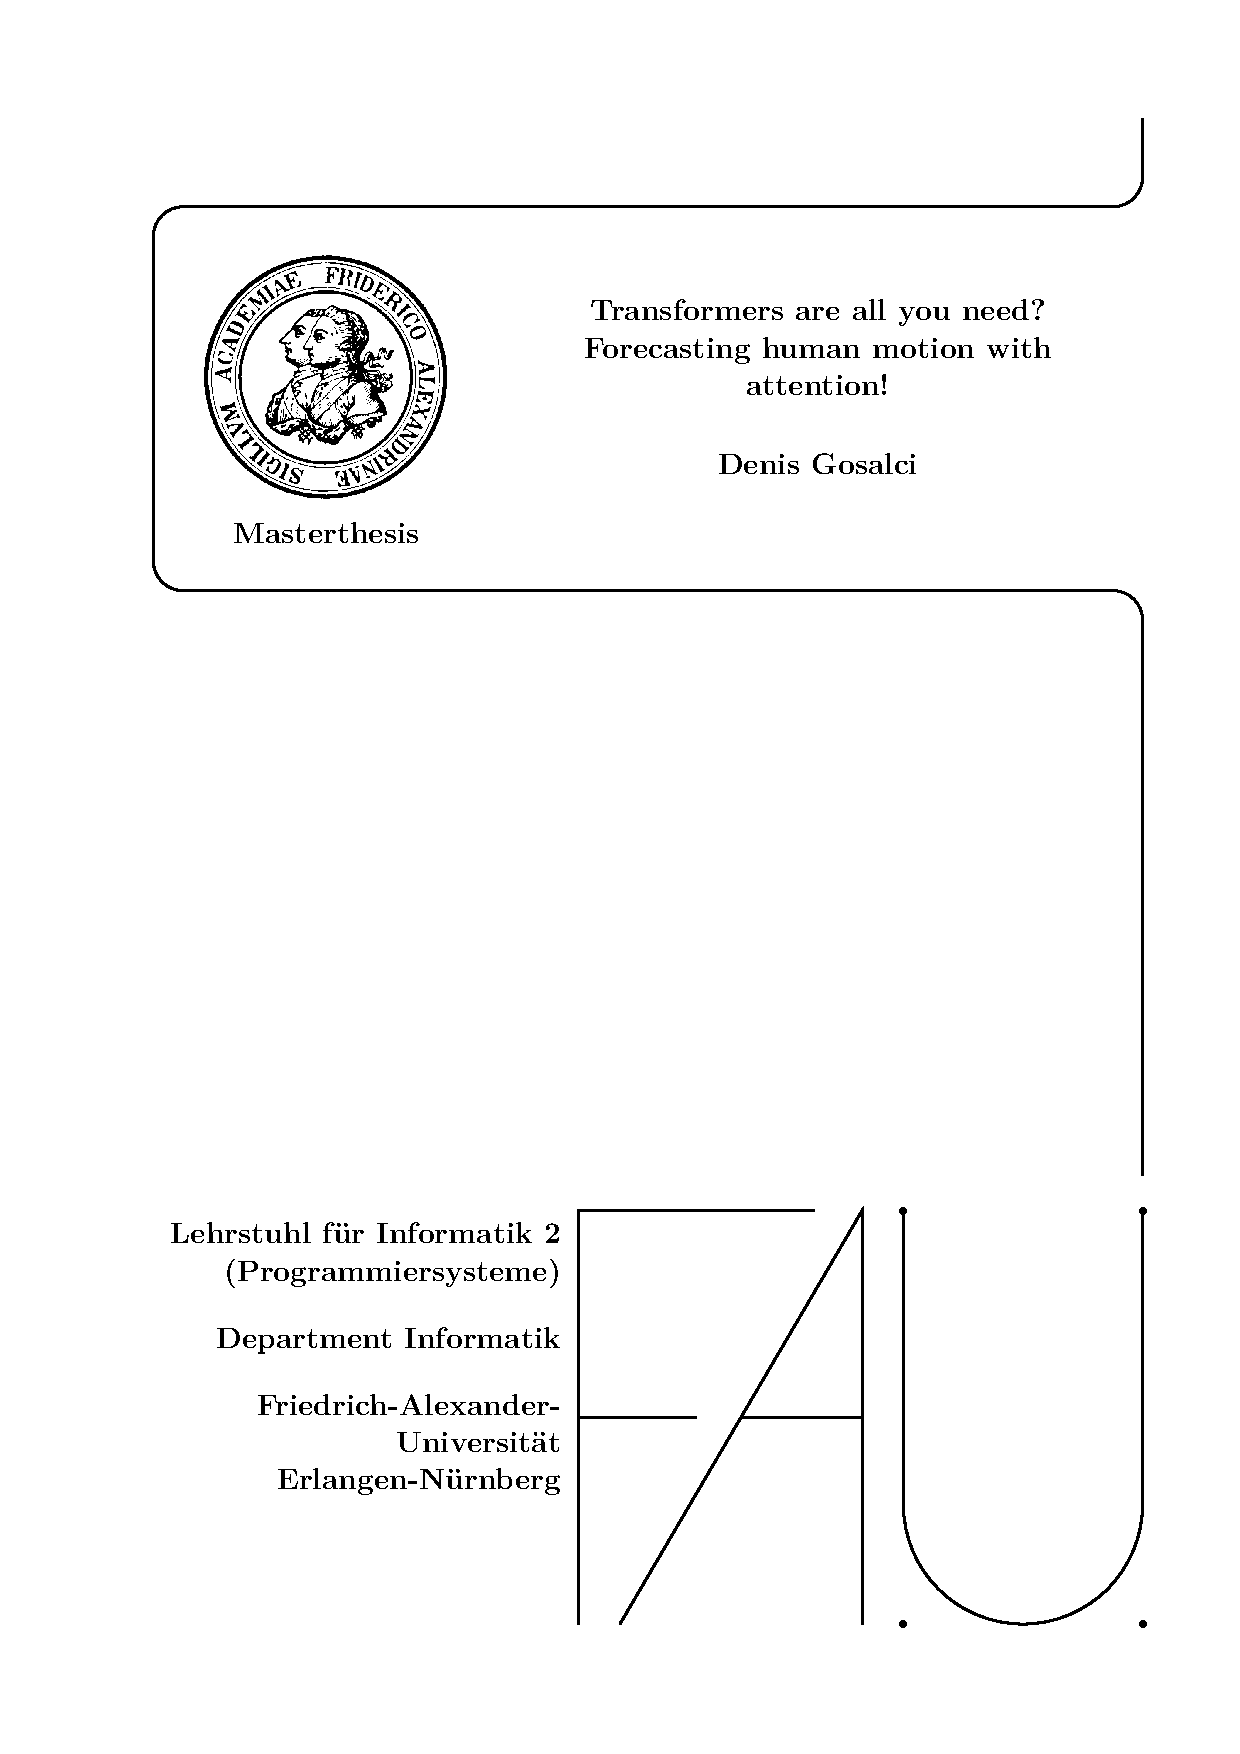
\includepdf[pages=-]{cover.pdf}

\MakeTitlePage

\MakePledgePage % Or (only in rare cases!) \MakePledgePage[nogrant]

\MakeTaskPage

\begin{abstract}{german}
Die Vorhersage menschlicher Bewegungen spielt eine entscheidende Rolle in Bereichen wie der Sportanalyse (SA), der Verletzungsprävention und der Optimierung von Spielstrategien. Die genaue Vorhersage von Bewegungen in dynamischen, Echtzeitumgebungen, wie beispielsweise bei Basketballspielen, stellt jedoch eine erhebliche Herausforderung dar, da menschliche Bewegungen oft unvorhersehbar und stark variabel sind. Traditionelle Vorhersagemodelle, wie Kalmanfilter (KF) und Partikelfilter (PF), erweisen sich in solchen Kontexten häufig als ineffektiv, da sie die nichtlinearen und stochastischen Eigenschaften schneller Sportarten nicht erfassen können. Neuere Fortschritte rekurrenten neuronalen Netzen (RNNs) wie Long Short-Term Memory (LSTM) und Legendre Memory Units (LMUs), haben vielversprechende Ansätze gezeigt, diese Einschränkungen zu überwinden. Dennoch haben auch diese Modelle Probleme mit der Speicherung langer Zeitfolgen und der Verarbeitung gro{\ss}er~Datensätze.

Wir untersuchen in dieser Arbeit das Potenzial von Transformer-basierten Modellen, die durch ihren Self-Attention-Mechanismus (SAM) bekannt sind, um die Genauigkeit und Robustheit der Vorhersage menschlicher Bewegungen zu verbessern. SAM ermöglicht es Transformern, gro{\ss}e zeitliche Abhängigkeiten und Nichtlinearitäten in den Daten zu erfassen, was sie besonders geeignet für komplexe, multivariate und Multi-Task-Bewegungsvorhersagen macht. Wir vergleichen die Leistung von LSTM-, LMU- und Transformer-Architekturen anhand von dynamischen Sportdatensätzen, mit besonderem Fokus auf die Bewegungen von NBA-Spielern. Insbesondere untersuchen wir, wie diese Modelle mit unterschiedlichen historischen Kontexten, Vorhersagehorizonten und Eingabedatenkonfigurationen – einschlie{\ss}lich positionsbasierter, geschwindigkeitsbasierter und kombinierter Eingaben – umgehen. Zusätzlich testen wir die Generalisierbarkeit der Modelle über verschiedene Teams hinweg, indem wir sie beispielsweise auf den Los Angeles Lakers (LAL) trainieren und die Generalisierung auf die Toronto Raptors (TOR)~prüfen. 

Unsere Ergebnisse zeigen, dass Transformer-Modelle die rekurrenten Architekturen hinsichtlich Genauigkeit, Robustheit und Vorhersagehorizont bei der Anwendung auf multivariate Sportdaten übertreffen. Allerdings gehen sie auch mit einer höheren Rechenkomplexität einher. Es zeigte sich zudem, dass die Kombination von Positions- und Geschwindigkeitsdaten zu genaueren Vorhersagen führt und multivariate Modelle gegenüber univariaten Ansätzen überlegen sind. Durch eine Reihe von Ablationsstudien identifizieren wir die optimalen Konfigurationen für die Vorhersage menschlicher Bewegungen in Sportanwendungen. Diese Arbeit liefert Einblicke, wie KI-Modelle, insbesondere Transformer, an Echtzeit-Umgebungen mit hohen Anforderungen angepasst werden können, und bildet die Grundlage für zukünftige Entwicklungen im Bereich der~SA.
\end{abstract}

\begin{abstract}{english}
Predicting human movements plays a crucial role in areas such as sports analysis (SA), injury prevention, and optimization of game strategies. However, accurately predicting movements in dynamic, real-time environments, such as basketball games, presents a significant challenge because human movements are often unpredictable and highly variable. Traditional prediction models, such as Kalman filters (KF) and particle filters (PF), often prove ineffective in these contexts as they fail to capture the nonlinear and stochastic characteristics of fast-paced sports. Recent advances in deep learning models, particularly recurrent neural networks (RNNs) such as Long Short-Term Memory (LSTM) and Legendre Memory Units (LMUs), have shown promising approaches to overcoming these limitations. Nevertheless, these models also face issues with storing long sequences and processing large datasets.

In this work, we explore the potential of Transformer-based models, known for their Self-Attention Mechanism (SAM), to improve the accuracy and robustness of human movement prediction. SAM enables Transformers to capture long-range temporal dependencies and nonlinearities in the data, making them particularly suited for complex, multivariate, and multi-task movement predictions. We compare the performance of LSTM, LMU, and Transformer architectures using dynamic sports datasets, with a particular focus on NBA player movements. Specifically, we investigate how these models handle different historical contexts, prediction horizons, and input data configurations—including position-based, speed-based, and combined inputs. Additionally, we test the generalizability of the models across different teams by training them, for example, on the Los Angeles Lakers (LAL) and evaluating generalization on the Toronto Raptors~(TOR).

Our results show that Transformer models outperform recurrent architectures in terms of accuracy, robustness, and prediction horizon when applied to multivariate sports data. However, they also come with higher computational complexity. We also found that combining position and speed data leads to more accurate predictions and that multivariate models are superior to univariate approaches. Through a series of ablation studies, we identify the optimal configurations for predicting human movements in sports applications. This work provides insights into how AI models, particularly Transformers, can be adapted to real-time environments with high demands and lays the groundwork for future developments in the field of SA.
\end{abstract}




\listoftodos

\tableofcontents
\listoffigures
\listofalgorithms
\listoftables

\newabbreviation{iot}{IoT}{Internet of Things}
\newabbreviation{sam}{SAM}{Self-Attention Mechanism}
\newabbreviation{svm}{SVM}{Support Vector Machine}
\newabbreviation{bloom}{BLOOM}{BigScience Large Open-science Open-access Multilingual Language Model}
\newabbreviation{bert}{BERT}{Bidirectional Encoder Representations from Transformers}
\newabbreviation{opt}{OPT}{Open Pre-trained Transformer}
\newabbreviation{llama}{LLaMA}{Large Language Model Meta AI}
\newabbreviation{nba}{NBA}{National Basketball Assoziation}
\newabbreviation{dfl}{DFL}{Deutsche Fu{\ss}ball Liga}
\newabbreviation{kf}{KF}{Kalman Filter}
\newabbreviation{pf}{PF}{Particle Filter}
\newabbreviation{ai}{AI}{Artificial Intelligence}
\newabbreviation{rnn}{RNN}{Recurrent Neural Network}
\newabbreviation{lstm}{LSTM}{Long Short-Term Memory}
\newabbreviation{lmu}{LMU}{Legendre Memory Unit}
\newabbreviation{retnet}{RetNet}{Retention Network}
\newabbreviation{mha}{MHA}{Multi-Head Attention}
\newabbreviation{sdpa}{SDPA}{Scaled Dot-Product Attention}
\newabbreviation{vgp}{VGP}{Vanishing Gradient Problem}
\newabbreviation{ts}{TS}{time series}
\newabbreviation{nlp}{NLP}{Natural Language Processing}
\newabbreviation{tanh}{tanh}{hyperbolic tangent}
\newabbreviation{relu}{ReLU}{Rectified Linear Unit}
\newabbreviation{lp}{LP}{Legendre Polynomial}
\newabbreviation{zoh}{ZOH}{zero-order hold}
\newabbreviation{sota}{SOTA}{State-of-the-Art}
\newabbreviation{llm}{LLM}{Large Language Model}
\newabbreviation{gelu}{GELU}{Gaussian Error Linear Unit}
\newabbreviation{ffn}{FFN}{Positionwise Feed-Forward Network}
\newabbreviation{tl}{TL}{Transfer Learning}
\newabbreviation{mse}{MSE}{Mean Squared Error}
\newabbreviation{nn}{NN}{Neural Network Model}
\newabbreviation{1ll}{1L Linear}{one layer Linear}
\newabbreviation{2ll}{2L Linear}{two layer Linear}
\newabbreviation{cpu}{CPU}{Central Processing Unit}
\newabbreviation{gpu}{GPU}{Graphical Processing Unit}
\newabbreviation{ide}{IDE}{Integrated Development Environment}
\newabbreviation{mae}{MAE}{Mean Absolute Error}
\newabbreviation{ade}{ADE}{Average Displacement Error}
\newabbreviation{fde}{FDE}{Final Displacement Error}
\newabbreviation{de}{DE}{Displacement Error}
\newabbreviation{aae}{AAE}{Anvergae Angular Error}
\newabbreviation{fae}{FAE}{Final Angular Error}
\newabbreviation{nlade}{NL-ADE}{Average Non-Linear Displacement Error}
\newabbreviation{ae}{AE}{Angular Error}
\newabbreviation{trafo}{Trafo}{Transformer}
\newabbreviation{m}{M}{Million}
\newabbreviation{mb}{MB}{Megabyte}


\glsxtrnewsymbol[description={Bias term for output \( x \)}]{bx}{\(b_x\)}
\glsxtrnewsymbol[description={Weight matrix mapping input \( x \) to output \( y \)}]{Wxy}{\(W_{xy}\)}
\glsxtrnewsymbol[description={Sigmoid activation function}]{sigmoid}{\(\sigma\)}
\glsxtrnewsymbol[description={Hidden state vector at time step \( t \)}]{h}{\(h_t\)}
\glsxtrnewsymbol[description={Hyperbolic tangent activation function}]{tanh2}{\(\tanh\)}
\glsxtrnewsymbol[description={Hadamard product (element-wise multiplication)}]{hadamard}{\(\odot\)}
\glsxtrnewsymbol[description={Input gate at time step \( t \)}]{it}{\(i_t\)}
\glsxtrnewsymbol[description={Forget gate at time step \( t \)}]{ft}{\(f_t\)}
\glsxtrnewsymbol[description={Cell state gate at time step \( t \)}]{gt}{\(g_t\)}
\glsxtrnewsymbol[description={Output gate at time step \( t \)}]{ot}{\(o_t\)}

\glsxtrnewsymbol[description={Window length parameter}]{theta}{\(\theta\)}
\glsxtrnewsymbol[description={Addition operator}]{addition}{$+$}

\glsxtrnewsymbol[description={Memory state at time step \( t \)}]{memory_state}{$m_t$}
\glsxtrnewsymbol[description={Processed input of the LMU at time step \( t \)}]{ut}{$u_t$}
\glsxtrnewsymbol[description={State space matrices}]{ab}{$A$, $B$}
\glsxtrnewsymbol[description={Discrete state space matrices}]{dab}{$\Bar{A}$, $\Bar{B}$}

\glsxtrnewsymbol[description={Activation function applied to vector \( x \)}]{f}{$f(x)$}
\glsxtrnewsymbol[description={Model dimensionality (hidden size)}]{d_model}{$d_{model}$}

\glsxtrnewsymbol[description={Query vector}]{q}{$Q$}
\glsxtrnewsymbol[description={Key vector}]{k}{$K$}
\glsxtrnewsymbol[description={Value vector}]{v}{$V$}

\glsxtrnewsymbol[description={Sum over all entries \( j \) in the vector}]{sum}{$\sum_j$}

\glsxtrnewsymbol[description={Mean of vector \( x \)}]{mean}{E[x]}
\glsxtrnewsymbol[description={Variance of vector \( x \)}]{var}{Var[x]}
\glsxtrnewsymbol[description={Machine epsilon for numerical stability}]{epsilon}{$\epsilon$}
\glsxtrnewsymbol[description={Learnable shift parameter}]{beta}{$\beta$}
\glsxtrnewsymbol[description={Learnable scale parameter}]{gamma}{$\gamma$}
\glsxtrnewsymbol[description={Sign function (returns the sign of the input)}]{sign}{sign(x)}
\glsxtrnewsymbol[description={Multiplication operator}]{times}{\times}
\glsxtrnewsymbol[description={Difference in time}]{delta_t}{$\Delta t$}

\glsxtrnewsymbol[description={2-norm of vector \( x \)}]{norm}{$\|x\|$}
\glsxtrnewsymbol[description={Final time step for prediction}]{t_p}{$T_{pred}$}
\glsxtrnewsymbol[description={Final time step for observation}]{t_o}{$T_{obs}$}

\printunsrtglossary[type=symbols, title={List of Symbols}]

\setlength{\parindent}{0pt} % damit die Zeilen immer bei ganz links anfangen

\mainmatter
\chapter{Introduction}
This Chapter provides a comprehensive overview of the research undertaken to enhance the forecasting of human motion in team-based sports. It begins by addressing the motivation behind this study and outlines the specific problem statement that drives the inquiry (see Section \ref{sec:motivation}). Following this, the Chapter articulates the research questions that guide the investigation (see Section \ref{sec:research_questions}), highlighting the key areas of focus that emerge from the problem statement.

Subsequently, the proposed solutions to these questions are discussed, detailing the methodologies and models applied in this research (see Section \ref{sec:solution}). This is followed by an examination of the findings derived from the analysis, offering insights into the effectiveness of the various approaches explored (see Section \ref{sec:findings}). Finally, the Chapter concludes with an outline of the subsequent Sections, summarizing how the research contributes to the broader field of human motion forecasting and the implications of the findings for future work (see Section \ref{sec:outline}).


\section{Motivation and Problem Statement}
\label{sec:motivation}

Forecasting methods for stock markets, electricity prices, and weather conditions are well-established and extensively researched \cite{rapach2020, ribeiro2021, mills2019}. In contrast, forecasting human motion in sports remains relatively underexplored, yet it is crucial for reducing system delays, minimizing injuries, gaining tactical advantages \cite{advantages1}, and enhancing game analysis at various stages \cite{postgame}. For example, effective forecasting enables coaches to make informed decisions, such as substituting players to prevent injuries due to irregular motion. The growing demand for forecasting methods is driven by advancements in communication platforms, such as 6G, and the Internet of Things. However, forecasting human motion, particularly positions, is challenging due to its inherently indeterministic nature, especially in fast-paced sports environments such as NBA basketball.

Experts are investigating models that can accurately, reliably, and promptly predict human motion in dynamic settings. Traditional Bayesian methods, such as Kalman filters (KF) and particle filters (PF) \cite{diss_tobi}, have been employed, but these linear models often fall short because they do not retain the motion history necessary for forecasting beyond a single time step. In sports, where players exhibit rapid changes in speed and acceleration while influencing each other tactically, KF and PF frequently prove inadequate. This limitation has led to the exploration of AI approaches capable of uncovering nonlinear patterns in complex motion that traditional methods might miss. AI can observe, interpret, and learn movement patterns and their interactions, providing more accurate forecasts for complex and dynamic motions.

The Transformer model, introduced by Vaswani et al. \cite{transformer}, leverages the self-attention mechanism to enhance memory of past time steps, outperforming traditional recurrent neural networks (RNNs) such as LSTMs \cite{lstm} and LMUs \cite{lmu} in terms of accuracy and robustness. Transformers combine the advantages of convolutional networks (optimal feature extraction) and RNNs (memory) and are resilient against large, complex input data spaces. While examples of Transformer-based models exist, such as ChatGPT for natural language processing \cite{gpt} and TimeGPT for time series data processing \cite{timegpt}, a Transformer model specifically designed for forecasting human motion in sports, including multivariate and multi-task scenarios, has yet to be developed.

Given these challenges, predicting human motion in dynamic environments, such as \gls{nba} basketball, \gls{dfl} soccer, and pedestrian scenarios, presents a significant challenge. Accurate motion forecasting is critical for various applications, including enhancing game strategy, reducing injuries, and improving real-time analysis. Existing methods, including traditional Bayesian approaches and various AI models, often struggle to deliver reliable predictions under these complex conditions.

The primary objective of this thesis is to evaluate and identify the most effective model for forecasting the short-term movements of a single target player or individual across high dynamic domains. This research will focus on comparing multiple advanced machine learning models, with particular emphasis on Transformer models, to determine which model best captures and adapts to the unique movement patterns and behaviors of the target. By systematically assessing the performance of these models under various tasks and scenarios, this thesis aims to overcome the limitations of existing forecasting methods and provide accurate, reliable, and timely predictions in complex, dynamic environments.

\section{Problem Statement}

Predicting human motion in dynamic environments, such as \gls{nba} basketball, \gls{dfl} soccer, and pedestrian scenarios, presents a significant challenge due to the stochastic and highly variable nature of human movement. Accurate motion forecasting is critical for various applications, including enhancing game strategy, reducing injuries, and improving real-time analysis. Existing methods, including traditional Bayesian approaches and various AI models, often struggle to deliver reliable predictions under these complex conditions.

The primary objective of this thesis is to evaluate and identify the most effective model for forecasting the short-term movements of a single target player or individual across high dynamic domains. The research will focus on comparing multiple advanced machine learning models, with a particular emphasis on Transformer models, to determine which model best captures and adapts to the unique movement patterns and behaviors of the target. By systematically assessing the performance of these models under various tasks and scenarios, this thesis aims to overcome the limitations of existing forecasting methods and provide accurate, reliable, and timely predictions in complex, dynamic environments.
\section{Research Questions}

Building on the challenges outlined in the problem statement, this research seeks to systematically investigate the factors that influence the accuracy and effectiveness of human motion forecasting models in dynamic environments. To achieve the primary objective of identifying the most effective model, the study is guided by the following research questions:

\todo{maybe add another question: How does the (multivariate) models compare in general to each other (with full input)? (suitable for experiment 1)}

\begin{itemize}
    \item[\textbf{Q1}] \textbf{How does the model's performance vary when using only positional data, only velocity data, or both positional and velocity data?} \\
    This question investigates how the model's performance changes based on the type of input data. It aims to determine whether using only positional data, only velocity data, or both types of data leads to different levels of accuracy and robustness in predictions. Understanding these effects is essential for assessing which input configurations enhance model performance and how each model benefits or suffers from different input structures.
    
    \item[\textbf{Q2}] \textbf{What is the effect of varying the length of historical context and forecast horizon on the model's accuracy?} \\ 
    This question explores how varying the length of historical context (the amount of past data) and the forecast horizon (the duration of future predictions) impacts the model's accuracy. It aims to determine which combinations of context and horizon lengths lead to optimal performance and how adjustments to these parameters influence the model's forecasting capabilities. Understanding these effects is crucial for identifying the best settings for accurate and reliable predictions.

    \item[\textbf{Q3}] \textbf{How does a multivariate predictor compare to multiple univariate predictors in terms of forecasting accuracy?} \\
    This question examines how a multivariate model, which predicts multiple variables such as x and y coordinates simultaneously, compares to separate univariate models that predict each variable independently. It seeks to determine which approach provides better forecasting accuracy and how integrating multiple variables in a single model affects performance compared to handling each variable individually. Understanding this comparison is important for evaluating the benefits of using a unified model versus multiple specialized models.
    
    \item[\textbf{Q4}] \textbf{What are the outcomes when training the model on Team A and testing the model on Team A versus training it on Team A and testing it on Team B?} \\
    This question evaluates how the model’s performance is affected by training and testing on data from the same team (intra-team) compared to training on data from one team and testing on data from a different team (inter-team). It aims to assess the model's ability to generalize across different team environments and understand how well it performs when applied to new or unseen team data.

    \item[\textbf{Q5}] \textbf{How does transfer learning impact model performance when trained on one domain and fine-tuned on another?} \\
    This question investigates the effectiveness of transfer learning by training the model in one domain and then fine-tuning it for a different domain. It explores whether transfer learning improves the model's ability to generalize and its accuracy when applied to different domains, assessing the benefits and limitations of leveraging knowledge from one domain to enhance performance in another.

    \item[\textbf{Q6}] \textbf{How does the model's performance differ when predicting the movement of a single target player using only that player’s data compared to using data from all players?} \\
    This question explores how the accuracy and robustness of the model’s predictions for a single target player’s movement are influenced by using only that player’s data versus incorporating data from all players. It aims to determine whether leveraging the entire team's data provides a significant advantage in predicting the target player’s movement compared to using data from just the target player.

\end{itemize}

\section{Solution}
\label{sec:solution}
To address the research questions, a series of investigations will be conducted. The Transformer model will be compared to other established models in human motion forecasting in \ref{exp:e1}. This includes exploring various context information configurations, such as the exclusion of positional and velocity data in \ref{exp:e2}, and evaluating model performance with shorter historical contexts in \ref{exp:e3}. The performance of multivariate predictors will also be compared to univariate models in \ref{exp:e4}. Additionally, the performance of models will be assessed when predicting movement without social interactions in \ref{exp:e7}. The impact of transfer learning will be tested in \ref{exp:e6}, alongside an analysis of how well each model generalizes to different teams in \ref{exp:e5}.

\section{Findings}
\label{sec:findings}
Our experiments demonstrate that attention-based models, particularly the Transformer, performed competitively across various settings in forecasting human motion for sports such as NBA basketball and DFL soccer. The Transformer model consistently achieved high accuracy, often rivaling the top-performing Legendre Memory Unit (LMU) and surpassing the LSTM in most cases. It also demonstrated robustness even when key input features, such as positional or velocity data, were excluded, maintaining competitive accuracy, unlike BitNet, which struggled without additional~parameters.

However, attention-based models, including the Transformer, faced challenges when social context was missing, resulting in a general decrease in performance. Despite this limitation, the Transformer remained stable when faced with shorter historical contexts, showcasing its adaptability compared to recurrent models, which required longer input histories. In transfer learning tasks, the Transformer effectively adapted to new domains, highlighting its potential for generalization across different sports. Even though the absence of social context impacted accuracy, the Transformer still outperformed other models in predicting individual player~movements.

Overall, while the LMU achieved the highest accuracy, the Transformer was a strong contender and showed potential to surpass traditional recurrent models with further~optimization.


\section{Thesis Outline.}
\label{sec:outline}
This thesis is organized to systematically address the research questions and present the solution in a coherent manner. 

Chapter \ref{chapt:rel_work} reviews the existing literature, focusing on related work in human motion forecasting and other relevant fields. It distinguishes between model-based and data-driven approaches, establishing the groundwork for the methodologies employed in this~thesis.

Chapter \ref{chapt:theoretical_background} covers the theoretical background necessary to understand the methods used in this thesis. It delves into linear models, recurrent schemes, attention-based transformers, and newer architectures such as the BitNet, ensuring that readers have a comprehensive understanding of the technical~concepts.

Chapter \ref{chapt:method} details the methodological approach, including the idea, data pipeline, and specific model configurations for each type of architecture (linear, recurrent, and attention-based). This Chapter is crucial for understanding how the experiments are structured and why each model is~used.

Chapter \ref{chapt:experimental_setup} describes the experimental setup, including hardware and software configurations, datasets, and experiment design. It explains how different experiments are conducted to evaluate the models, making clear how each research question is~addressed.

Chapter \ref{chapt:results} presents the results of the experiments, analyzing the performance of each model according to the chosen metrics. It offers insights into the effectiveness of each approach and how they compare under different~settings.

Finally, Chapter \ref{chapt:conclusion} summarizes the findings, answers the research questions, and offers suggestions for future work, providing a comprehensive conclusion to the research presented in this~thesis.


\chapter{Related Work}

\section{Human Motion Forecasting}
In this section, we review the literature on forecasting human motion in dynamic environments, focusing on both model-based and data-driven methods. We explore their strengths, limitations, and areas where further research is needed.

\subsection{Model-Based Methods}
\label{sec:model_based_methods}
Model-based methods, such as \glspl{kf} and \glspl{pf}, have been foundational in human motion forecasting. \gls{kf} and \gls{pf} are effective in linear systems but struggle with nonlinearities and rapid changes typical of dynamic environments like sports \cite{diss_tobi}.

\glspl{kf} are designed for linear systems and can become less accurate when dealing with the nonlinear and rapidly changing nature of human motion. \glspl{pf} offer more flexibility and can handle nonlinear systems better, but they require significant computational resources, which can limit their practicality in real-time applications.

Feigl et al. \cite{diss_tobi} highlight that both \gls{kf} and \gls{pf} face challenges in adapting to rapid and unpredictable changes in speed and acceleration. These methods often fail to capture complex, nonlinear patterns present in dynamic environments, which can lead to suboptimal forecasting performance.

\subsection{Data-Driven Methods}
\label{sec:data_driven_methods}
Data-driven methods, particularly those leveraging \gls{ai}, have introduced significant advancements in forecasting capabilities. These methods include \gls{rnn} like \gls{lstm} networks and Transformer architectures. \glspl{lstm} \cite{lstm} are designed to handle sequential data and long-term dependencies but have limitations with very long time sequences. They may struggle with retaining information over extended time periods, which can impact their performance in forecasting tasks requiring long-term memory \cite{lmu}. The \gls{lmu} \cite{lmu} was developed to address these limitations by improving long-term memory retention. However, \glspl{lmu} also have their drawbacks, including performance variations across different tasks \cite{gosalci}. Transformers, with their self-attention mechanisms, offer improvements in processing complex data and handling longer sequences \cite{transformer}. Models such as Chat-GPT \cite{gpt} and TimeGPT \cite{timegpt} demonstrate their effectiveness in various domains, but their application to human motion forecasting is still emerging. Giuliari et al. \cite{giuliari2020transformer} are among the first to evaluate Transformers for human motion, but their study focuses on static motion data. The adaptability of Transformers to dynamic motion scenarios, such as those in sports, remains unclear.

Recent adaptations like BitNet \cite{BitNet2023} and \gls{retnet} \cite{RetNet} aim to address some of the limitations of Transformers, such as high computational complexity and long inference times. BitNet uses 1-bit weights to reduce computational requirements, while \glspl{retnet} enhances training and inference speed. Despite these improvements, challenges remain in effectively combining these methods and assessing their performance in complex, multi-tasking environments like sports.

\section{Related Fields}
This section examines the application of forecasting models in specific domains and highlights their limitations and potential for improvement.

\subsection{Model-Based Methods}
\label{sec:related_subject}
In sports forecasting, such as \gls{nba}, model-based approaches have been applied to predict player trajectories. Hauri et al. \cite{MBT} use \gls{lstm} networks to forecast potential trajectories and associated probabilities. While their approach shows promise, it is limited in several ways.

First, the \gls{lstm} model employed by Hauri et al. focuses on individual player trajectories, which may overlook the interactions between multiple players. This approach assumes that each player's motion can be independently predicted, potentially missing out on valuable contextual information provided by the movements of other players. The impact of incorporating information from all players into the model is not well explored, and it is unclear how including such interactions would improve forecasting accuracy.

Second, the model's reliance on recent data over older data can lead to the omission of significant events that occurred just moments before. This limitation could affect the model's ability to accurately predict trajectories in scenarios where historical context plays a crucial role.

\subsection{Data-Driven Models}
\label{sec:related_models}
Data-driven models, particularly those based on Transformers, have shown potential in various forecasting tasks but face several limitations in the context of dynamic human motion forecasting. Although Transformers offer improved handling of complex data and long-term dependencies, their application to human motion forecasting, especially in sports, is still under investigation. Existing Transformer models, such as those developed by Giuliari et al. \cite{giuliari2020transformer}, are primarily tested on static motion data. The adaptation of Transformers to dynamic, real-time motion scenarios remains uncertain.
Moreover, while BitNet \cite{BitNet2023} and \gls{retnet} \cite{RetNet} address some of the computational and inference challenges associated with Transformers, their performance in dynamic and multi-tasking environments like sports is not yet fully understood. The combination of these adaptations and their effectiveness in improving forecasting accuracy and robustness in complex scenarios is an area requiring further research.


\chapter{Theoretical Background}

This chapter presents a comprehensive overview of the foundational strategies in predictive modeling and motion forecasting, laying the groundwork for accurate prediction and analysis. It begins with an exploration of linear models in Section \ref{sect:linear}, highlighting their simplicity and inherent limitations in handling complex dynamic environments. Following this, Section \ref{sect:rnn} delves into recurrent models, with a particular focus on \gls{lstm} in Section \ref{sect:lstm} and \gls{lmu} in Section \ref{sect:lmu}, which overcome several of the challenges faced by traditional recurrent methods.

Section \ref{sect:trafo} then explores attention-based Transformer models, examining key components such as positional embeddings, encoder blocks, \gls{mha}, and \gls{sdpa}, along with the role of layer normalization in the Transformer's architecture. The chapter proceeds with Section \ref{sect:bitnet}, which introduces BitNet, an enhancement that significantly improves the performance of Transformer models. Additionally, the chapter addresses why TimeGPT, discussed in Section \ref{sect:timegpt}, is no longer considered a competitor in this domain.

Finally, Section \ref{sec:performance} is dedicated to performance measurement, detailing the metrics and evaluation techniques employed to assess the effectiveness of the various models covered throughout the chapter.

\section{Linear}
\label{sect:linear}

Linear models assume linear dependencies between inputs and outputs, making them among the simplest machine learning approaches. However, their simplicity often results in poor performance in scenarios with significant nonlinear dynamics, such as NBA games \ref{sect:NBA} or soccer games \ref{sect:SOC}. In these domains, more complex models generally outperform linear models, justifying their added complexity. Nevertheless, in cases where the data exhibits more linear characteristics or where the relationships between variables are straightforward, linear models may still provide competitive performance. Therefore, the linear model will be the first and simplest baseline model. It is defined as:

\begin{equation}
    y = W_{xy}x + b_y
\end{equation}

where \( x \) is the input, \( W \) is the weight matrix, \( b \) is the bias, and \( y \) is the output.

\todo{smaller picture \ref{fig:linear-layer}}
\begin{figure}[t]
    \centering
    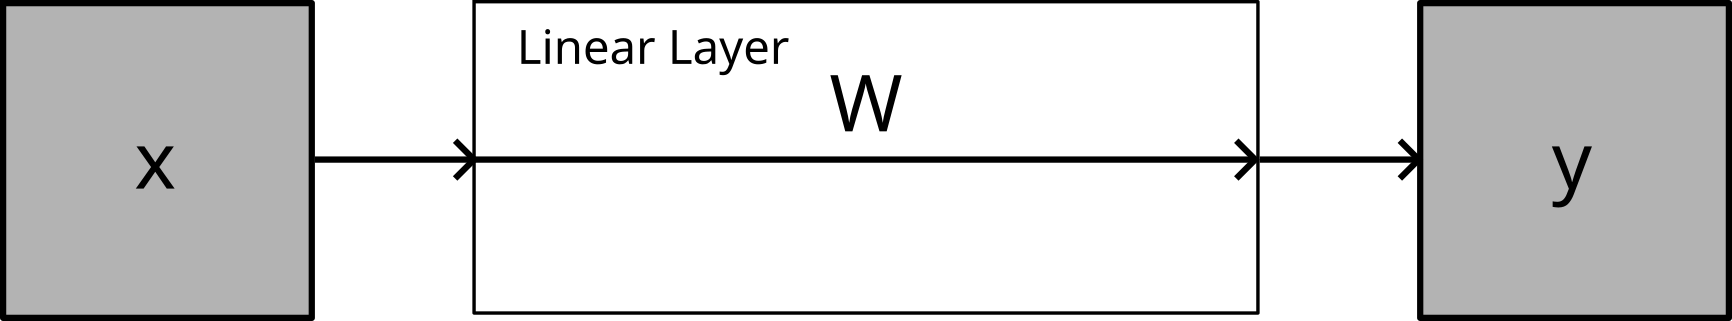
\includegraphics[width=\textwidth]{contents/Basics/linear.png}
    \caption{Illustration of the internal behavior of a linear layer.}
    \label{fig:linear-layer}
\end{figure}

 This relationship is graphically illustrated in Figure \ref{fig:linear-layer}.

\section{Recurrent}
\label{sect:rnn}

Recurrent models, specifically \gls{rnn}, are designed to handle sequential data effectively. Unlike linear models, \glspl{rnn} have the capability to retain information from previous inputs, making them well-suited for tasks involving \gls{ts} data, \gls{nlp}, and other domains where context is important.

\glspl{rnn} maintain a hidden state, which acts as the memory of the cell. It is updated at each time step using the current input and the previous hidden state. This allows RNNs to capture temporal dependencies and patterns in sequential data. Due to their recurrent nature, they can handle varying sequence lengths unlike linear layers. Figure \ref{fig:rnn} illustrates the internal behavior of an \gls{rnn}, highlighting how these models process and retain sequential information. The recurrent update of the hidden state \( h_t \) and output \( y_t \) at time step \( t \) in an RNN is defined as:

\begin{equation}
    h_t = \sigma(W_{hh} h_{t-1} + W_{xh} x_t + b_h) 
\end{equation}

\begin{equation}
    y_t = W_{hy} h_t + b_y 
\end{equation}

where \( x_t \) is the input at time step \( t \), \( W \) are the weight matrices, \( b \) are the biases, and \( \sigma \) is an activation function, typically a non-linear function like \gls{tanh} or \gls{relu}. The initial hidden state \( h_0 \) is typically initialized to zeros (\( h_0 = \mathbf{0} \)). Sigma is typically a non-linear function, such as sigmoid or \gls{tanh}, chosen for its ability to prevent saturation at extreme values and introduce non-linear behavior. The reason for this choise lies in the saturation of extreme values and providing non-linear behavior. 

Although \glspl{rnn} are appealing due to their ability to handle sequential data, they suffer from drawbacks. One major issue is the vanishing and exploding gradients problem, which causes the model to lose information over time. \gls{lstm} (see Section \ref{sect:lstm}) and \gls{lmu} (see Section \ref{sect:lmu}) are designed to mitigate this issue. Another drawback of \glspl{rnn} is their slow training times. Transformer models (see Section \ref{sect:trafo}) address this by introducing attention heads, which enables training parallelism and also eliminates the \gls{vgp}.

\todo{bigger font}
\begin{figure}[t]
    \centering
    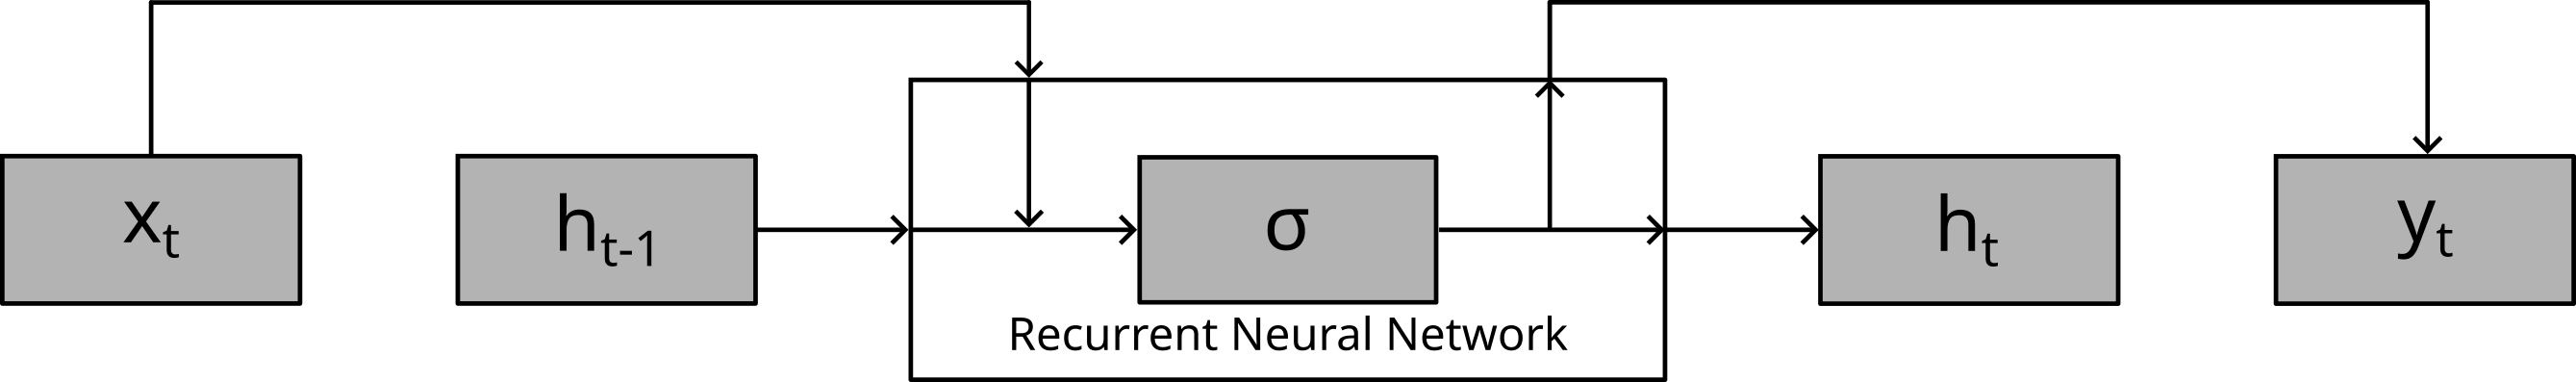
\includegraphics[width=\textwidth]{contents/Basics/rnn_flat.png}
    \caption{Illustration of the internal behavior of a Recurrent Neural Network (RNN).}
    \label{fig:rnn}
\end{figure}

\subsection{Long Short-Term Memory}
\label{sect:lstm}
The \gls{lstm} is a well-established state-of-the-art model in various machine learning applications. It addresses the \gls{vgp} through several gating mechanisms. The \gls{lstm} introduces three primary gates: the input gate, the output gate, and the forget gate. In addition, the cell state is updated by the cell gate mechanism, which plays a distinctive role in integrating new information. Each gate and the cell state work together to control the internal behavior of the modified \gls{rnn} cell. 

The forget gate regulates the flow of information from previous hidden and cell states. The input gate filters essential information from new input data, while the output gate selects pertinent output information. The cell gate, while not traditionally grouped with the primary gates, updates the cell state by integrating filtered new information.

Figure \ref{fig:lstm} illustrates the internal behavior of the \gls{lstm}, depicting how these gates and the cell state interact within the network. Additionally, the following equations define the version of the \gls{lstm} used in the Pytorch Documentation \cite{lstm-pytorch2} and also in :

\begin{equation}
    i_t = \sigma(W_{xi} x_t + W_{hi} h_{t-1} + b_{i})
\end{equation}
\begin{equation}
    f_t = \sigma(W_{xf} x_t + W_{hf} h_{t-1} + b_{f})
\end{equation}
\begin{equation}
    g_t = \tanh(W_{xg} x_t + W_{hg} h_{t-1} + b_{g})
\end{equation}
\begin{equation}
    o_t = \sigma(W_{xo} x_t + W_{ho} h_{t-1} + b_{o})
\end{equation}
\begin{equation}
    c_t = f_t \odot c_{t-1} + i_t \odot g_t
\end{equation}
\begin{equation}
    h_t = o_t \odot \tanh(c_t)
\end{equation}

In these equations, \(i_t\) represents the input gate activation at time step \(t\), while \(f_t\) denotes the forget gate activation at the same time step. The candidate cell state is captured by \(g_t\), and the output gate activation is represented by \(o_t\). The cell state at time step \(t\) is denoted as \(c_t\), and the hidden state as \(h_t\). The input at time step \(t\) is indicated by \(x_t\). The functions \(\sigma\) and \(\tanh\) refer to the sigmoid and \gls{tanh} activation functions, respectively, with \(\odot\) symbolizing element-wise multiplication.

\todo{replace mult with $\odot$ in Figure \ref{fig:lstm}}
\begin{figure}[t]
    \centering
    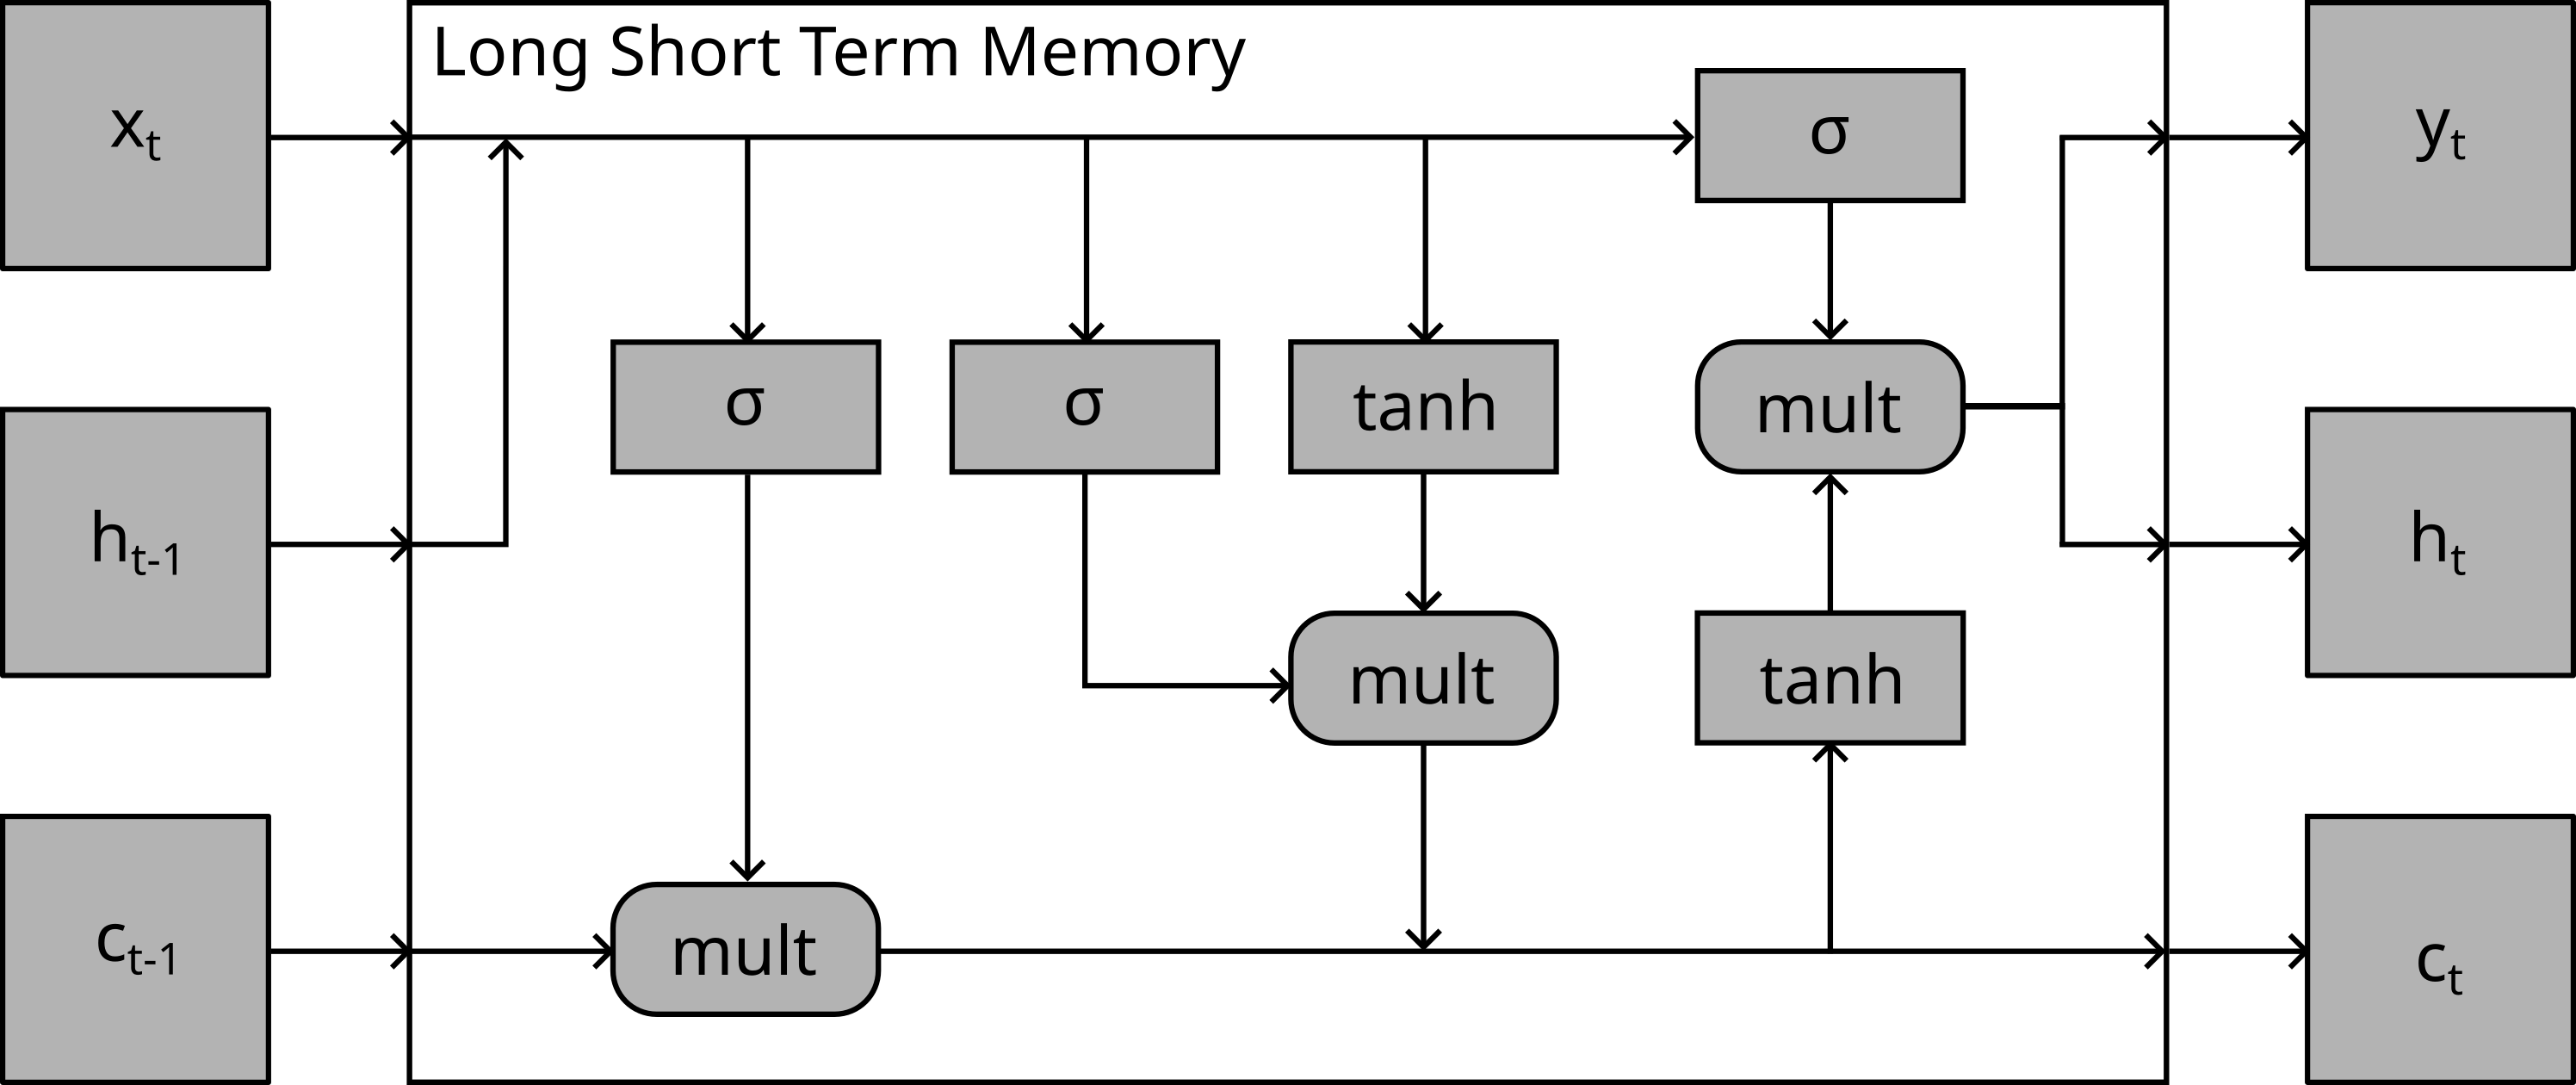
\includegraphics[width=\textwidth]{contents/Basics/lstm.png}
    \caption{Illustration of the internal behavior of the LSTM.}
    \label{fig:lstm}
\end{figure}


\subsection{Legendre Memory Unit}
\label{sect:lmu}

A novel gateless approach to address gradient vanishing was proposed by Voelker et al. \cite{lmu}. They introduced a method to emulate behaviors observed in the hippocampus, striatum, and cortex of the brain. Similar to these structures, the \gls{lmu} filters information continuously over time. It is claimed to preserve more information over longer durations than \glspl{lstm}, making it a promising alternative layer.

To understand the operation of \gls{lmu}, familiarity with \glspl{lp} is essential. \glspl{lp} are employed to enable the memory state of \gls{lmu} to retain information across extended periods. This requires using an orthogonal polynomial basis. Voelker et al. chose \glspl{lp} because they allow the memory state to be decomposed in a unique way, efficiently capturing long-term dependencies. They approximate the continuous-time delay \( F(s) = e^{-\theta s} \) with a window length \( \theta \) and Laplacian frequency \( s \) using the following ordinary differential equation:

\begin{equation}
\label{eq:ode_approx}
    \theta \dot{m}(t) = Am(t) + B(t)u(t)
\end{equation}

Here, \( m \in \mathbb{R}^d \) (with \( d \) as the memory size) represents the memory state, and \( u \in \mathbb{R} \) is the input, represented in terms of \glspl{lp}. Specifically, it involves sliding windows represented by \glspl{lp} up to degree \( d-1 \). The matrices \( A \in \mathbb{R}^{d \times d} \) and \( B \in \mathbb{R}^{d} \) in Equation \eqref{eq:ode_approx} are defined as:

\begin{equation}
\label{eq:a_bar}
    A = [a]_{ij}, \quad a_{ij} = \begin{cases}
    -1 & \text{if } i < j \\
    (-1)^{i-j+1} & \text{if } i \geq j
    \end{cases}
\end{equation}
\begin{equation}
\label{eq:b_bar}
    B = [b]_i, \quad b_i = (2i + 1)(-1)^i, \quad i, j \in [0, d-1]
\end{equation}

The equation \eqref{eq:ode_approx} is discretized as:

\[
m_t = \bar{A}m_{t-1} + \bar{B}u_t
\]

To achieve this, the continuous matrices \( A \) and \( B \) are discretized to obtain \( \bar{A} \) and \( \bar{B} \). Voelker et al. suggested using methods like Euler's method or \gls*{zoh} for sufficiently small \( \theta \). Algorithm \ref{alg:ssm} outlines the process to derive \( \bar{A} \) and \( \bar{B} \) in pseudocode for clarity. Additionally, Gosalci et al. \cite{gosalci} provided a comprehensive summary of the derivation of all functions described in this chapter.


\begin{algorithm}[H]
\caption{StateSpaceMatrices}
\label{alg:ssm}
\KwIn{$memory\_size$, $\theta$, $dt$}
$Q \gets \text{column vector of integers from } 0 \text{ to } memory\_size-1$\;
$R \gets \frac{1}{\theta}(2 Q + 1)$\;

$(i, j) \gets \text{create meshgrid from } Q$\;

$A \gets \text{zero matrix of size } (memory\_size, memory\_size)$\;
\For{each element $(i, j)$ in $A$}{
    \If{$i < j$}{
        $A[i, j] \gets -R[i, j]$\;
    }
    \Else{
        $A[i, j] \gets R[i, j] \cdot (-1)^{(i - j + 1)}$\;
    }
}

$B \gets \text{column vector of size } (memory\_size, 1)$\;
\For{each element $i$ in $B$}{
    $B[i] \gets R[i] \cdot (-1)^i$\;
}

$A\_discrete \gets dt \cdot A + I$\;
$B\_discrete \gets dt \cdot B$\;

\KwOut{$A\_discrete$, $B\_discrete$}
\end{algorithm}



The \gls{lmu} is defined as:
\begin{equation}
    u_t = e_x^T x_t + e_h^T h_{t-1} + e_m^T m_{t-1}
\end{equation}
\begin{equation}
    m_t = \Bar{A} m_{t-1} + \Bar{B} u_t
\end{equation}
\begin{equation}
    h_t = f(W_x x_t + W_h h_{t-1} + W_m m_t)
\end{equation}
In these equations, \(e_x \in \mathbb{R}^{\text{dim}(x),1}\) represents the input encoding vector, \(e_m \in \mathbb{R}^{d,1}\) is the memory encoding vector, and \(e_h \in \mathbb{R}^{n,1}\) denotes the hidden encoding vector. The weight matrices are defined as \(W_x \in \mathbb{R}^{\text{dim}(x),n}\) for the input, \(W_m \in \mathbb{R}^{d,n}\) for the memory, and \(W_h \in \mathbb{R}^{n,n}\) for the hidden state. The coefficients \(\Bar{A}\) and \(\Bar{B}\) are defined in Equations \eqref{eq:a_bar} and \eqref{eq:b_bar}, respectively. The function \(f\) refers to any nonlinearity, such as sigmoid, tanh, or ReLU. The initial states \(h_0\) and \(m_0\) are typically initialized as zero vectors. Figure \ref{fig:lmu} shows the internal behavior of the LMU graphically.


\begin{figure}[t]
    \centering
    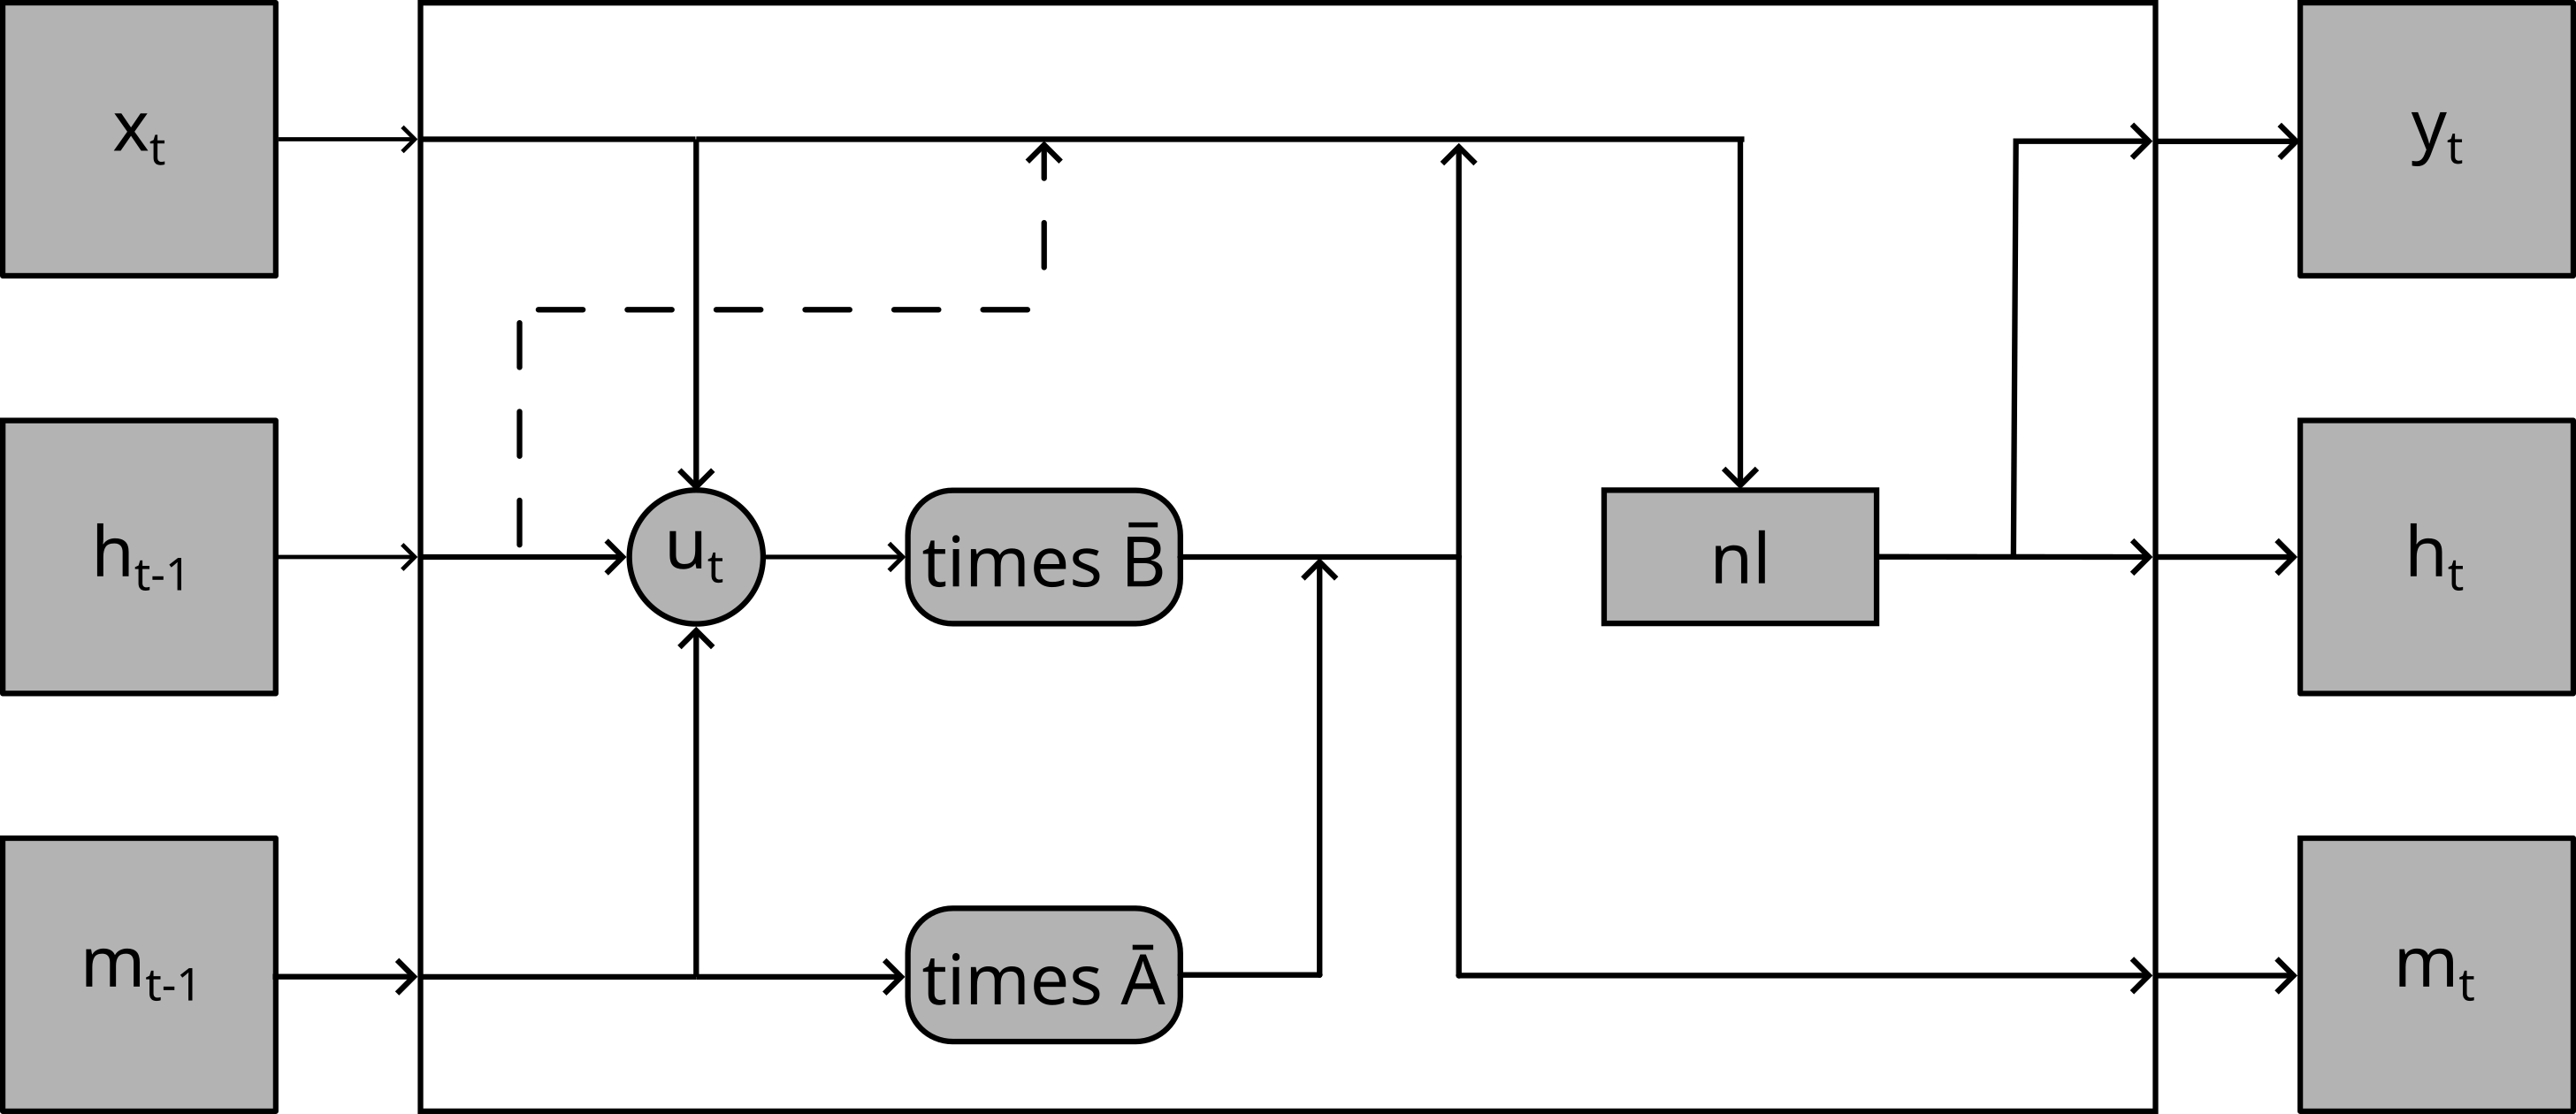
\includegraphics[width=\textwidth]{contents/Basics/lmu.png}
    \caption{Illustration of the internal behavior of the LMU. The dashed line is used to differentiate it from the solid lines it intersects.}    
    \label{fig:lmu}
\end{figure}


\section{Attention-Based Transformer}
\label{sect:trafo}
Despite the development of \gls{lstm} and \gls{lmu}, recurrent models still suffered from information leakage over time, necessitating a new approach. A novel advancement in \gls{nlp} is the use of attention-based models, particularly transformer models, which have become pivotal in the field. As of 2024, most \gls{sota} \glspl{llm}, such as OpenAI's GPT \cite{gpt} and Anthropic's Claude \cite{claude}, are closed-source models utilizing attention mechanisms. On the other hand, open-source alternatives include Meta's LLaMa and OPT \cite{llama,opt}, and Big Science's Bloom \cite{bloom}. Each of these models employs different approaches, making it unclear which architecture is the most promising for the task of predicting trajectories.

The original work by Vaswani et al. \cite{transformer} introduced a model comprising multiple encoder and decoder blocks. However, it was found that the decoder block was not suitable for this task. The decoder-only model generates outputs sequentially and aggregates predictions step-by-step, which can lead to cumulative errors through feedback mechanisms. This sequential generation process makes it prone to increasing inaccuracies over time. Consequently, an encoder-only transformer, such as Devlin et al.'s BERT \cite{bert}, is preferred for this task. The encoder-only transformer processes the entire input at once and generates the output in one step, avoiding the error propagation issues seen in decoder-only models. It consists of a positional encoder (see Section \ref{sec:posenc}) followed by multiple sequential encoder blocks (see Section \ref{sec:enc_block}) and concludes with mini-batch normalization (see Section \ref{sec:laynorm}). This structure is illustrated in Figure \ref{fig:transformer}.

\begin{figure}[t]
    \centering
    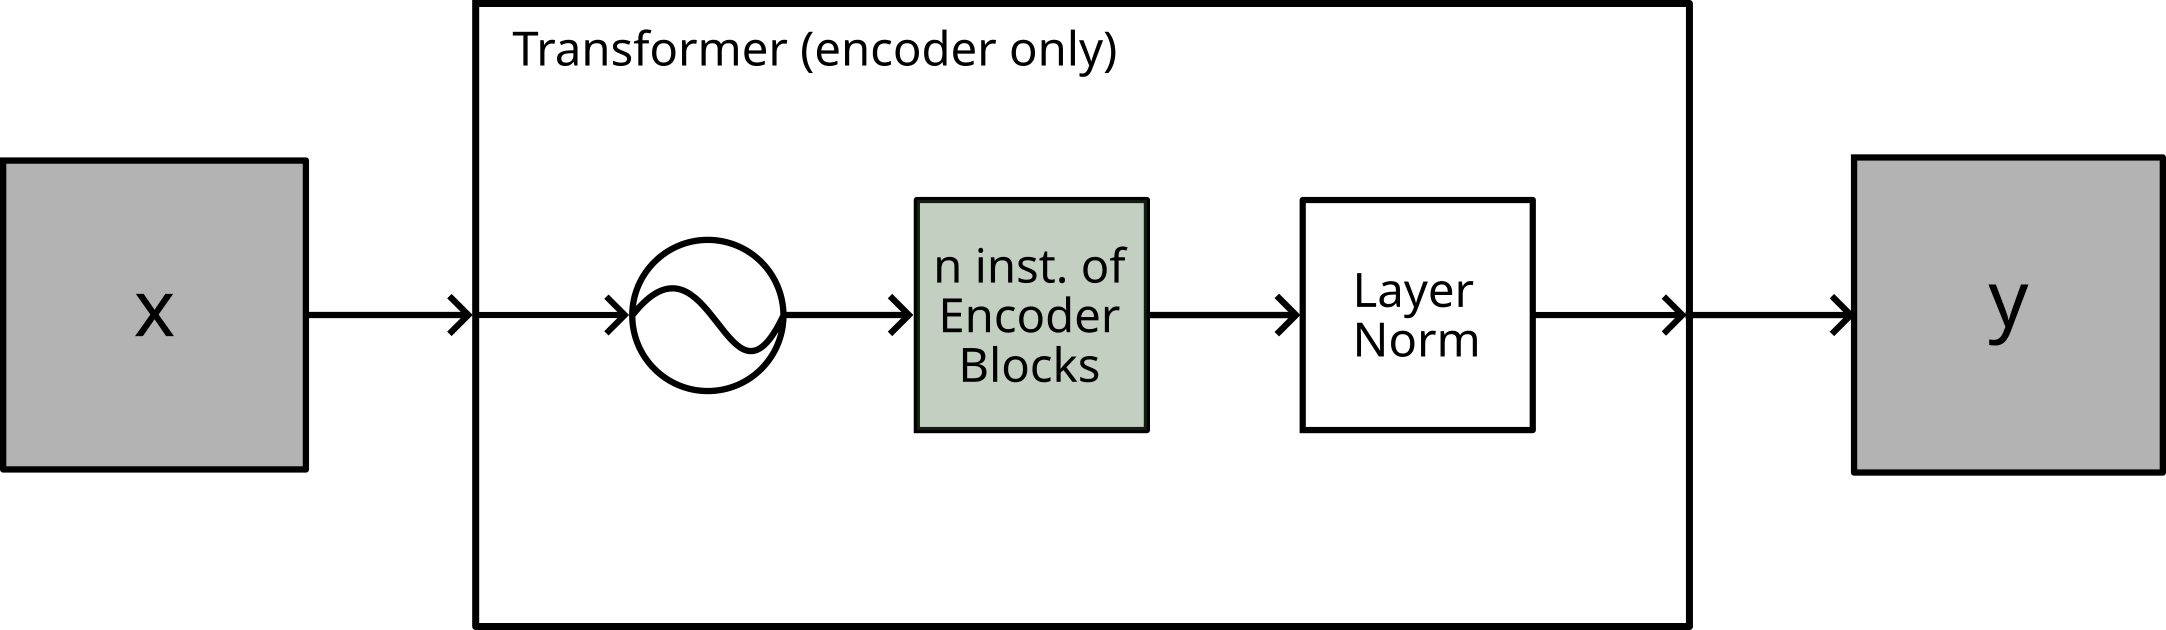
\includegraphics[width=\textwidth]{contents/Basics/transformer.png}
    \caption{Illustration of the internal behavior of the Transformer.}
    \label{fig:transformer}
\end{figure}

Figure \ref{fig:transformer} provides a high-level view of the Transformer model. The subsequent sections will delve into specific components of the transformer, each accompanied by a detailed illustration and pseudocode.

\subsection{Positional Embeddings}
\label{sec:posenc}
In transformer models, positional embeddings are crucial for incorporating the order of the sequence into the model. Unlike \glspl{rnn} that process sequences step-by-step, transformers process the entire sequence simultaneously. Therefore, they need a mechanism to inject information about the position of each token in the sequence, enabling the model to understand the order and temporal relationships between tokens.

\subsubsection{Importance of Positional Embeddings}

Positional embeddings provide a sense of order to the model, allowing it to distinguish between tokens at different positions in the sequence. They help the model capture temporal dependencies, which is particularly important for sequential data such as text or audio. By knowing the position of each token, the model can better understand the context in which each token appears, improving its ability to generate accurate and contextually relevant outputs.

\subsubsection{Sinusoidal Positional Embeddings}

The original transformer model by Vaswani et al. \cite{transformer} introduces sinusoidal positional embeddings. These embeddings use sine and cosine functions of different frequencies to encode the position of each token in a sequence. The positional encoding for a position $pos$ and dimension $i$ is defined as follows:

\begin{minipage}{\textwidth}
\begin{equation}
\text{PE}_{(pos, 2i)} = \sin\left(\frac{pos}{10000^{\frac{2i}{d_{\text{model}}}}}\right)
\end{equation}
\begin{equation}
\text{PE}_{(pos, 2i+1)} = \cos\left(\frac{pos}{10000^{\frac{2i}{d_{\text{model}}}}}\right)
\end{equation}
\end{minipage}

where $pos$ is the position and $i$ is the dimension index. This approach allows the model to easily learn to attend by relative positions.

\subsubsection{Convolutional Layer as Positional Embedding}

In their work, Baevski et al. \cite{baevski2020} use a convolutional layer instead of sinusoidal positional embeddings. A convolutional layer is utilized for its ability to effectively capture temporal dependencies, which is essential for understanding the structure and content of sequential data such as speech. The convolutional layer is effective at extracting local temporal features, crucial for capturing low-level patterns in the data.

Moreover, rather than using fixed positional embeddings that encode absolute positional information, Baevski et al. employ a convolutional layer as a relative positional embedding. This approach allows the model to encode relative positional information, which can be more flexible and beneficial for various tasks. The output of the convolution is followed by a \gls{gelu} activation and then added to the inputs, followed by layer normalization.

For tasks involving the prediction of trajectories in complex scenes, such as \gls{nba} games or soccer matches, a convolutional layer can offer several advantages. By providing a hierarchical representation of the input, the model can capture both local and broader temporal contexts. This representation can be particularly beneficial for understanding the dynamic and intricate patterns in sports trajectories, where both short-term movements and longer-term strategies need to be considered.

Furthermore, the convolutional layer can reduce the length of the input sequence through pooling or strided convolutions, which reduces computational complexity for the subsequent transformer layers. This can be advantageous in handling the extensive data generated in sports scenarios, allowing for more efficient and scalable model training and inference.



\subsection{Encoder Block}
\label{sec:enc_block}
The Transformer model primarily consists of encoder blocks. Each encoder block processes the input through a series of layers, including \gls{mha} and \glspl{ffn}. The detailed structure of an encoder block is shown in Figure \ref{fig:encoder_block}. The pseudocode for the encoder block forward pass is provided in Algorithm \ref{alg:encoder_layer}.

\begin{figure}[t]
    \centering
    \begin{minipage}{\textwidth}
        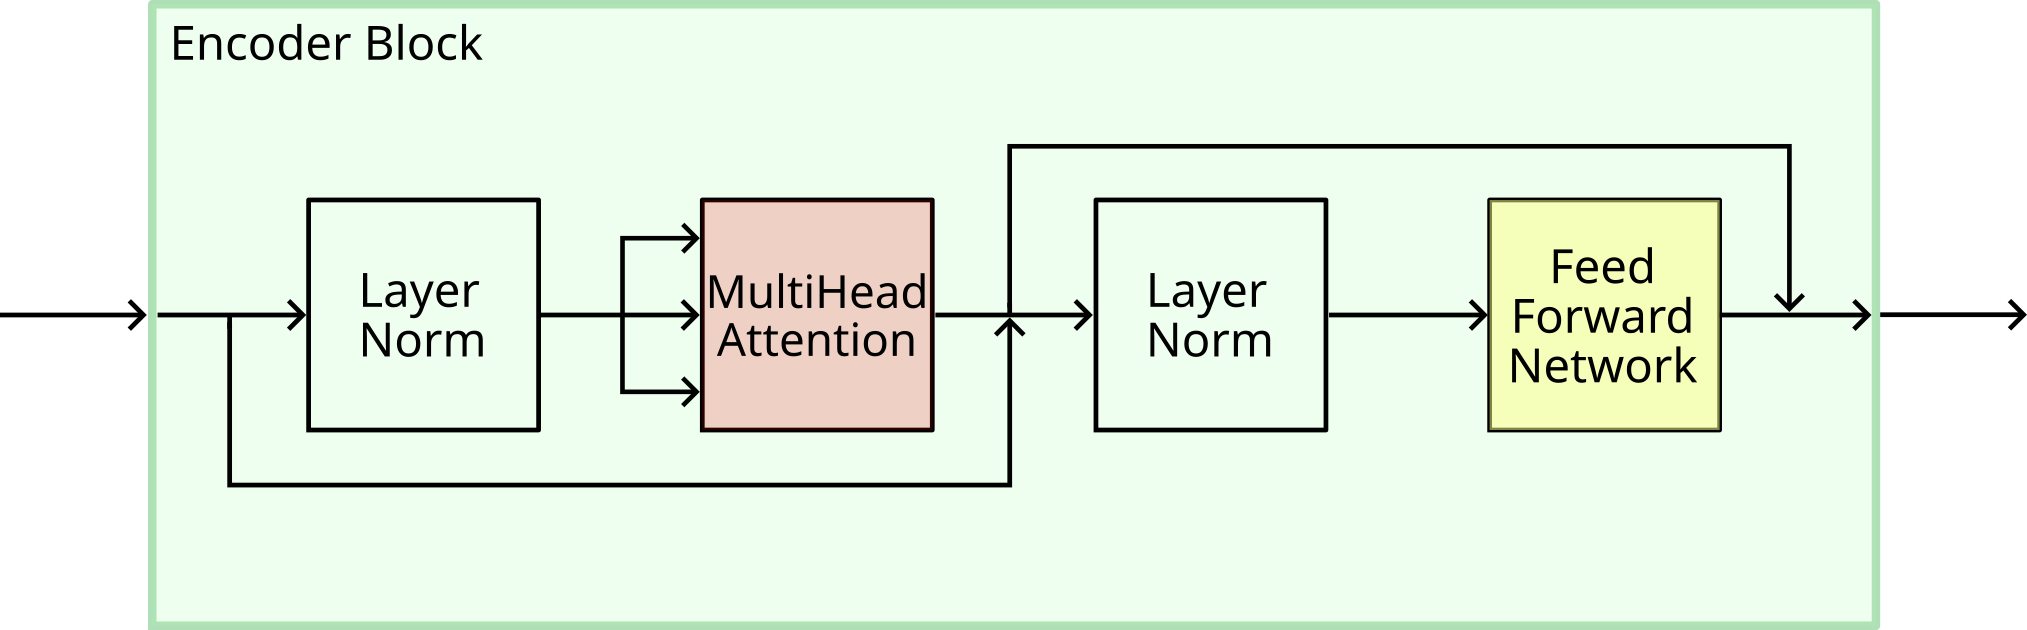
\includegraphics[width=\textwidth]{contents/Basics/encoder_block.png}
        \caption{Zoom into the encoder block of the Transformer.}
        \label{fig:encoder_block}
    \end{minipage}
    \vspace{-1em} % Adjust vertical space if necessary
\end{figure}

\todo{Make colors less saturated in Figure \ref{fig:encoder_block}.}

\begin{figure}[t]
    \centering
    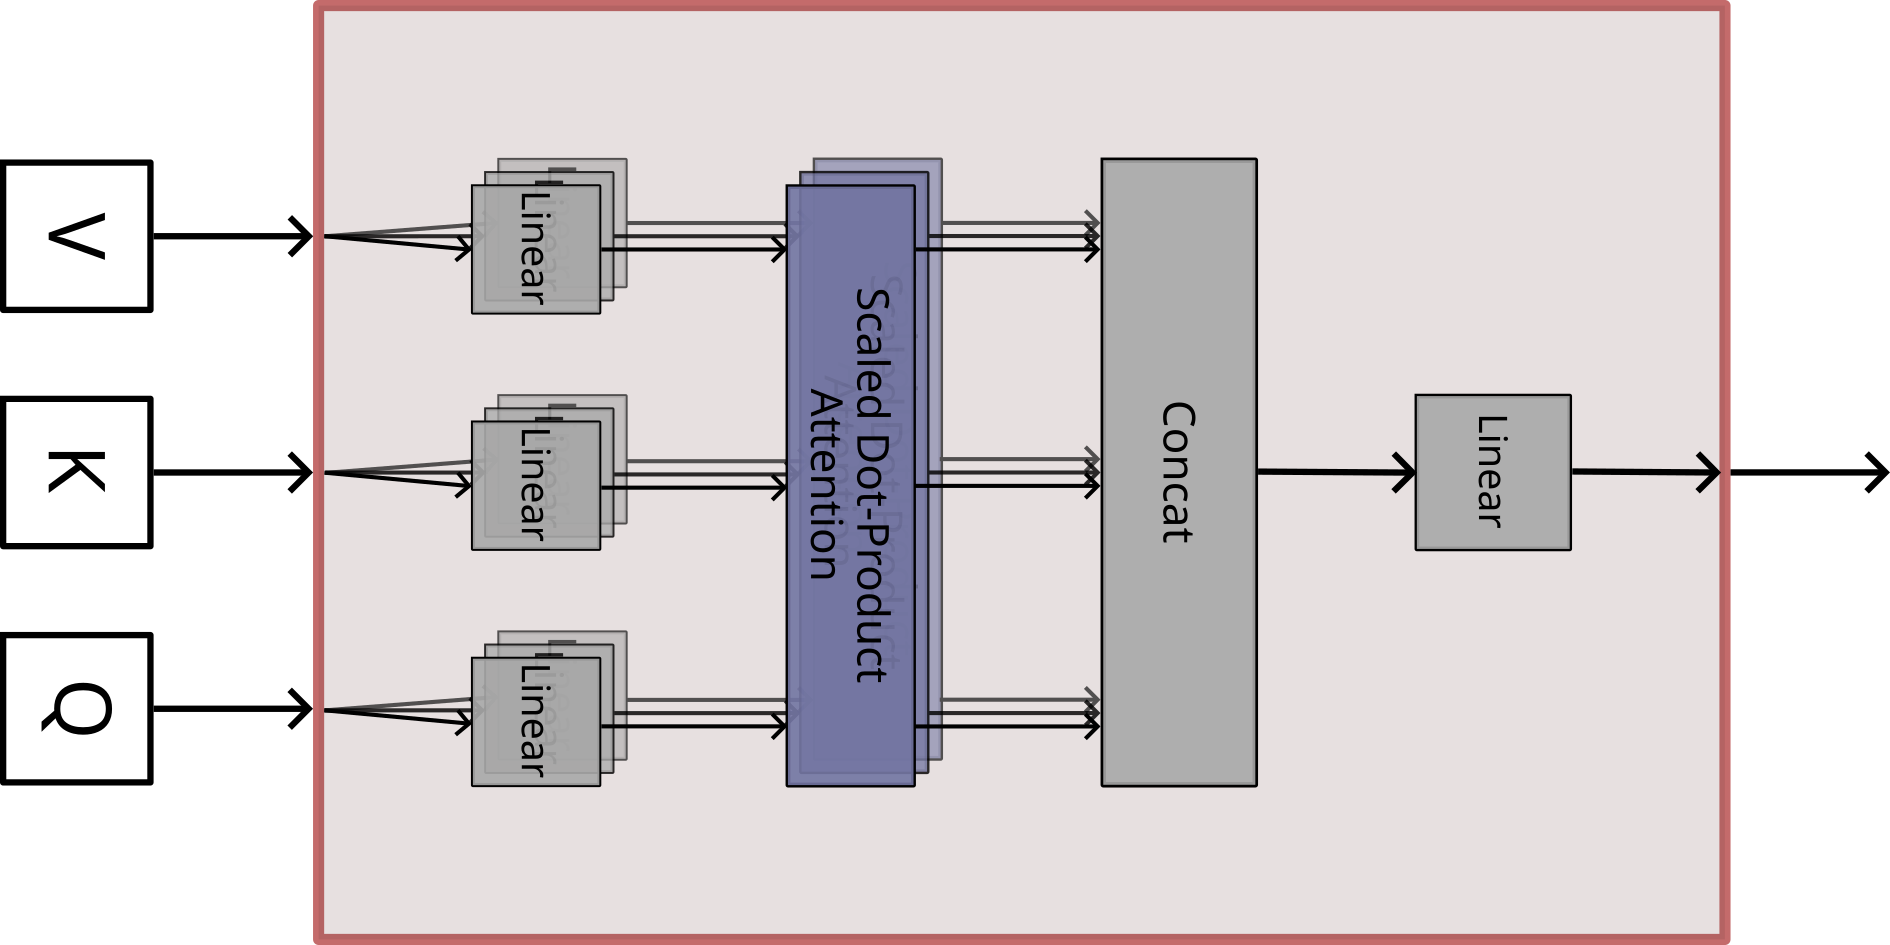
\includegraphics[width=\textwidth]{contents/Basics/MHA.png}
    \caption{Zoom into the Multi-Head Attention.}
    \label{fig:multihead_attention}
\end{figure}

\begin{algorithm}[H]
\caption{EncoderLayer Forward Pass}
\label{alg:encoder_layer}
\KwIn{$x$, $encoder\_mask$}
$c1 \gets \text{LayerNorm}_1(x)$\;
$c2 \gets \text{MultiHeadAttention}(c1, c1, c1, encoder\_mask)$\;
$c3 \gets c2 + x$\;
$c4 \gets \text{LayerNorm}_2(c3)$\;
$c5 \gets \text{PositionwiseFFN}(c4)$\;
\KwOut{$c3 + c5$}
\end{algorithm}


In the encoder block, the input $x$ first passes through a Layer Normalization step (see Section \ref{sec:laynorm}). The normalized input, denoted as $c1$, then goes through the \gls{mha} mechanism which is detailed in Section \ref{sec:mha}. The resulting $c2$ is added to the input vector $x$ to get $c3$. $c4$ is then fed through a second Layer Normalization, and after being processed by the \gls{ffn} (see Section \ref{sec:ffn}), we obtain $c5$. The final output of the encoder block is $c3 + c5$.


\subsection{Multi-Head Attention}
\label{sec:mha}
\gls{mha} is a key component of the transformer model, enabling it to focus on different parts of the input sequence simultaneously. In this mechanism, the input is split into multiple heads of size $d_k$. Each head is processed through a linear layer and then fed into the Scaled Dot-Product Attention. The outputs from all heads are concatenated and processed through another linear layer. This detailed structure is shown in Figure \ref{fig:multihead_attention}.

\begin{algorithm}[H]
\caption{Multi-Head Attention Forward Pass}
\label{alg:multihead_attention}
\KwIn{Queries, Keys, Values, Mask}
$d_k \gets \frac{n\_out}{n\_heads}$\;
Queries' $\gets \text{Linear}(\text{Queries})$\;
Keys' $\gets \text{Linear}(\text{Keys})$\;
Values' $\gets \text{Linear}(\text{Values})$\;
Queries $\gets \text{SplitIntoHeads}(\text{Queries', }d_k)$\;
Keys $\gets \text{SplitIntoHeads}(\text{Keys', }d_k)$\;
Values $\gets \text{SplitIntoHeads}(\text{Values', }d_k)$\;
$x \gets \text{ScaledDotProductAttention}(\text{Queries, Keys, Values, Mask})$\;
$x \gets \text{Reshape}(x)$\;
$x \gets \text{Linear}(x)$\;
\KwOut{$x$}
\end{algorithm}

The pseudocode for the \gls{mha} forward pass is provided in Algorithm \ref{alg:multihead_attention}. It illustrates the process of splitting the input into Queries, Keys, and Values heads. These are then processed through the \gls{sdpa} (see Section \ref{sec:sdpa}). After reshaping, the output is obtained by applying a final linear layer.


\subsection{Scaled Dot-Product Attention}
\label{sec:sdpa}

\begin{figure}[t]
    \centering
    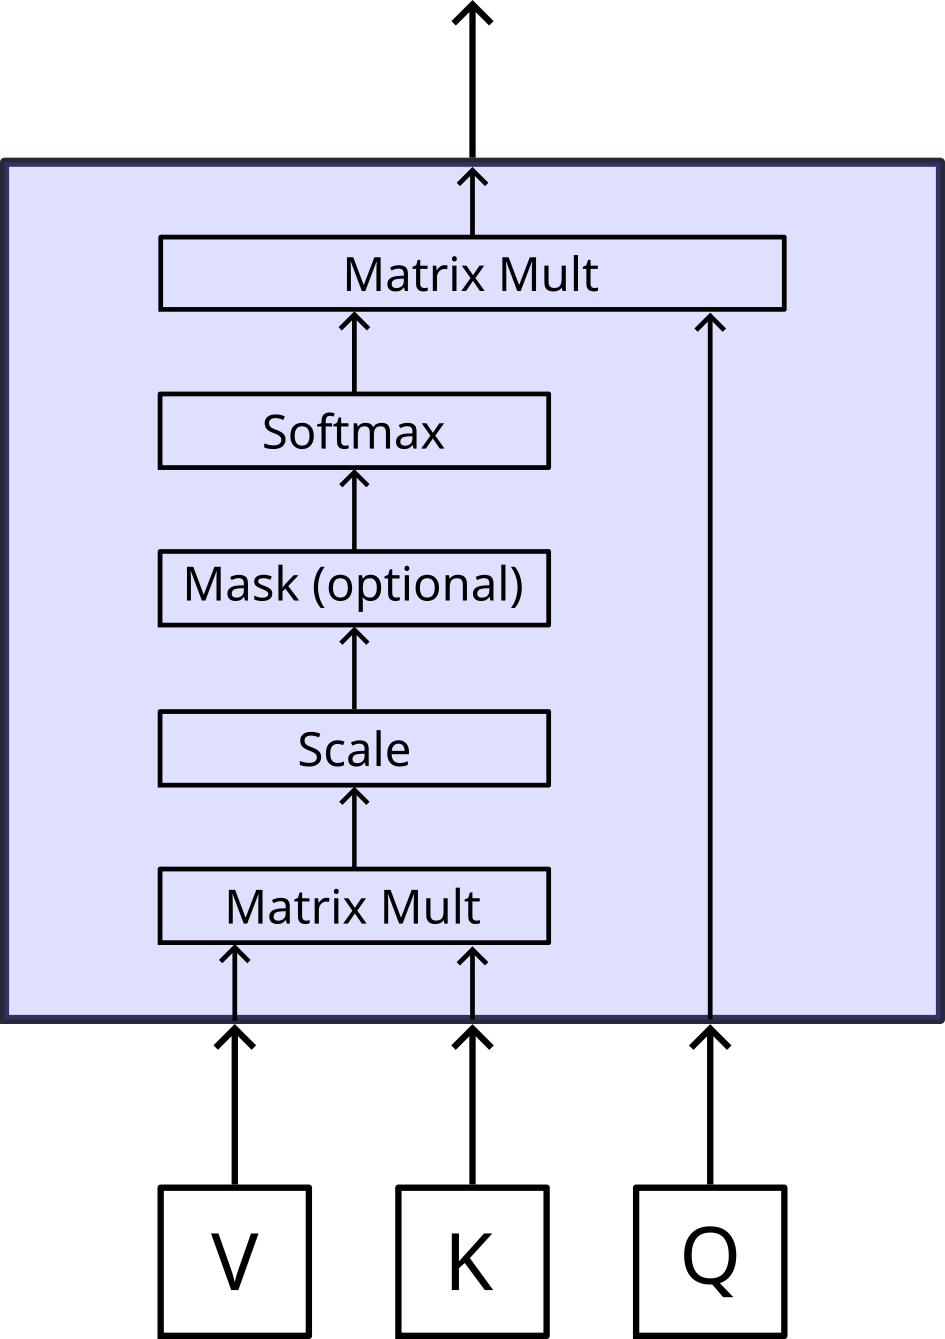
\includegraphics[width=0.5\textwidth]{contents/Basics/scaled_dot_product.png}
    \caption{Zoom into the Scaled Dot-Product Attention.}
    \label{fig:scaled_dot_product}
\end{figure}
Within the \gls{mha} mechanism, Scaled Dot-Product Attention is essential for computing the attention scores between queries and keys. These scores are then used to weigh the values. An optional encoder mask can be applied to prevent certain positions from attending to others, though this feature is not used in this work. A detailed view of Scaled Dot-Product Attention is shown in Figure \ref{fig:scaled_dot_product}.

The function of Scaled Dot-Product Attention is mathematically represented as:

\begin{equation}
\text{Attention}(Q, K, V) = \text{softmax}\left(\frac{QK^T}{\sqrt{d_k}}\right)V
\end{equation}

where $Q$, $K$, and $V$ are the query, key, and value matrices, respectively, and $d_k$ is the dimension of the keys.

Softmax is a function used to convert the attention scores into a probability distribution. It ensures that the weights assigned to each key sum to one, allowing the model to interpret these weights as probabilities. The Softmax function is defined as:

\begin{equation}
\text{softmax}(z_i) = \frac{\exp(z_i)}{\sum_{j} \exp(z_j)}
\end{equation}

where \( z_i \) represents the score for the \( i \)-th key, and the denominator sums over all scores to normalize them.

The algorithm for Scaled Dot-Product Attention proceeds as follows: First, the attention scores are computed by taking the dot product of the query matrix $Q$ and the transpose of the key matrix $K$, and then scaling these scores by \( \sqrt{d_k} \). This scaling is crucial to avoid excessively large values in the dot product. The scaled scores are then passed through the Softmax function to obtain normalized attention weights. If an encoder mask is used, it adjusts the attention scores accordingly, though this is not applicable in the current work. Finally, these attention weights are applied to the value matrix $V$ to produce the weighted output. This mechanism enables the model to focus on different parts of the input sequence based on the computed attention weights.


\subsection{Positionwise Feed-Forward Network}
\label{sec:ffn}
After the attention mechanism, the data passes through a \gls{ffn}, which applies a fully connected network to each position independently and identically. The \gls{ffn} consists of two linear layers with a ReLU activation function in between, followed by a dropout layer. The detailed structure of the \gls{ffn} is shown in Figure \ref{fig:ffn} and the pseudocode is provided as Algorithm \ref{alg:ffn2}.

Finally, each encoder block concludes with another Layer Normalization step, ensuring stable and normalized data propagation.

\begin{figure}[t]
    \centering
    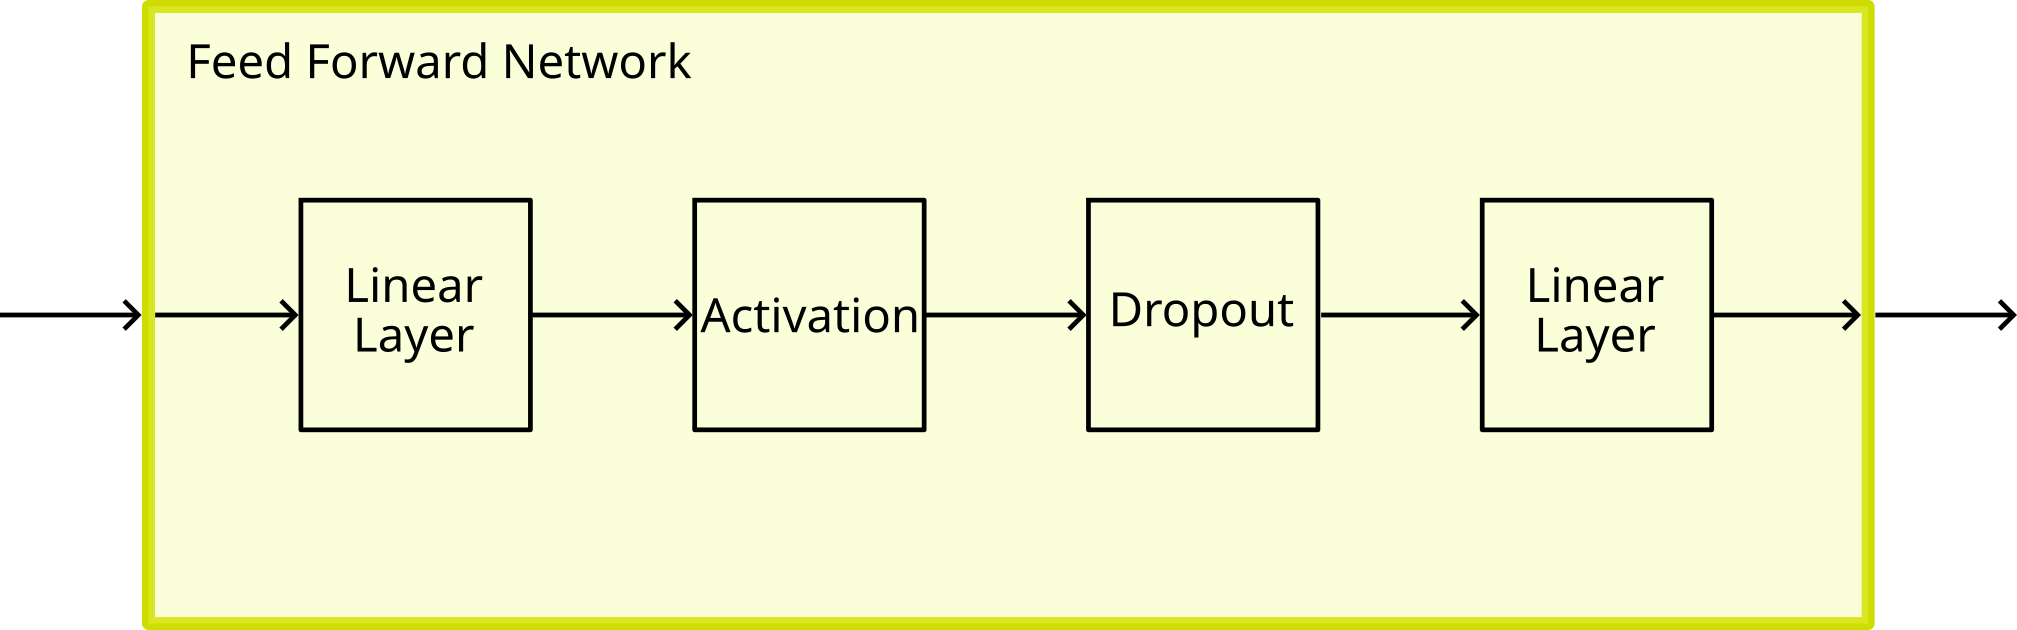
\includegraphics[width=\textwidth]{contents/Basics/FeedforwardNetwork.png}
    \caption{Zoom into the Feedforward Mechanism of the encoder.}
    \label{fig:ffn}
\end{figure}

\subsection{Layer Normalization}
\label{sec:laynorm}
Layer normalization is applied to both the input and output of the attention and feed-forward layers. It normalizes the input tensor across the features and is defined as:

\begin{equation}
\label{eq:layernorm}
    y = \frac{x - \text{E}[x]}{\sqrt{\text{Var}[x] + \epsilon}} \cdot \gamma + \beta
\end{equation}

In this equation, \( \text{E}[x] \) represents the mean of the input tensor, while \( \text{Var}[x] \) denotes its variance. The term \( \epsilon \) is a small constant added to the variance to ensure numerical stability. The parameters \( \gamma \) and \( \beta \) are learnable, with \( \gamma \) serving as a scale parameter that adjusts the normalized output, and \( \beta \) acting as a shift parameter that offsets the normalized output.

\begin{algorithm}[H]
\caption{Positionwise Feed-Forward Network Forward Pass}
\label{alg:ffn2}
\KwIn{$x$}
$x \gets \text{Linear}_1(x)$\;
$x \gets \text{ReLU}(x)$\;
$x \gets \text{Dropout}(x)$\;
$x \gets \text{Linear}_2(x)$\;
\KwOut{$x$}
\end{algorithm}


\subsection{Learning Rate-Warm-Up Scheduler}
\label{sec:scheduler}

Training transformer models requires careful selection of the optimizer and learning rate schedule to ensure stable and efficient learning. The Adam \cite{adam} optimizer is commonly used due to its ability to adjust learning rates dynamically for each parameter based on gradient estimates. However, transformers are particularly sensitive to the learning rate, especially in the early stages of training.

To address this, a warm-up phase is introduced, where the learning rate starts low and increases gradually. This prevents large gradient updates from destabilizing the training process in the beginning. The learning rate schedule typically follows the formula proposed by Vaswani et al. \cite{transformer}:

\begin{equation}
\text{LR}(step) = d_{\text{model}}^{-0.5} \cdot \min(step^{-0.5}, step \cdot warmup\_steps^{-1.5})
\end{equation}

Here, $d_{\text{model}}$ is the model’s dimensionality, and $warmup\_steps$ determines the length of the warm-up phase. After the warm-up, the learning rate decreases based on the inverse square root of the step count. This approach ensures that the model trains smoothly, avoiding instability, and achieves better performance by allowing the optimizer to adapt gradually.

For instance, the \gls{llama} \cite{llama} model uses the AdamW optimizer with a linear learning rate warm-up schedule of 2,000 \(warmup\_steps\). Similarly, the \gls{opt} \cite{opt} model also employs AdamW with a linear warm-up of 2,000 \(warmup\_steps\). \gls{bert} \cite{bert} utilizes the Adam optimizer with a warm-up phase of 10,000 \(warmup\_steps\), while \gls{bloom} \cite{bloom} adopts Adam with a cosine learning rate decay schedule.


\section{BitNet: 1-Bit Transformer}
\label{sect:bitnet}

BitNet, as introduced by Wang et al. \cite{BitNet2023}, innovatively replaces the traditional linear layers of the Transformer model with BitLinear layers. This modification involves reducing the precision of weights and activations to 1 bit, thereby significantly decreasing computational and memory requirements. Unlike traditional transformers, BitNet can leverage higher learning rates, enhancing training efficiency.

The core of BitNet's architecture is the BitLinear layer, which employs binary weights and activations. During forward propagation, the computations are performed using bitwise operations, which are inherently faster and more efficient than standard floating-point operations. The output of a BitLinear layer is expressed as:
\[
\mathbf{y} = \text{sign}(\mathbf{W}\mathbf{x} + \mathbf{b})
\]
where \(\mathbf{W}\) and \(\mathbf{x}\) represent the binary weight matrix and input vector, respectively, and \(\mathbf{b}\) denotes the bias term.

The primary advantage of BitNet lies in its substantial reduction of memory and energy consumption. This is particularly beneficial in high dynamic environments where predicting trajectories demands efficient and scalable models. Compared to traditional Transformers, \gls{lstm}, and LMUs, BitNet maintains the effectiveness of the Transformer architecture while optimizing resource usage, leading to a promising modification. Additionally, BitNet allows for larger learning rates compared to Transformers and does not require a warmup phase.

\section{TimeGPT}
\label{sect:timegpt}

TimeGPT was initially identified as a promising tool for time series forecasting due to its precompiled Transformer model specifically designed for time series analysis. The initial availability of TimeGPT as a free resource made it an attractive option for leveraging advanced Transformer-based techniques without financial costs.

However, during the course of the research, TimeGPT transitioned to a subscription-based model, requiring payments of \$99.00 for basic access and \$399.00 for additional support services. This change in the pricing structure significantly impacted its suitability for continued use in the research. The introduction of these fees conflicted with the objective of maintaining a cost-effective and financially independent research framework. Additionally, reliance on a subscription model raised concerns about potential financial benefits accruing to the service provider from the research activities.

Furthermore, there was a strong preference for utilizing and developing open-source solutions. Open-source tools provide transparency, reproducibility of results, and eliminate financial constraints on research activities. This approach ensures the integrity and independence of the research process.

In light of these considerations, TimeGPT was excluded from the research framework. The decision to exclude TimeGPT was motivated by the need to avoid endorsing proprietary software and to prioritize tools that do not benefit financially from the research efforts. The focus was thus redirected towards self-trained models and freely available resources, ensuring that the study remains unbiased and independent.

In conclusion, although TimeGPT initially appeared to be a viable option due to its advanced capabilities and initial free access, the subsequent change in its accessibility and associated costs necessitated its exclusion. This decision underscores the commitment to open-source methodologies and the financial independence of the research.

\section{Performance Measurement}
\label{sec:performance}
\gls{mse} quantifies the average squared difference between predicted and true values. It is defined as:
\begin{equation}
\text{MSE} = \frac{1}{n \cdot m} \sum_{i=1}^n \sum_{j=1}^m \left( \hat{y}_{i,j} - y_{i,j} \right)^2
\end{equation}
where \(\hat{y}_{i,j}\) and \(y_{i,j}\) are the predicted and actual values, respectively, for the \(i\)-th sample and \(j\)-th feature, \(n\) is the number of samples, and \(m\) is the number of features. This meassurement is also used to train the models.

\section{Transfer Learning}
\label{sect:transfer-learning}

\gls{tl} is a technique where knowledge acquired from training a model on one domain is utilized to enhance performance on a different, but related, domain. This method is especially valuable when the target domain has limited data or when it is impractical to train a model from scratch due to high computational costs.

The process of \gls{tl} involves several key steps. Initially, a model is pre-trained on a large and diverse dataset from a source domain. This source dataset allows the model to learn general features and patterns that are broadly applicable. Once pre-training is complete, the model undergoes fine-tuning on a new dataset from the target domain. This step adjusts the model's parameters to better align with the specific characteristics of the target data. Fine-tuning can either involve training the entire model or selectively adjusting certain layers, depending on the degree of similarity between the source and target domains. Finally, the performance of the fine-tuned model is evaluated to ensure that it effectively generalizes to the new domain and meets the desired performance criteria.

\gls{tl} has demonstrated significant effectiveness across various fields. In computer vision, for example, models pre-trained on large image datasets such as ImageNet have been successfully adapted for diverse tasks including object detection and medical image analysis \cite{pan2009survey, GoodBengCour16}. Similarly, in natural language processing, pre-trained models like BERT and GPT have been fine-tuned for specific tasks such as sentiment analysis and translation \cite{bert, radford2019language}.

In this research, \gls{tl} is utilized to investigate whether models trained on basketball data can be effectively adapted and fine-tuned for soccer data and vise versa. This approach aims to evaluate the generalizability of features learned from one sport to another and to assess how well pre-trained models can be adapted to new types of data.


\chapter{Method}
\label{chapt:method}

This Chapter outlines the methods and processes used to develop and evaluate the predictive models for player and ball movements in sports data. Section \ref{sec:idea_pipeline} introduces the overarching idea and the pipeline employed, setting the stage for the modeling approach. Section \ref{sec:preprocessing} details the data pre-processing techniques essential for preparing the raw input data for model training. Sections \ref{sec:main_proc} and \ref{sec:postprocessing} then delve into the specific models and post-processing techniques used to convert the model outputs into meaningful, real-world predictions.

\section{Idea and Pipeline}
\label{sec:idea_pipeline}
\begin{figure}[H]
    \centering
    \includesvg[width=1\linewidth]{contents//Basics/pipeline.svg}
    \caption{Overview of the predictive modeling pipeline for sports data.}
    \label{fig:pipeline}
\end{figure}
The primary objective of this thesis is to develop a robust pipeline for forecasting player movements in dynamic sports environments, such as basketball and soccer. Traditional methods, such as \glspl{kf} and \glspl{pf}, often fall short due to the complexity and nonlinearity of the data in these scenarios. This research aims to address these challenges by employing advanced \glspl{nn} capable of capturing temporal dependencies and intricate patterns in multivariate time series data. The proposed pipeline consists of three main stages:
\\ \\
\textbf{Pre-processing:} Transform raw data from all datasets into a unified structure. Additionally, the pre-processing step split the data into sliding windows for use in the main process. The process is described in Section \ref{sec:preprocessing}.
\\ \\
\textbf{Main-processing:} This stage encompasses training, validation, and testing of the model. Detailed steps for ensuring reproducibility are provided in Section \ref{sec:main_proc}.
\\ \\
\textbf{Post-processing:} The raw model outputs are refined to improve readability and interpretability. Section \ref{sec:postprocessing} details the main steps for converting the outputs into a more human-friendly format.

\section{Pre-processing}
\label{sec:preprocessing}

\begin{figure}
    \centering
    \includesvg[width=1\linewidth]{contents//Basics/block_plain.svg}
    \caption[Illustration of the rolling window process with colored windows and increased step size for clarity.]{Illustration of the rolling window process. Different sliding windows are highlighted using distinct colors: red, green, and blue, to differentiate between them. For illustration purposes, the step size is increased to 4, allowing for clearer visualization of the overlapping windows. Multiple trajectories are shown, with those in the background having reduced opacity and gradually fading out, creating a sense of depth as they move leftward and downward.}
    \label{fig:preprocessing}
\end{figure}

The first step of the pre-processing involves collecting all relevant data and transforming it into a unified structure. This process not only ensures consistency but also simplifies the main processing stage (refer to Section \ref{sec:main_proc}), as it requires consideration of only one unique data structure. The output of this pre-processing step is a 3D structure with the shape \texttt{[num\_timesteps, num\_objects, num\_features]} for each trajectory. Here, \texttt{num\_timesteps} corresponds to the duration of each trajectory, \texttt{num\_objects} represents all relevant entities in the scene—specifically, Team 1, followed by Team 2, the ball, Team 1's goal/basket, and Team 2's goal/basket—and \texttt{num\_features} denotes the attributes of that scene. Both datasets are sampled at 25 Hz, so the resulting dataset retains this sampling rate, with each trajectory reflecting 25 samples per second. In both the NBA and DFL datasets, there are four features: two-dimensional absolute position (from the midpoint) and absolute velocity information per timestep. The detailed processes for the NBA and DFL datasets are described in Sections \ref{sect:data-prep} and \ref{sect:data-prep-soccer}, respectively.

An additional task within the pre-processing phase involves splitting the dataset into two distinct subsets: training and testing. The training set encompasses all data required for training and validation (in a 90-10 split), while the test dataset is derived from a single game of the respective sport (See Sections \ref{sect:data-prep} and \ref{sect:data-prep-soccer}). This pre-separation ensures that the training step is entirely uninformed about the test game, maintaining the integrity of the evaluation. It is important to note that we shuffle trajectories from the training dataset only, as this is not necessary for validation and not desired for~testing.

\parbox{\textwidth}{
The final step of the preprocessing involves segmenting each trajectory into a series of windows using a sliding window technique, characterized by a length \texttt{window\_size} and a step size of \texttt{step\_size}. In this thesis, \texttt{window\_size} is defined as the sum of \texttt{history\_length}, representing the amount of context information provided to the model, and \texttt{prediction\_length}, indicating the number of steps the model is tasked with predicting. The \texttt{step\_size} is set to \texttt{1}, thus capturing every possible window. Consequently, each trajectory is divided into multiple overlapping windows of length \texttt{window\_size}, resulting in two tensors: one input tensor of shape \texttt{[num\_batches, history\_length, num\_objects, num\_features\_in]} and one output tensor of shape \texttt{[num\_batches, prediction\_length, num\_objects, num\_features\_out]}, prepared for the main-processing stage (see Figure \ref{fig:preprocessing} for a visual representation).
}

\texttt{num\_batches} denotes the total number of windows extracted from the trajectory data during the sliding window process. The parameter \texttt{history\_length} specifies how many timesteps are used as input context for the model, while \texttt{prediction\_length} refers to the number of timesteps the model is expected to predict. \texttt{num\_objects} represents all relevant entities, and \texttt{num\_features\_in} and \texttt{num\_features\_out} correspond to the attributes (such as position and velocity) that are considered for each object within each~timestep. While $\texttt{num\_features\_in}$ varies depending on the experiment conducted (see Section \ref{sec:experiments}), \texttt{num\_features\_out} is consistently set to $2$ across all experiments, representing the ground truth velocities (\(v_x\) and \(v_y\)).


\section{Main Processing}
\label{sec:main_proc}

\parbox{\textwidth}{
With the data now preprocessed (refer to Section \ref{sec:preprocessing}), we can proceed to the main-processing stage, where our objective is to develop competitive trajectory predictors. The desired output from each model is $\texttt{num\_features\_out} = 2$, representing the predicted velocities  (\(\hat{v}_x\) and \(\hat{v}_y\)). This Section outlines the methodology used for training the~models.
In the main-processing phase, we train models utilizing the \gls{mse} as the loss function, defined in \ref{eq:mse}. Every model outputs a vector of size \texttt{num\_features\_out} $\times$ \texttt{prediction\_length}. This output will be reshaped to \texttt{[batch\_size, prediction\_length, num\_features\_out]}. With this reshaped output, we can calculate the mean squared error (\gls{mse}) metric to compare the predicted results with the ground truth velocities (\(v_x\) and \(v_y\)), which is obtained from the pre-processing phase described in Section \ref{sec:preprocessing}. While the \gls{mse} serves as a performance metric during training, primarily facilitating model optimization rather than direct evaluation for the front end. To ensure the best-performing model is retained, we employ the \texttt{ModelCheckpoint} callback from the \texttt{Lightning} library. This callback is configured to save the model corresponding to the epoch with the lowest \gls{mse}. Additionally, we implement an \texttt{EarlyStopping} callback with a patience of 20 epochs, allowing the training process to halt if no improvement is observed over this interval, thus preventing~overfitting.
We train each model using the \texttt{lightning.pytorch.Trainer} module. The \texttt{max\_epochs} parameter is set to $-1$, indicating that training will only terminate upon triggering the early stopping mechanism. To manage extreme gradient values, we employ a \texttt{gradient\_clip\_val} of $0.5$. The training strategy is set to ``auto'', enabling the \texttt{Lightning} framework to select the most suitable strategy for~training.

In summary, the main processing phase is centered around refining the predicted velocities  (\(\hat{v}_x\) and \(\hat{v}_y\)), with each model aiming to output $\texttt{num\_features\_out} = 2$.}


\subsection{Linear Model Details}
Linear models are among the simplest machine learning algorithms, primarily capable of detecting linear dependencies. Given their inherent limitations in handling non-linear relationships and temporal dynamics, we anticipate these models will perform relatively poorly compared to more complex architectures. However, their simplicity results in smaller training and inference times, making them a useful baseline for comparison with other tested models.

We implemented two variations of the linear layer: one-layer and two-layer linear layers. Since the linear layer cannot explicitly account for time dependencies, we flatten the data, transforming each timestep into an embedded feature. This approach restricts the model's flexibility in capturing varying temporal patterns. Consequently, the models can only be evaluated with the same historical context they were trained on, limiting their adaptability to different prediction lengths. While this architecture allows the model to process all timesteps simultaneously and predict every timestep at once, it may confuse linear models due to the lack of nuanced temporal context.

\paragraph{One-Layer Linear Model:}
\label{sec:1ll-details}
The \gls{1ll} is the simplest architecture, comprising only the input and output layers, with no hidden layers. This model can exclusively learn linear dependencies, and we expect it to perform poorly in predicting movements in the NBA and DFL datasets due to its inability to capture non-linear interactions and temporal variations. The Linear Layer takes an input with input size \texttt{num\_features\_in} $\times$ \texttt{num\_objects} $\times$ \texttt{history\_length} and returns an output of size \texttt{num\_features\_out} $\times$ \texttt{prediction\_length}.

\paragraph{Two-Layer Linear Model:}
\label{sec:2ll-details}
The gls{2ll} model introduces slightly more complexity, offering a better baseline for comparison. It consists of two linear layers, as discussed in Section \ref{sect:linear}. The first layer transforms the input of size \texttt{num\_features\_in} $\times$ \texttt{num\_objects} $\times$ \texttt{history\_length} to a hidden size of \texttt{hidden\_size}, while the second layer maps the hidden representation to an output size of \texttt{num\_features\_out} $\times$ \texttt{prediction\_length}. While this model may still struggle with accurate predictions, the inclusion of a hidden layer allows for a more nuanced representation of the data. To address the challenges faced by linear models, we incorporated a dropout layer with a dropout rate of \texttt{dropout\_rate} and employed the Gaussian Error Linear Unit (GELU) as a non-linear activation function. This setup aims to enhance the model's capability to capture relationships within the data, although it remains fundamentally limited in handling complex temporal dependencies.

\subsection{Recurrent Model  Details}
In contrast to linear models, recurrent models can explicitly process temporal dependencies by feeding each timestep sequentially. This recurrent behavior enhances the RNNs' ability to understand the input and manage non-linearities effectively. Several approaches have been proposed for solving human trajectories using RNN strategies, including Alahi et al.'s Social LSTM \cite{social-lstm} and Hauri et al.'s Multi-modal Basketball Trajectories (MBT)~model~\cite{MBT}.

\paragraph{Long Short-Term Memory:} 
\label{sec:lstm-details}
Among the various recurrent architectures, we focus on the Long Short-Term Memory (LSTM) model, which excels in capturing long-range dependencies in sequential data. The LSTM model consists of two PyTorch LSTM layers, as described in Section \ref{sect:lstm}. The first LSTM layer processes the data from \texttt{num\_features} to \texttt{hidden\_size}, while the second LSTM layer maintains the dimensionality from \texttt{hidden\_size} to \texttt{hidden\_size}. Between the two LSTM layers, we introduce a dropout layer with a dropout rate of \texttt{dropout\_rate} to help mitigate overfitting. Both the initial and hidden states of the LSTMs are initialized with tensors of size \texttt{[1, batch\_size, hidden\_size]}. Finally, a fully connected (linear) layer transforms the output from \texttt{hidden\_size} to $\texttt{num\_features\_out} \times \texttt{forecast\_length}$, predicting all time steps at once.

\paragraph{Legendre Memory Units:} 
\label{sec:lmu-details}
Following our exploration of LSTMs, we also investigate Legendre Memory Units (LMUs), which have shown promising results in similar tasks. The LMU model shares a similar architecture with the LSTM model. In this configuration, we replace the LSTM layers with LMU layers, as they have demonstrated promising results and often outperform LSTMs in various tasks \cite{gosalci, lmu}. We implemented Varma's version of the LMU in PyTorch \cite{torch-lmu}. As with the LSTM architecture, we utilize two LMU layers: the first layer processes data from \texttt{num\_features} to \texttt{hidden\_size}, while the second maintains the dimensionality from \texttt{hidden\_size} to \texttt{hidden\_size}, with a dropout layer of \texttt{dropout\_rate} placed between them. We initialize both LMU layers with an initial memory state of \texttt{None}, allowing them to automatically initialize their memory states with zero tensors. Both LMU layers share the same \texttt{memory\_size}, which corresponds to the number of degrees used for the Legendre polynomials (see Algorithm \ref{alg:ssm}). Typically, the LMU layers do not train the state-space matrices $A$ and $B$, retaining their initial values. However, the layer provides options \texttt{learn\_a} and \texttt{learn\_b} to enable training of these matrices if desired. We opted to train the transformation matrices, as this approach yielded slightly improved results in the initial phases of our work. Finally, a fully connected layer converts the output from the LMU back to the format of \texttt{num\_features\_out} $\times$ \texttt{forecast\_length} to predict all time steps at once.

\subsection{Attention-Based Model Details}

Moving beyond traditional approaches, attention-based models have gained traction across various tasks, particularly in Natural Language Processing (NLP), where they have become state-of-the-art \cite{gpt, bloom, opt, llama, bert, claude, gemini}. These models excel in handling sequential data and capturing long-range dependencies effectively.

Furthermore, attention mechanisms are demonstrating competitive performance in other domains. In computer vision, Vision Transformers (ViTs) have showcased their superiority in image classification and have been successfully applied to tasks such as object detection and image segmentation \cite{dosovitskiy2020, carion2020}.

In reinforcement learning, attention-based architectures have improved performance in tasks such as game playing and robotic control \cite{parisotto2017}. Additionally, they have proven effective in automatic speech recognition, where they often match or surpass traditional recurrent architectures in accuracy \cite{choromanski2020}. Attention mechanisms are also making strides in graph-based tasks, contributing to advancements in node classification and link prediction within graph neural networks \cite{velickovic2018}. Moreover, they facilitate multimodal learning, proving valuable in applications such as image captioning and video analysis by focusing on relevant input Sections \cite{chen2018}.

While attention-based models are not yet widely adopted in human trajectory prediction in sports, their ability to focus on relevant features and capture complex relationships makes them a promising choice for our use case. Their capacity to model interactions between players and the ball over time, along with the flexibility to handle varying input sequences, positions attention-based models to potentially outperform traditional methods. This adaptability can be particularly beneficial in dynamic sports environments, where the relationships between entities are intricate and context-dependent. By leveraging attention mechanisms, we aim to enhance the accuracy of trajectory predictions, ultimately leading to better insights into player movements and strategies. In our implementation, we focus on two attention-based architectures: the encoder-only Transformer and the corresponding encoder-only BitNet.

\paragraph{Transformer:}
\label{sec:transformer-details}

The transformer architecture, unlike RNNs, does not inherently account for the temporal position of each time frame. To address this, we implemented a convolutional layer to provide relative positional embedding information for the input (see Section \ref{sec:posenc}). Specifically, we utilized a 1D convolutional layer that convolves over the time axis to obtain the necessary relative position embeddings.

In our model, we configured the convolutional layer with a kernel size of \texttt{kernel\_size}, a stride of \texttt{stride}, and padding set to \texttt{padding}, using the ``replicate'' mode. This convolutional layer transforms the number of channels from \texttt{num\_features\_in} $\times$ \texttt{num\_objects} to \texttt{hidden\_size}. Following this embedding, the encoder layer (refer to Section \ref{sect:trafo}) of the transformer consists of \texttt{n\_blocks} encoder blocks, which split the features into \texttt{n\_heads} attention heads. It is important to note that \texttt{n\_heads} must evenly divide \texttt{hidden\_size}. The encoder layer takes \texttt{hidden\_size} as input and outputs a tensor of the same shape, ensuring that the dimensionality of the input is preserved. Additionally, the size of each internal linear layer within the transformer model is determined by \texttt{ffn\_hiddens}. A final linear layer transforms the output of the transformer back into the format of $\texttt{num\_features\_out} \times \texttt{forecast\_length}$ to predict all time steps at once. The dropout rate used throughout the model is denoted as \texttt{dropout\_rate}.

\paragraph{BitNet:}
\label{sec:bitnet-details}

We also consider the BitNet architecture as an efficient alternative to the transformer for trajectory prediction tasks. Similar to the transformer, BitNet employs an encoder-only structure but utilizes BitLinear layers, which operate exclusively with binary values (0s and 1s), allowing for efficient representation and computation (see~Section~\ref{sect:bitnet}).

The architecture begins with a 1D convolutional layer to provide relative positional embeddings, configured with a kernel size of \texttt{kernel\_size}, a stride of \texttt{stride}, and padding of \texttt{padding}, transforming the input from \texttt{num\_features\_in} $\times$ \texttt{num\_objects} to \texttt{hidden\_size}. The encoder consists of \texttt{n\_blocks} encoder blocks that split features across \texttt{n\_heads}, ensuring \texttt{n\_heads} divides \texttt{hidden\_size}.

The key distinction lies in the internal BitLinear layers, which process binary values while maintaining the encoder's overall functionality. Finally, a linear layer transforms the output back to the format of $\texttt{num\_features\_out} \times \texttt{forecast\_length}$ to predict all time steps at once. The dropout rate used throughout the model is denoted as \texttt{dropout\_rate}. We are testing this architecture to explore its potential for enhancing computational efficiency and model performance in our trajectory prediction tasks.


\section{Post-processing}
\label{sec:postprocessing}

With the main processed data obtained from Section \ref{sec:main_proc}, we enter the post-processing phase. The output is a 3D tensor representing the velocity data (\(v_x\) and \(v_y\)) of the target player for each timestep and batch. The predicted velocities \( \mathbf{v}_{pred}(t) \) serve as the foundation for transforming the data back into positional information.

The position at the next timestep is computed using the following equation:
\begin{equation}
    \setequationentry{Transformation of Velocity to Position}
    \mathbf{p}(t+1) = \mathbf{p}(t) + \mathbf{v}_{\text{pred}}(t) \Delta t,
\end{equation}

where \( \mathbf{p}(t) \) denotes the position at time \( t \), \( \mathbf{v}_{pred}(t) \) represents the predicted velocity at time \( t \), and \( \Delta t \) is the time interval between successive timesteps.

After converting velocities into positional data, this result is used to calculate the metrics outlined in Section \ref{sec:metrics}. These metrics provide useful benchmarks to evaluate each model's performance. They offer valuable quantitative insights and visualizations, aiding in assessing model effectiveness, as discussed in Chapter \ref{chapt:results}.



\chapter{Experimental Setup}
\label{chapt:experimental_setup}
In this Chapter, we outline the experimental setup used in this research to ensure transparency and reproducibility of the results. We begin with an overview of the hardware configuration in Section \ref{sec:hardware}, detailing the computational resources utilized, including CPUs, GPUs, and storage systems. Following this, Section \ref{sec:software} describes the software environment, highlighting the programming languages, libraries, and tools employed throughout the experiments. Next, Section \ref{sec:data} introduces the datasets used, specifically focusing on the basketball and soccer datasets. This Section details the data preprocessing steps necessary to convert them into a unified data structure, ensuring consistency in analysis. Subsequently, Section \ref{sec:experiments} presents an overview of the experiments conducted to evaluate the performance of various predictive models, discussing factors such as input data types, historical context, and forecast horizons. Finally, Sections \ref{sec:model_configurations} and \ref{sec:training_details} provide insights into the specific model configurations and training details respectively, which will guide the comprehensive evaluation of the models' capabilities across different~conditions.


\section{Hardware Configuration}
\label{sec:hardware}
The computational experiments were conducted on a high-performance cluster running CentOS Linux 7.9.2009 with kernel version 3.10.0-1160.71.1. The cluster consists of 8 \gls{gpu} nodes and 4 \gls{cpu} nodes. Each \gls{cpu} node is equipped with two Intel Xeon Gold 5120 processors, each featuring 28 cores and 2 threads per core, operating at a base frequency of 2.20 GHz. Each \gls{gpu} node contains two Intel Xeon Gold 5120 processors and four Tesla V100-SXM2 \glspl{gpu}, each with 32,768 MiB of dedicated memory.

\section{Software Configuration}
\label{sec:software}

This research employs Conda (version 23.10.0) as a crucial tool for managing software environments and dependencies. Conda simplifies the installation of required libraries, ensuring compatibility across a variety of computational tasks. The programming language Python (version 3.11.0) serves as the foundation for developing, testing, and benchmarking the machine learning models used in this study.

\parbox{\linewidth}{
        The \texttt{pyproject.toml} file for Gosalci's project \cite{Gosalci_master_den_2024} defines the essential Python packages needed for the project. These include \texttt{torch==2.4.1+cu118} for deep learning applications with CUDA support (version 11.8), \texttt{numpy==2.0.1} for efficient numerical operations, \texttt{pandas==2.2.2} for data processing and manipulation, \texttt{matplotlib==3.9.1.post1} for data visualization, \texttt{scipy==1.14.0} for scientific computing tasks, \texttt{Pillow==10.4.0} for image processing, \texttt{py7zr==0.21.1} for handling 7z archives, \texttt{codecarbon==2.5.1} for tracking carbon emissions from computations, \texttt{lightning==2.4.0} for managing PyTorch Lightning models, \texttt{tensorboard==2.17.1} for monitoring training metrics, \texttt{wandb==0.17.7} for experiment tracking and visualization, and \texttt{pip==24.2} for managing additional Python packages. Together, these tools are fundamental to running the complex computational workflows outlined in this thesis. Installation and execution instructions can be found in the \texttt{README.rft} file within the same project.
    }

Local development is conducted using VSCodium and PyCharm on a Windows 10.0 host machine. These \glspl{ide} allow for efficient code writing and debugging, while computation-heavy tasks are offloaded to the high-performance cluster.



\section{Datasets}
\label{sec:data}

This Section presents the datasets employed for developing and assessing predictive models for player and ball movements in basketball and soccer. The first dataset, described in Section \ref{sect:NBA}, comes from the \gls{nba} and captures player interactions on a uniform court. This dataset supports accurate model development thanks to the consistent court dimensions. The second dataset, detailed in Section \ref{sect:SOC}, covers soccer and includes data from various field sizes and player tactics, adding complexity to the analysis. Both datasets provide detailed positional and velocity information recorded at high frequencies. They were preprocessed for consistency and reliability, facilitating effective model training and comparison. The following Sections offer a detailed look at each dataset and the preprocessing methods used.

\subsection{NBA}
\label{sect:NBA}
The \gls{nba} is a fast-paced and highly dynamic sport where players regularly demonstrate rapid bursts of speed, sharp directional changes, and explosive movements. The game is characterized by quick transitions between offense and defense, frequent sprints across the court, and an ever-evolving gameplay that demands both physical agility and mental adaptability. The court is strictly regulated, measuring 28.65 meters in length and 15.24 meters in width, providing a uniform environment for analysis (see Figure \ref{fig:nba_court}). These dimensions contrast with sports such as soccer described in Section \ref{sect:SOC}, where the field size can vary between datasets. The fixed court size in basketball ensures that the spatial metrics are consistent across different games, allowing for more precise modeling. These factors, combined with the high intensity of player interactions, create a competitive environment where outcomes are difficult to predict, even for seasoned experts. This inherent unpredictability underscores the necessity for the advanced models detailed in Chapter \ref{chapt:method}.

\begin{figure}[t]
    \centering
    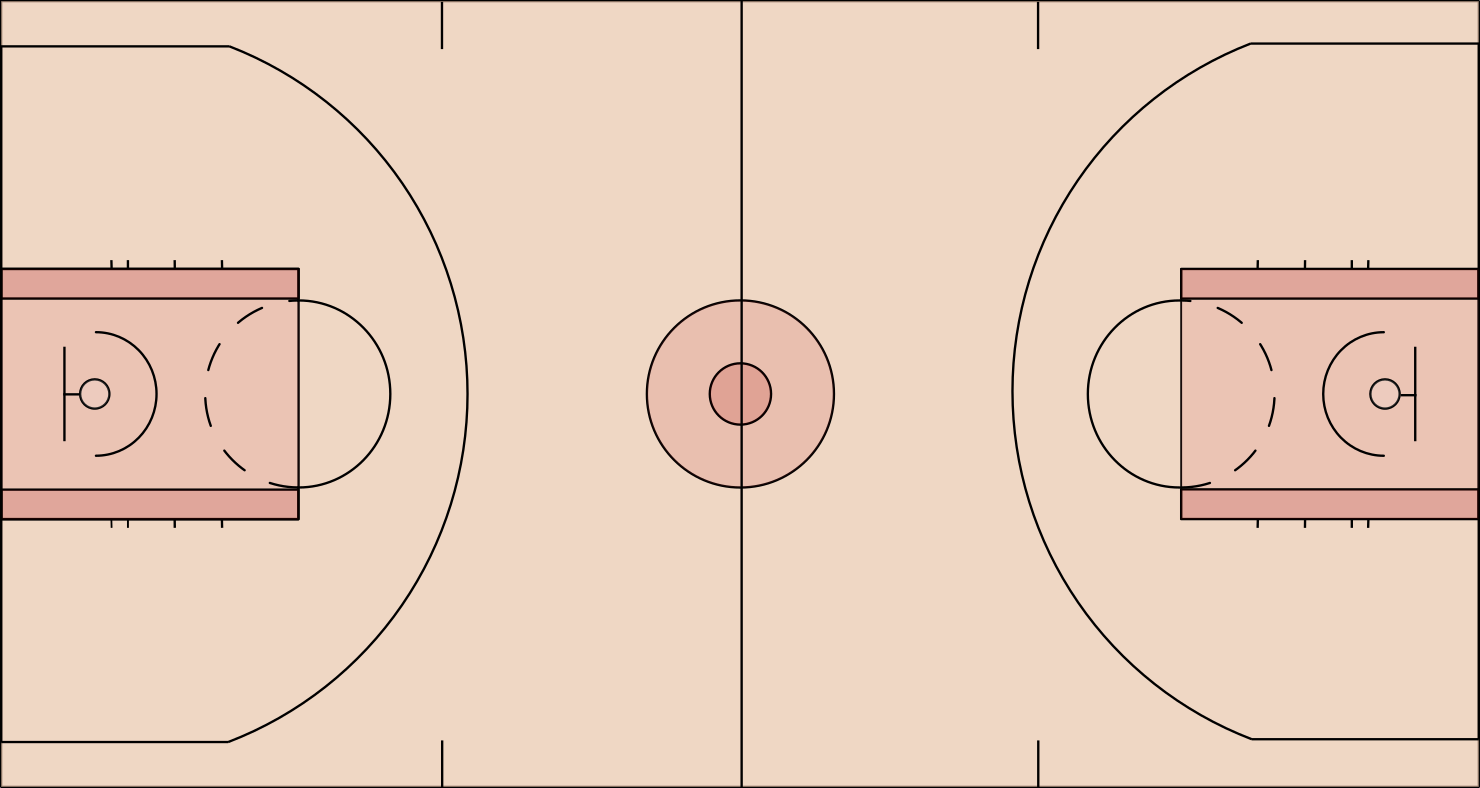
\includegraphics[width=\textwidth]{contents/nba_court.png}
    \caption{Diagram of a typical NBA basketball court.}
    \label{fig:nba_court}
\end{figure}

\paragraph {overview:}
\label{sect:original_nba}

To facilitate the development and validation of these models, this study utilizes a dataset sourced from the ``NBA-Player-Movements'' repository by Linou et al. \cite{linouk}. The dataset contains 636 games from the 2015/16 season. Each game is stored in a compressed ``.7z'' format, which can be extracted using tools such as 7zip. Once extracted, the data is presented in a ``.json'' format, which was further processed using Python to prepare it for analysis. Upon reading the JSON file into a pandas DataFrame, the data is structured with three primary columns: \textbf{``gameid''}, \textbf{``gamedate''}, and \textbf{``events''}. The \textbf{``gameid''} and \textbf{``gamedate''} columns contain the unique identifier for each game and the corresponding date, respectively. These values remain constant for each row (event) within a single game. The \textbf{``events''} column contains detailed information about each individual event, represented as a dictionary. The keys of this dictionary are \textbf{``eventId''}, \textbf{``visitor''}, \textbf{``home''}, and \textbf{``moments''}. Information regarding the \textbf{``visitor''} and \textbf{``home''} keys, which provide details about the teams involved, is discussed in Section \ref{sect:teams}. Details about the \textbf{``moments''} key, which contains information on specific moments within events, will be elaborated on in Section \ref{sect:moments}. Figure \ref{fig:data-structure} provides a graphical representation of the dataset structure, illustrating the organization of the data columns and the relationships between different elements, including the main file structure, team details, and moment details.

\paragraph {Home and Visitor Team:}
\label{sect:teams}

In the dataset, information about both the home and visitor teams is provided under the \textbf{``home''} and \textbf{``visitor''} keys, respectively. Each team is represented as a dictionary that contains several important details. Specifically, the dictionary includes the team's \textbf{``name''}, which is its official designation, the \textbf{``teamid''}, a unique identifier used to distinguish the team from others, and the \textbf{``abbreviation''}, which is a short code representing the team’s name for convenience.

Within each team dictionary, there is a \textbf{``players''} key that points to a list of dictionaries. Each dictionary in this list represents an individual player on the team. For each player, the dictionary includes the \textbf{``lastname''} and \textbf{``firstname''}, which together identify the player. It also includes the \textbf{``playerid''}, a unique identifier for the player, and the \textbf{``jersey''} number, which is unique within the team and indicates the player's number. Lastly, the \textbf{``position''} describes the player’s role on the team, such as forward, center, or guard. Figure \ref{fig:data-structure} shows the structure graphically. 

\paragraph {Moments:}
\label{sect:moments}

The \textbf{``moments''} key in the dataset provides detailed information about specific events within the game. Each entry under this key is a list of \textbf{``moment''}s, where each \textbf{``moment''} contains several pieces of information. These details include the \textbf{``quarter''}, which indicates the quarter number during which the moment occurred, and the \textbf{``moment\_id''}, representing the absolute timestamp of the moment in UNIX format. Additionally, \textbf{``game\_clock''} and \textbf{``shot\_clock''} provide further temporal information, measured in seconds. The \textbf{``None''} field typically remains empty and does not contain any data. The \textbf{``objects''} key within each moment lists the details of all players on the field and the ball, usually totaling 11 entries: 5 players from each team and the ball. For each entry, the data includes \textbf{``teamid''} and \textbf{``playerid''}, which are consistent across all moments. Additionally, \textbf{``x\_pos''} and \textbf{``y\_pos''} provide the positional information of each player in feet, with the origin defined as the lower left corner of the field. The \textbf{``ball\_radius''} is relevant only for the ball, providing its radius, which indirectly gives information about the ball's height or z-axis position. For a visual representation of the structure of these moment details, please refer to Figure \ref{fig:data-structure}.

\begin{figure}[t]
\centering
\includesvg[width=\textwidth]{contents/data-structure.svg}
\caption{Graphical representation of the dataset structure, including the main file (left) and details about the home and vistor teams (center), and moments~(right).}
\label{fig:data-structure}
\end{figure}


\paragraph {Data Preparation and Transformation:}
\label{sect:data-prep}

To create a usable dataset, several preparation steps were undertaken. The complex nested structure described earlier was simplified into a more manageable two-dimensional DataFrame. Each moment was converted into a row, with all relevant information contained within these rows. While this transformation increased disk usage due to the replication of data, such as game dates and game IDs, which were previously represented only once per match, the trade-off was justified by the improved accessibility and ease of use gained through flattening the structure.

Each moment contains data for 11 objects—comprising 5 players from each team and the ball—each with distinct attributes, specifically position and velocity. To streamline the dataset, unnecessary fields were removed, including \textbf{``firstname''}, \textbf{``lastname''}, \textbf{``jersey''}, \textbf{``teamname''}, \textbf{``gamedate''}, and irrelevant fields such as the \textbf{``None''} column. This decision was based on the focus of the task, which required generalizable models rather than identification of individual players or teams. By retaining only the essential data, such as the game name in the filename and removing these extraneous columns, disk space usage was reduced by precisely \(62.30\%\).

The resulting dataset contains, for each moment, the positions (\textbf{x\_pos}, \textbf{y\_pos}) and velocities (\textbf{vx}, \textbf{vy}) of all 10 players and the ball. These positions are specified in feet, with the origin defined at the lower left corner of the court. The velocity data is derived from the positional changes over time and provides crucial information for dynamic~analysis.

The original dataset was recorded primarily in 0.04-second intervals, equating to a sampling rate of 25Hz. However, due to occasional missing data points, some time spans were incomplete. To ensure consistency and maintain the temporal resolution, these gaps were filled using interpolation. Missing values were interpolated to preserve the integrity of the time series data, enabling a seamless analysis of player and ball movements.

To further enhance consistency, the rows were sorted by ascending event numbers and then by \textbf{"moment\_id"} within each event. Additionally, events with fewer than 8 seconds of data (or fewer than 200 \textbf{"moments"}) were excluded to maintain consistency across the dataset and reduce the risk of bias from shorter events, which are typically not useful for many models. After cleaning, the dataset shrank by 36.44\%, resulting in approximately 163,000 remaining events.

The overall reduction in data size, considering both row and column cleaning, was calculated as 
\[
z = 1 - (1 - x)(1 - y) = 1 - (1 - 0.623)(1 - 0.3644) \approx 0.76 
\]
This indicates that more than three-quarters of the original data was ultimately removed during preprocessing. The final dataset is a single two-dimensional DataFrame consisting solely of the unique \textbf{event\_id}, unique \textbf{moment\_id}, and the positions and velocities of all players and the ball.

To prepare the data for model training, the dataset was split into training and validation sets using a 95-5 ratio. All games except the specific game, \textbf{TOR@LAL}, where \textbf{TOR} is the visiting team and \textbf{LAL} is the home team, were included in these sets. This particular game, \textbf{TOR@LAL}, was set aside as the testing dataset. The training and validation sets consist of 6,365 events (2,131,840 moments), with 6,047 events used for training and 318 events for validation. The separate testing dataset comprises 153 events (57,504 moments). This split allows an examination of how well the model generalizes from one team to another, providing insights into its performance and adaptability in various contexts.

\textbf{Velocity Calculation for Each Time Step:}  
To compute the velocity from the positional data provided in the \textbf{``x\_pos''} and \textbf{``y\_pos''} fields at each moment, three differentiation methods are employed, depending on the time step. Special cases are required for the first and last time steps due to the lack of neighboring data points at these boundaries. The calculated velocities are saved as \textbf{``x\_vel''} and \textbf{``y\_vel''} alongside with the index of the player:

\begin{itemize}
    \item \textbf{First Time Step (Forward Differentiation):} For the first time step, velocity is approximated using forward differentiation:
    \[
    v(t_0) = \frac{x(t_1) - x(t_0)}{\Delta t}
    \]
This method is applied because there is no available preceding time step for backward differentiation, necessitating the use of a one-sided differentiation approach.

    \item \textbf{Intermediate Time Steps (Central Differentiation):} For all intermediate time steps, velocity is calculated using central~differentiation:
    \[
    v(t_i) = \frac{x(t_{i+1}) - x(t_{i-1})}{2 \Delta t}
    \]
    This method provides a more accurate approximation of velocity at each intermediate time step \( t_i \) by utilizing both neighboring~points.

    \item \textbf{Last Time Step (Backward Differentiation):} At the final time step, velocity is estimated using backward~differentiation:
    \[
    v(t_n) = \frac{x(t_n) - x(t_{n-1})}{\Delta t}
    \]
    This approach is employed because there is a lack of subsequent data points required for forward differentiation, resulting in the necessity of one-sided differentiation.
\end{itemize}


\subsection{Soccer}
\label{sect:SOC}
Soccer, similar to basketball, is a dynamic and fast-paced sport where two teams compete to control the ball and score goals. Both sports emphasize teamwork, strategy, and quick decision-making, making them useful for testing similar predictive models. However, a key difference lies in the playing field. Unlike the strictly regulated NBA court, which measures approximately 28.65 meters in length and 15.24 meters in width, soccer fields are not uniformly sized across all datasets or competitions. The size of a soccer field can vary significantly, typically ranging between 100-110 meters in length and 64-75 meters in width. This variability in field dimensions can introduce additional complexity when processing soccer data for comparison with basketball data.

To address this, it is crucial to normalize the soccer dataset into the same format as the NBA dataset \ref{sect:NBA} for consistency in analysis and accurate comparison between the two sports. The soccer court dimensions used in this dataset are illustrated in Figure \ref{fig:soccer_court}, which provides a visual representation of the standard field layout and dimensions.

\begin{figure}[t]
    \centering
    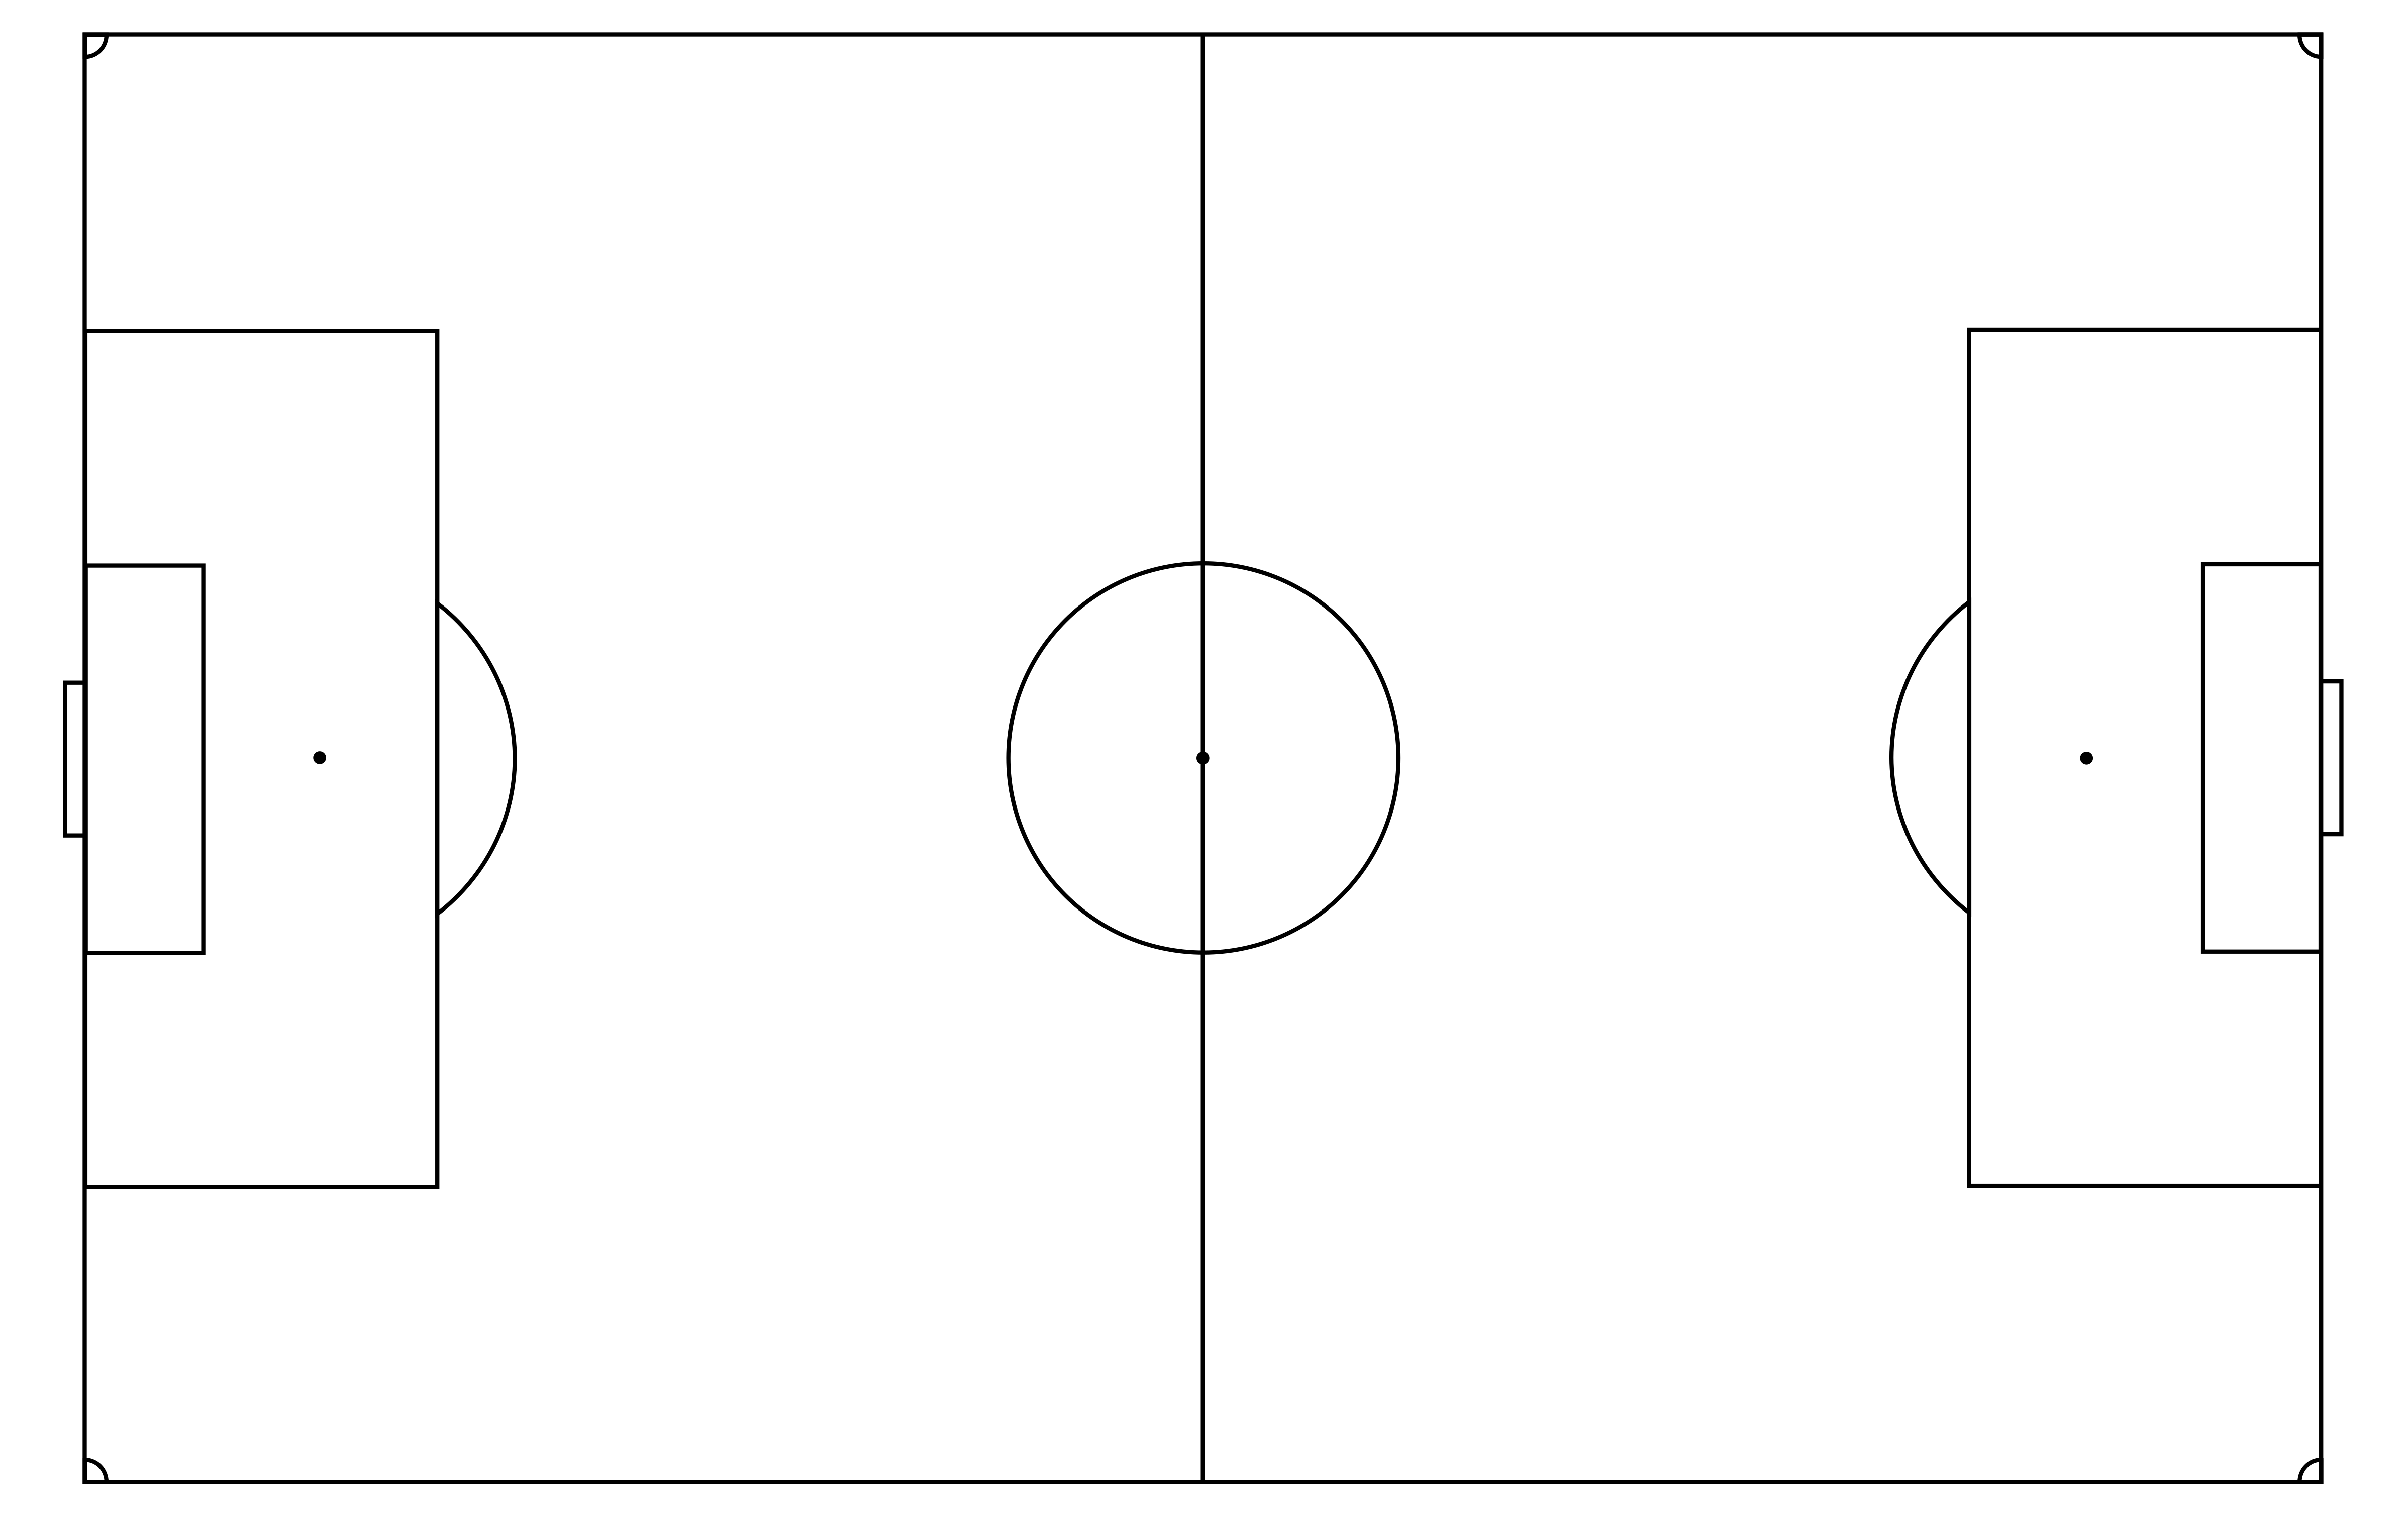
\includegraphics[width=\textwidth]{contents/drawing_rg.png}
    \caption{Diagram of a typical DFL soccer field.}
    \label{fig:soccer_court}
\end{figure}



\paragraph {overview:}
\label{soc:details}
The Soccer dataset consists of 316 games from the Deutsche Fu{\ss}ball Liga (DFL) for the 2014/15 and 2015/16 seasons and was provided by the Fraunhofer Institute for Integrated Circuits IIS. Unlike the original NBA files, the Soccer dataset is flat and straightforward. It is organized into two separate two-dimensional datasets: one for the ball \ref{sect:ball} and one for the players \ref{sect:players}. In this dataset, information about players, teams, and games is replaced with encrypted text to ensure privacy and anonymity.

\paragraph {Ball:}
\label{sect:ball}
The dataset also includes detailed information about the ball at every moment during the game. The relevant fields are \textbf{BallStatus}, \textbf{M}, \textbf{N}, \textbf{Period}, \textbf{S}, \textbf{T}, \textbf{TeamBallPossession}, \textbf{X}, and \textbf{Y}. Specifically, \textbf{BallStatus} indicates the current status of the ball, such as whether it is in play or not. The \textbf{N} column represents the moment identifier, which shows the sequence of recorded moments, and \textbf{M} is the event number within the game. The \textbf{Period} field denotes the current period of the game (e.g., 1st quarter, 2nd quarter), while \textbf{S} provides a timestamp marking the specific moment in seconds since the start of the event. The \textbf{T} field shows the absolute time in milliseconds since the start of the game. The \textbf{TeamBallPossession} indicates which team has possession of the ball at a given moment, and \textbf{X} and \textbf{Y} represent the x and y coordinates of the ball’s position on the court, respectively. Each row in the dataset corresponds to a particular moment, capturing the ball's position and status during that time. In snippet \ref{fig:ball-dataset} , the \textbf{BallStatus} field shows whether the ball is in play. The \textbf{M} column indicates these are sequential moments within the same period of the game. The \textbf{S} field represents the time in seconds within the current event, while \textbf{T} provides the absolute time in milliseconds since the game's start.

The \textbf{TeamBallPossession} field reveals which team had possession of the ball, and the \textbf{X} and \textbf{Y} fields track the ball's movement on the court.

\begin{figure}[H]
    \centering
    \begin{BVerbatim}
    BallStatus,M,N,Period,S,T,TeamBallPossession,X,Y
0,1,10000,1,6.38,1418481028680,DFL-CLU-00000G, 9.85,37.12
1,1,10001,1,6.35,1418481028720,DFL-CLU-00000G, 9.82,37.06
1,1,10002,1,6.36,1418481028760,DFL-CLU-00000G, 9.80,36.99
1,1,10003,1,6.38,1418481028800,DFL-CLU-00000G,10.33,37.37
1,1,10004,1,1.96,1418481028840,DFL-CLU-00000G,10.02,37.29
1,1,10005,1,2.68,1418481028880,DFL-CLU-00000G,10.09,37.44
    \end{BVerbatim}
    \caption{snippet of the Ball dataset for Soccer}
    \label{fig:ball-dataset}
\end{figure}



\paragraph {Players:}
\label{sect:players}

The dataset includes detailed information for each player, captured at every moment within the game. The relevant fields in the dataset are \textbf{M}, \textbf{N}, \textbf{Period}, \textbf{PersonId}, \textbf{PlayingPosition}, \textbf{S}, \textbf{T}, \textbf{TeamId}, \textbf{X}, and \textbf{Y}, which represent crucial attributes of each player. Specifically, \textbf{N} is the moment identifier indicating the sequence of recorded moments, \textbf{M} is the event number within the game, and \textbf{Period} refers to the current period of the game (e.g., 1st quarter, 2nd quarter). The \textbf{PersonId} is a unique identifier for each player, anonymized in this dataset, and \textbf{PlayingPosition} denotes the player's position on the court (e.g., guard, forward). The \textbf{S} field provides a timestamp marking the specific moment in seconds since the start of the event, while \textbf{T} represents the absolute time in milliseconds since the start of the game. The \textbf{TeamId} uniquely identifies the team to which the player belongs, and the \textbf{X} and \textbf{Y} fields capture the x and y coordinates of the player's position on the court. The code snipped \ref{fig:player-dataset} illustrates an example.


\begin{figure}[H]
    \centering
    \begin{BVerbatim}
           M,N,Period,PersonId,PlayingPosition,S,T,TeamId,X,Y
1,10000,1,DFL-OBJ-00001T,IVL,0.00,1418412626360,DFL-CLU-00000F,-26.36, 9.95
1,10001,1,DFL-OBJ-00001T,IVL,2.04,1418412626400,DFL-CLU-00000F,-26.36, 9.96
1,10002,1,DFL-OBJ-00001T,IVL,2.08,1418412626440,DFL-CLU-00000F,-26.36, 9.97
1,10003,1,DFL-OBJ-00001T,IVL,2.05,1418412626480,DFL-CLU-00000F,-26.36, 9.98
1,10004,1,DFL-OBJ-00001T,IVL,1.90,1418412626520,DFL-CLU-00000F,-26.36,10.00
1,10005,1,DFL-OBJ-00001T,IVL,1.90,1418412626560,DFL-CLU-00000F,-26.36,10.01
    \end{BVerbatim}
    \caption{snippet of the Player dataset for Soccer}
    \label{fig:player-dataset}
\end{figure}


\paragraph {Data Preparation and Transformation:}
\label{sect:data-prep-soccer}

For the soccer dataset, a similar preparation process was employed. The data was recorded at 25Hz (0.04-second intervals) and was mostly consistent, with interpolation being used to fill in any missing or erroneous data points. The entire dataset was split into training and validation sets using a 95-5 ratio, while the game \textbf{0002ZV} was used exclusively as the testing dataset. The training and validation sets consist of 2,786 trajectories (4,194,182 moments), with 2,646 trajectories used for training and 140 for validation. The testing dataset contains 88 trajectories (130,711 moments). The dataset was structured to integrate player and ball information into a single, unified format. Each row in the dataset contained all relevant attributes for a specific moment, including positions (\textbf{x\_pos}, \textbf{y\_pos}) and velocities (\textbf{vx}, \textbf{vy}) for both players and the ball. To ensure comprehensive analysis, all these attributes were combined into single rows, allowing for a detailed examination of player and ball dynamics throughout the game. In the process of cleaning the dataset, certain fields were deemed unnecessary for the current study. Specifically, for the ball data, the following keys were removed: \textbf{BallStatus}, \textbf{Period}, \textbf{S}, and \textbf{TeamBallPossession}. For player data, the keys \textbf{Period}, \textbf{PersonID}, \textbf{Playing Position}, \textbf{S}, and \textbf{TeamID} were also excluded. These fields did not contribute to the core analysis and thus were removed to streamline the dataset. To enhance the dataset's utility, velocity information was introduced. Velocity calculations for each time step followed the same differentiation methods as described in the NBA dataset preparation Section (see Section \ref{sect:data-prep}), using forward, central, and backward differentiation techniques depending on the position in the time series.
The final dataset is a two-dimensional DataFrame that integrates the positions and velocities of all players and the ball. All rows contained more than 8 seconds of data, meaning no data was excluded based on duration. However, it was essential to verify this criterion to ensure consistency. This dataset is designed to support detailed analysis and modeling, enabling insights into player behavior, game strategies, and overall dynamics. The structured approach to data preparation ensures that the dataset is both comprehensive and reliable for training and evaluating models.



\section{Experiments}
\label{sec:experiments}

This Section describes the experimental setup designed to address key research questions regarding model performance. Each experiment is tailored to explore a specific aspect of the problem, providing insights that directly answer the research questions posed in this study. The Results of the experiments are shown in Chapter \ref{chapt:results}.

\subsection{E1: Attention-Based versus Baseline Models}
\label{exp:e1}
This experiment addresses Question Q1: \textbf{How do attention-based models compare to other models in general?} We evaluate the performance of attention-based models, particularly the Transformer, against baseline models such as 1LL, 2LL, LSTM, and LMU. All models are trained and tested on the NBA and DFL datasets using the full input context, with \texttt{features\_in} = 4 (velocity and positional information) and the full \SI{2.0}{\second} historical context. The number of objects is \texttt{num\_objects} = 25 for the NBA (2 × 11 players + 1 ball + 2 baskets) and \texttt{num\_objects} = 13 for soccer (2 × 5 players + 1 ball + 2 goals). All models in this Section are multivariate, handling all variables together. The aim is to compare forecasting accuracy, energy consumption, and training time to assess the effectiveness of attention mechanisms in human motion forecasting.

\subsection{E2: Evaluating Impact of Input Exclusions}
\label{exp:e2}
This experiment addresses Question Q2: \textbf{How does model performance vary when positional or velocity data is excluded?} For each model, we assess a version excluding either positional or velocity data, resulting in \texttt{features\_in} = 2 during training and testing. By analyzing the changes in forecasting accuracy and robustness, we aim to determine the impact of each data type on model performance. This investigation will provide insights into the trade-offs between computational efficiency and predictive accuracy, thereby informing optimal input strategies for human motion forecasting.


\subsection{E3: Robustness to Reduced Historical Information}
\label{exp:e3}
This experiment addresses Question Q3: \textbf{How robust is each model to reduced historical information?} We evaluate all models using the full context of \texttt{features\_in} = 4 but with shortened historical lengths. The historical input is reduced from the original \SI{2}{\second} (50 frames) to \SI{1}{\second} (25 frames), \SI{0.4}{\second} (10 frames), and \SI{0.04}{\second} (1 frame) on the \SI{25}{\hertz} dataset. By examining how each model's performance changes with these varying time intervals, we aim to assess their adaptability and accuracy in forecasting human motion with reduced historical data. This analysis will identify which models exhibit greater resilience and reliability when extensive historical context is unavailable.

\subsection{E4: Comparing Univariate and Multivariate Predictors}
\label{exp:e4}
This experiment addresses Question Q4: \textbf{How does a multivariate predictor compare to multiple univariate predictors in terms of forecasting accuracy?} We use the full context with \texttt{features\_in} = 4 and the complete \SI{2}{\second} historical length. In this experiment, we split the x-axis and y-axis into two separate univariate models for each architecture, with one model processing the x-axis data and the other processing the y-axis data. The linear models 1LL and 2LL are not investigated in this case due to a lack of interest. This comparison aims to determine whether the original multivariate models, capable of capturing interactions between axes, outperform their univariate counterparts or if independently processing each axis yields better forecasting accuracy.


\subsection{E5: Generalization Across Different Teams}
\label{exp:e5}
This experiment tackles Question Q5: \textbf{How do the models generalize to other teams?} We evaluate the generalization capabilities of the models using the full input context and historical length. For the NBA dataset, the models are trained solely on the Los Angeles Lakers, with the Toronto Raptors serving as the unseen team for testing. In the soccer dataset, the models are trained only on the anonymized team 00000F, with the anonymized team 0002ZV as the unseen team. This approach allows us to assess how well each model adapts to different team dynamics and behaviors. Understanding the extent to which these models can generalize is crucial for their application in real-world scenarios, where variability in team performance is common.


\subsection{E6: Transfer Learning with Pre-trained Models}
\label{exp:e6}
This experiment addresses Question Q6: \textbf{How does transfer learning impact model performance when trained on one domain and fine-tuned on another?} This analysis is conducted with a reduced input context of one object, specifically including the ball and the basketball/goal information, resulting in \texttt{num\_objects} = 4 per timestep. We will investigate the efficacy of transfer learning by initially training our models on a dataset from one team or sport and then fine-tuning them on a different team or sport. This approach helps evaluate how well the pretrained models adapt to the new context and whether this transfer leads to improved performance. Understanding the benefits of transfer learning is crucial for enhancing model robustness and applicability in diverse team-based sports environments.

\subsection{E7: Evaluating Player Performance in Isolation}
\label{exp:e7}
This experiment addresses Question Q7: \textbf{How does each model perform when predicting the movement of a single target player using only that player's data, excluding the social-interaction context?} In this experiment, we utilize the full input context and length, but the number of players has been reduced to one player per game, resulting in \texttt{num\_objects} = 4 (1 player + 1 ball + 2 baskets for NBA, and 1 player + 1 ball + 2 goals for soccer). We train each model using only the data from the target player, effectively removing the influence of other players' movements. We then evaluate the models' forecasting accuracy based on this limited input. By analyzing the results, we aim to understand the impact of excluding social-interaction information on each model's performance in predicting individual player dynamics.



\section{Model Configurations}
\label{sec:model_configurations}

This Section provides an overview of the configurations used for training each of the six models: 1LL, 2LL, LSTM, LMU, Transformer, and BitNet. Details about the architectures of each model can be found in Section \ref{sec:main_proc}. Here, we list the main hyperparameters used for training, such as hidden size, learning rate, and other relevant configurations for each model. All models were trained using the AdamW optimizer \cite{adamw}, which is known for its effective handling of sparse gradients and improved convergence properties. The learning rate was kept consistent across all models, set to \texttt{learning\_rate} of $0.001$.

\begin{itemize}
    \item \textbf{One Layer Linear Model (1LL):} 
    No additional configurations are provided for the 1LL model (see Section \ref{sec:1ll-details}).
    
    \item \textbf{Two Layer Linear Model (2LL):} 
    The 2LL model (see Section \ref{sec:2ll-details}) has a \texttt{hidden\_size} of $1024$ and a \texttt{dropout\_rate} of $0.1$.
    
    \item \textbf{Long Short-Term Memory Model (LSTM):} 
    The LSTM model (see Section \ref{sec:lstm-details}) has a \texttt{hidden\_size} of $256$ and a \texttt{dropout\_rate} of $0.1$.
    
    \item \textbf{Legendre Memory Unit Model (LMU):} 
    The LMU model (see Section \ref{sec:lmu-details}) has a \texttt{hidden\_size} of $256$, a \texttt{memory\_size} of $256$, and a \texttt{dropout\_rate} of $0.1$. Additionally, the parameters \texttt{learn\_a} and \texttt{learn\_b} are set to true.
    
    \item \textbf{Transformer Model:} 
    The Transformer model (see Section \ref{sec:transformer-details}) employs a convolutional layer as the positional encoder, which has a \texttt{kernel\_size} of $3$, a \texttt{stride} of $1$, and \texttt{padding} of $1$. The Transformer has a \texttt{hidden\_size} of $256$, \texttt{n\_blocks} of $6$, \texttt{n\_heads} of $8$, \texttt{ffn\_hiddens} of $1024$, and a \texttt{dropout\_rate} of $0.1$. Additionally, the Transformer introduces a learning rate warm-up, as described in Section \ref{sec:scheduler}, with 1000 warm-up steps.
    
    \item \textbf{BitNet Model:} 
    Similar to the Transformer model, the BitNet model (see Section \ref{sec:bitnet-details}) employs a convolutional layer as the positional encoder, with a \texttt{kernel\_size} of $3$, a \texttt{stride} of $1$, and \texttt{padding} of $1$. The BitNet has a \texttt{hidden\_size} of $256$, \texttt{n\_blocks} of $6$, \texttt{n\_heads} of $8$, \texttt{ffn\_hiddens} of $1024$, and a \texttt{dropout\_rate} of $0.1$. The BitNet does not include a warm-up scheduler.
\end{itemize}


\section{Training Details}
\label{sec:training_details}

The training details for the main models on the \gls{nba} and \gls{dfl} datasets are presented below. All models were trained with a patience of 20 epochs, and energy consumption was measured using Courty et al.'s CodeCarbon \cite{codecarbon}, an estimation tool for energy usage during training. For both \gls{nba} and \gls{dfl} datasets, the same hyperparameters were utilized, since our aim is to provide a generalizable model, which doesn't have to be configured for each sport separately.

Due to the high memory requirements of attention-based models such as the Transformer and BitNet, a batch size of 16 was used to prevent out-of-memory situations during training. In contrast, other models with lower memory requirements were able to be trained with a larger batch size of 64.

The detailed training metrics for each model are summarized in Table \ref{training_details_nba} for the NBA dataset and Table \ref{training_details_soccer} for the Soccer dataset. These tables provide insights into the following metrics: Parameters in Millions, Model Size in Megabytes (MB), batch size, number of Epochs, Training Loss measured as Mean Squared Error (MSE) in meters, Energy Consumption in milliwatt-hours ($\si{\milli\watt\hour}$), Energy per Epoch (En. per ep.) in milliwatt-hours ($\si{\milli\watt\hour}$), and Training Time (Tr. time) in the format (hh:mm:ss).




\begin{table}[b]
    \centering
    \caption[Table of Training details for NBA Dataset]{This table provides detailed training details of every model for the nba dataset.}
    \begin{tabular}{l||c|c|c|c|c|c}
        \label{training_details_nba}
        \textbf{Metric} & \textbf{1LL} & \textbf{2LL} & \textbf{LSTM} & \textbf{LMU} & \textbf{Trafo} & \textbf{BitNet} \\ \hline \hline
        Params (M) & 0.520 & 2.9 & 0.895 & 0.303 & 4.9 & 4.9 \\ \hline 
        Model Size (MB) & 2.081 & 11.474 & 3.581 & 1.213 & 19.430 & 19.541 \\ \hline 
        batch\_size & 64 & 64 & 64 & 64 & 16 & 16 \\ \hline 
        
        Epochs & 46 & 34 & 82 & 97 & 46 & 79 \\ \hline 
        Train Loss (\si{\meter})& 2.44 & 1.86 & 1.66 & 1.66 & 1.66 & 1.77 \\ \hline
        Energy (\si{\milli\watt\hour}) & 30.05 & 29.04 & 33.53 & 141.85 & 206.02 & 324.54 \\ \hline
        En. per ep. (\si{\milli\watt\hour}) & 0.65 & 0.85 & 0.41 & 1.46 & 4.48 & 4.11 \\ \hline
        Tr. Time (hh:mm:ss) & 00:01:34 & 00:01:28 & 00:08:59 & 02:09:21 & 00:44:15 & 02:46:55 \\ 
    \end{tabular}
\end{table}

\begin{table}[b]
    \centering
    \caption[Table of Training details for Soccer Dataset]{This table provides detailed training details of every model for the Soccer dataset.}    
    \begin{tabular}{l||c|c|c|c|c|c}
    \label{training_details_soccer}
    \textbf{Metric} & \textbf{1LL} & \textbf{2LL} & \textbf{LSTM} & \textbf{LMU} & \textbf{Trafo} & \textbf{BitNet} \\ \hline \hline
    Params (M) & 1.0 & 5.3 & 0.944 & 0.315 & 4.9 & 4.9 \\ \hline 
    Model Size (MB) & 4.001 & 21.304 & 3.777 & 1.263 & 19.578 & 19.688 \\ \hline 
    batch\_size & 64 & 64 & 64 & 64 & 16 & 16 \\ \hline 
    
    Epochs & 70 & 121 & 70 & 129 & 53 & 132 \\ \hline 
    Train Loss (\si{\meter})& 3.37 & 1.82 & 1.08 & 1.01 & 1.08 & 1.27 \\ \hline
    Energy (\si{\milli\watt\hour}) & 19.07 & 20.77 & 27.35 & 131.21 & 107.94 & 192.50 \\ \hline
    En. per ep. (\si{\milli\watt\hour}) & 0.30 & 0.17 & 0.39 & 1.02 & 2.04 & 1.46 \\ \hline
    Tr. Time (hh:mm:ss) & 00:02:03 & 00:04:02 & 00:04:32 & 01:20:06 & 00:25:12 & 02:13:51 \\ 
    \end{tabular}
\end{table}


\chapter{Results}
\label{chapt:results}
This Chapter introduces the metrics needed to evaluate and benchmark model performance, as detailed in Section \ref{sec:metrics}. Subsequently, Section \ref{sec:eval} presents a thorough evaluation of the experiments conducted in \ref{sec:experiments}, including model performance and comparative~analysis.


\section{Metrics}
\label{sec:metrics}
This section outlines the metrics used for evaluating trajectory prediction models. These include \gls{mse} and \gls{mae} for fundamental accuracy, \gls{fde} and \gls{ade} for positional accuracy, \gls{nlade} for non-linear trajectory segments, and \gls{fae} and \gls{aae} for directional accuracy. Details for each metric are provided in Sections \ref{eq:mse} to \ref{eq:aae}.

\subsection{Mean Squared Error}
\label{eq:mse}
\gls{mse} quantifies the average squared difference between predicted and true values. It is defined as:
\begin{align}
\setequationentry{Mean Squared Error}
    \text{MSE} &= \frac{1}{n \cdot m} \sum_{i=1}^n \sum_{j=1}^m \left( \hat{y}_{i,j} - y_{i,j} \right)^2
\end{align}

where \(\hat{y}_{i,j}\) and \(y_{i,j}\) are the predicted and actual values, respectively, for the \(i\)-th sample and \(j\)-th feature, \(n\) is the number of samples, and \(m\) is the number of features. This meassurement is also used to train the models.

\subsection{Mean Absolute Error}
\label{eq:mae}
\gls{mae} measures the average magnitude of the errors in a set of predictions, without considering their direction:
\begin{align}
\setequationentry{Mean Absolute Error}
    \text{MAE} &= \frac{1}{n \cdot m} \sum_{i=1}^n \sum_{j=1}^m \left| \hat{y}_{i,j} - y_{i,j} \right|
\end{align}

\subsection{Final Displacement Error}
\label{eq:FDE}
\gls{fde} calculates the Euclidean distance between the predicted final position and the true final position at time \(T_{\text{pred}}\):
\begin{align}
\setequationentry{Final Displacement Error}
    \text{FDE} &= \frac{1}{n}\sum_{i=1}^n \left( (\hat{y}_{T_{pred},i} - y_{T_{pred},i})^2 \right)
\end{align}
This metric is discussed in detail by Xu et al. \cite{xu2018collision}.

\subsection{Average Displacement Error}
\label{eq:ADE}
\gls{ade} measures the mean squared error over all predicted points in the trajectory:
\begin{align}
\setequationentry{Average Displacement Error}
    \text{ADE} &= \frac{\sum_{i=1}^n \sum_{t=T_{\text{obs}}+1}^{T_{\text{pred}}} \left( (\hat{y}_{t,i} - y_{t,i})^2 \right)}{n \cdot (T_{\text{pred}} - (T_{\text{obs}} + 1))}
\end{align}
This metric is also discussed by Xu et al. \cite{xu2018collision}.

\subsection{Average Non-Linear Displacement Error}
\label{eq:nl-ade}
\gls{nlade} focuses on the MSE in non-linear regions of a trajectory, calculated as:
\begin{align}
\setequationentry{Non-Linear Average Displacement Error}
    \text{NL-ADE} &= \frac{\sum_{i=1}^n \sum_{t=T_{\text{obs}}+1}^{T_{\text{pred}}} I_{t,i}  (\hat{y}_{t,i} - y_{t,i})^2}{\sum_{i=1}^n \sum_{t=T_{\text{obs}}+1}^{T_{\text{pred}}} I_{t,i}}
\end{align}

where \(I_{t,i}\) is an indicator function that equals 1 if the trajectory has a non-zero curvature at time \(t\) and 0 otherwise \cite{xu2018collision}. Human movements are dynamic and continuously changing. To make \gls{nlade} useful, it is necessary to introduce a threshold, for example, \(\delta v = 0.5 \text{m/s}\). Trajectories with curvature below this threshold would be considered not non-linear enough.

\subsection*{Angular Error}
\label{eq:angular error}
\gls{ae} quantifies the discrepancy between the predicted and true velocity vectors. It can be measured using the cosine similarity, defined as:
\begin{align}
\setequationentry{Cosine Similarity}
    \cos \theta_{t,i} &= \frac{\mathbf{v}_{t,i} \cdot \hat{\mathbf{v}}_{t,i}}{\|\mathbf{v}_{t,i}\| \|\hat{\mathbf{v}}_{t,i}\|} \\
\setequationentry{Angular Error}
\label{angular_error}
    \theta_{t,i} &= \text{arccos} \left( \frac{\mathbf{v}_{t,i} \cdot \hat{\mathbf{v}}_{t,i}}{\|\mathbf{v}_{t,i}\| \|\hat{\mathbf{v}}_{t,i}\|} \right)
\end{align}

where \(\mathbf{v}_{t,i}\) and \(\hat{\mathbf{v}}_{t,i}\) are the true and predicted velocity vectors, respectively, at time \(t\). For numerical stability, a small \(\epsilon\) is added to the denominator.


\subsection{Final Angular Error}
\label{eq:fae}
\gls{fae} measures the angular discrepancy at the final time step \(T_{\text{pred}}\). It is computed as:
\begin{align}
\setequationentry{Final Angular Error}
    \text{FAE} &= \frac{1}{n} \sum_{i=1}^n \left| \theta_{T_{\text{pred}},i} - \theta_{T_{\text{pred}},i}^\text{true} \right| \times \frac{180}{\pi}
\end{align}

where \(\theta_{T_{\text{pred}},i}\) is the \gls{ae} calculated at \(T_{\text{pred}}\) as defined in \eqref{angular_error}.

\subsection{Average Angular Error}
\label{eq:aae}
\gls{aae} computes the mean angular difference between predicted and true velocity vectors over all time steps. It is defined as:
\begin{align}
\setequationentry{Average Angular Error}
    \text{AAE} &= \frac{1}{n \cdot (T_{\text{pred}} - T_{\text{obs}})} \sum_{i=1}^n \sum_{t=T_{\text{obs}}+1}^{T_{\text{pred}}} \theta_{t,i} \times \frac{180}{\pi}
\end{align}

where \(\theta_{t,i}\) is the \gls{ae} calculated for trajectory \(i\) at time \(t\) as defined in \eqref{angular_error}.

These metrics offer a comprehensive assessment of trajectory prediction performance, capturing various dimensions of accuracy and error.
\FloatBarrier

\section{Experiment Evaluation}
\label{sec:eval}
This Chapter introduces the metrics needed to evaluate and benchmark model performance, as detailed in Section \ref{sec:metrics}. Subsequently, Section \ref{sec:eval} presents a thorough evaluation of the experiments conducted in \ref{sec:experiments}, including model performance and comparative~analysis.

\subsection{E1: Attention-Based versus Baseline Models}

This Section introduces the results of Experiment 1 \ref{exp:e1} which incestigates the question \textbf{Q1: How do attention-based models compare to other models in general?}.
\label{exp:init}
\begin{figure}[t]
    \centering
    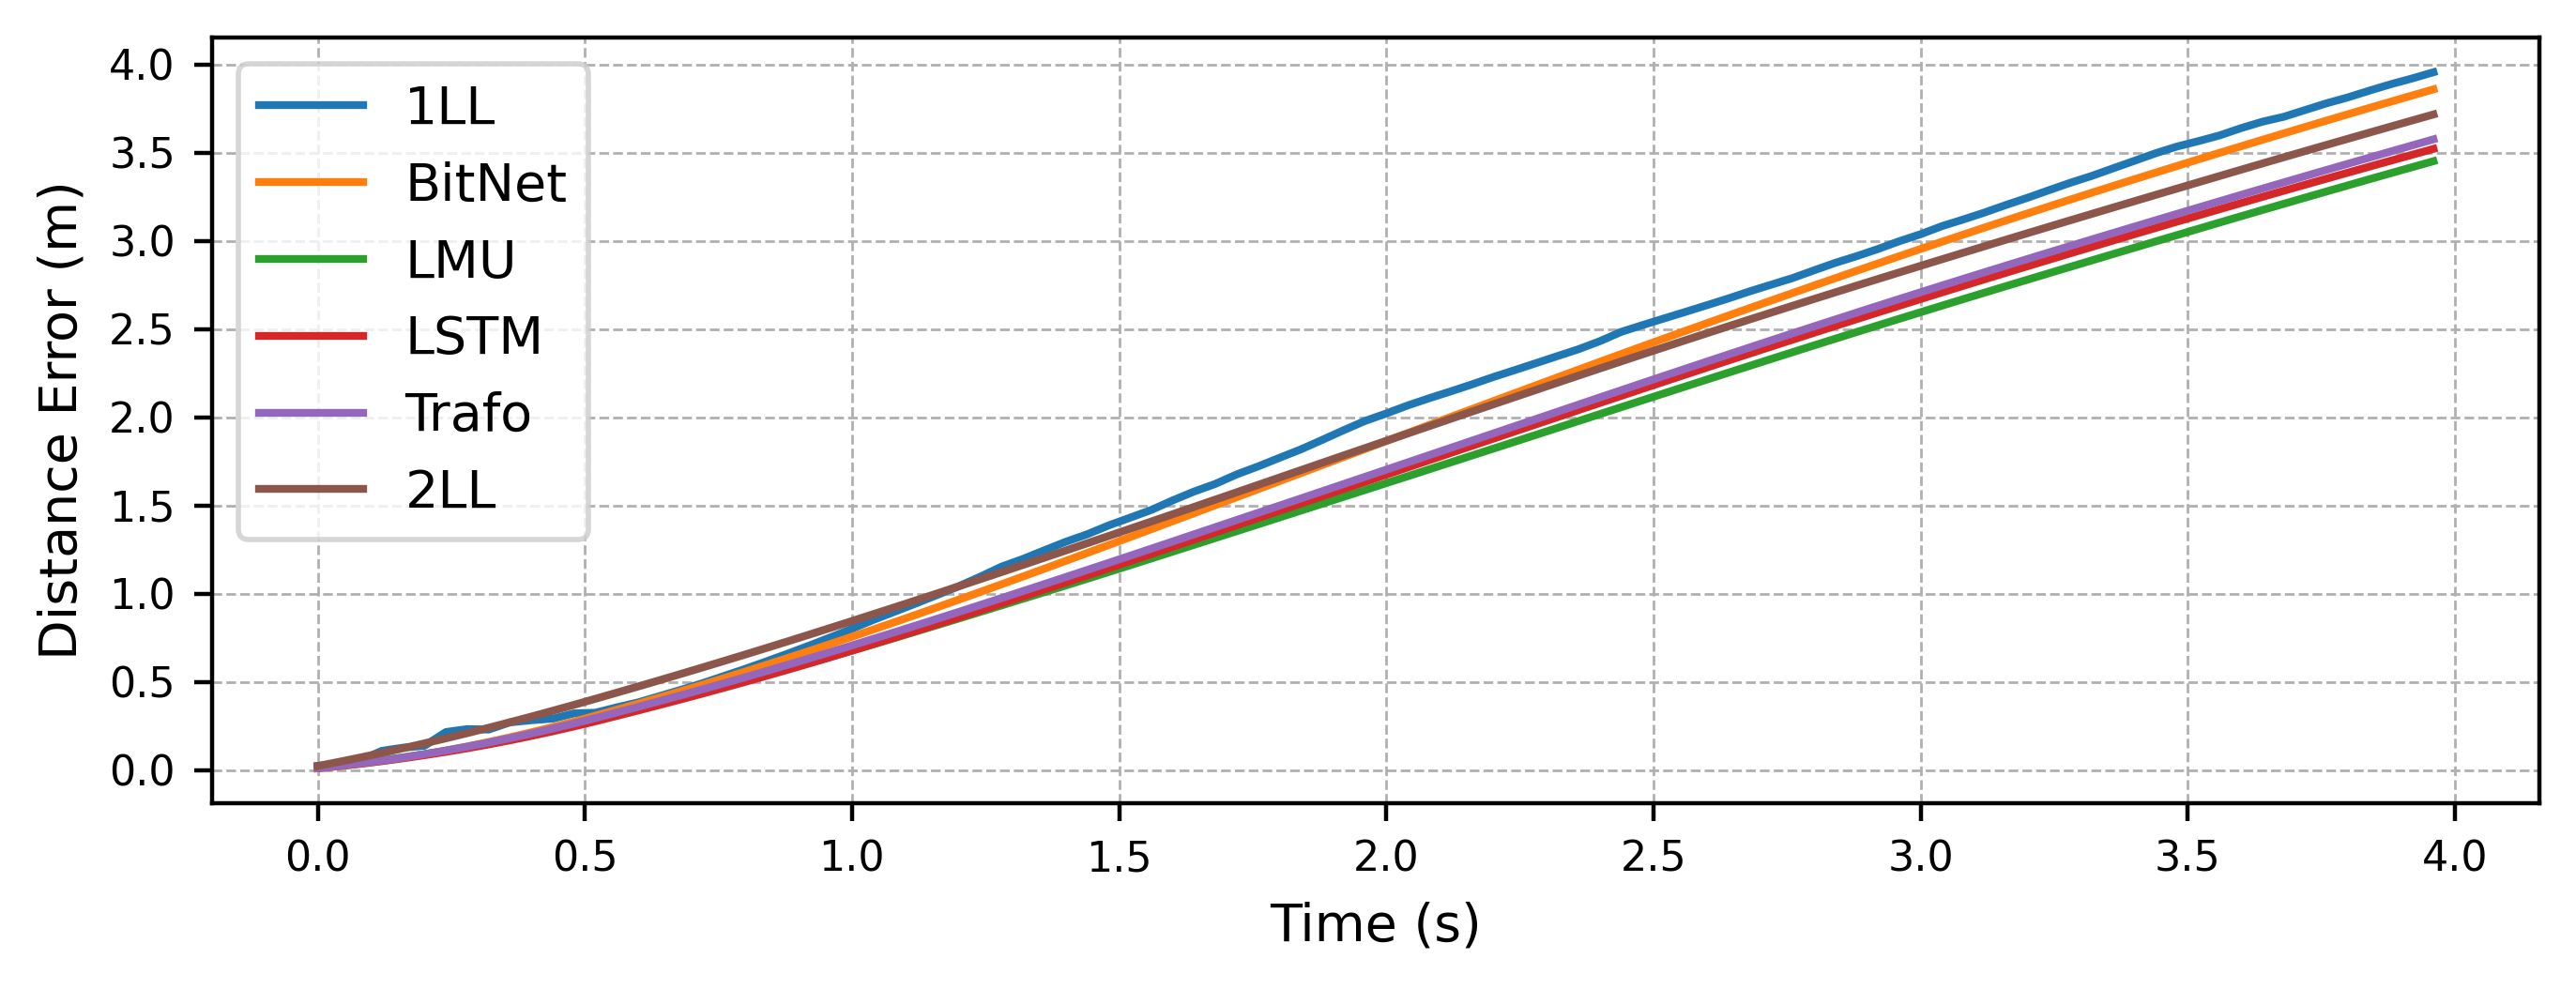
\includegraphics[width=\linewidth]{contents/results/nba_error.png}
    \caption[Distance Error Over Time (NBA).]{Plot showing the distance error over time for the NBA models, highlighting the performance trends of each model.}    \label{fig:distance_error_nba}
\end{figure}
\begin{figure}[t]
    \centering
    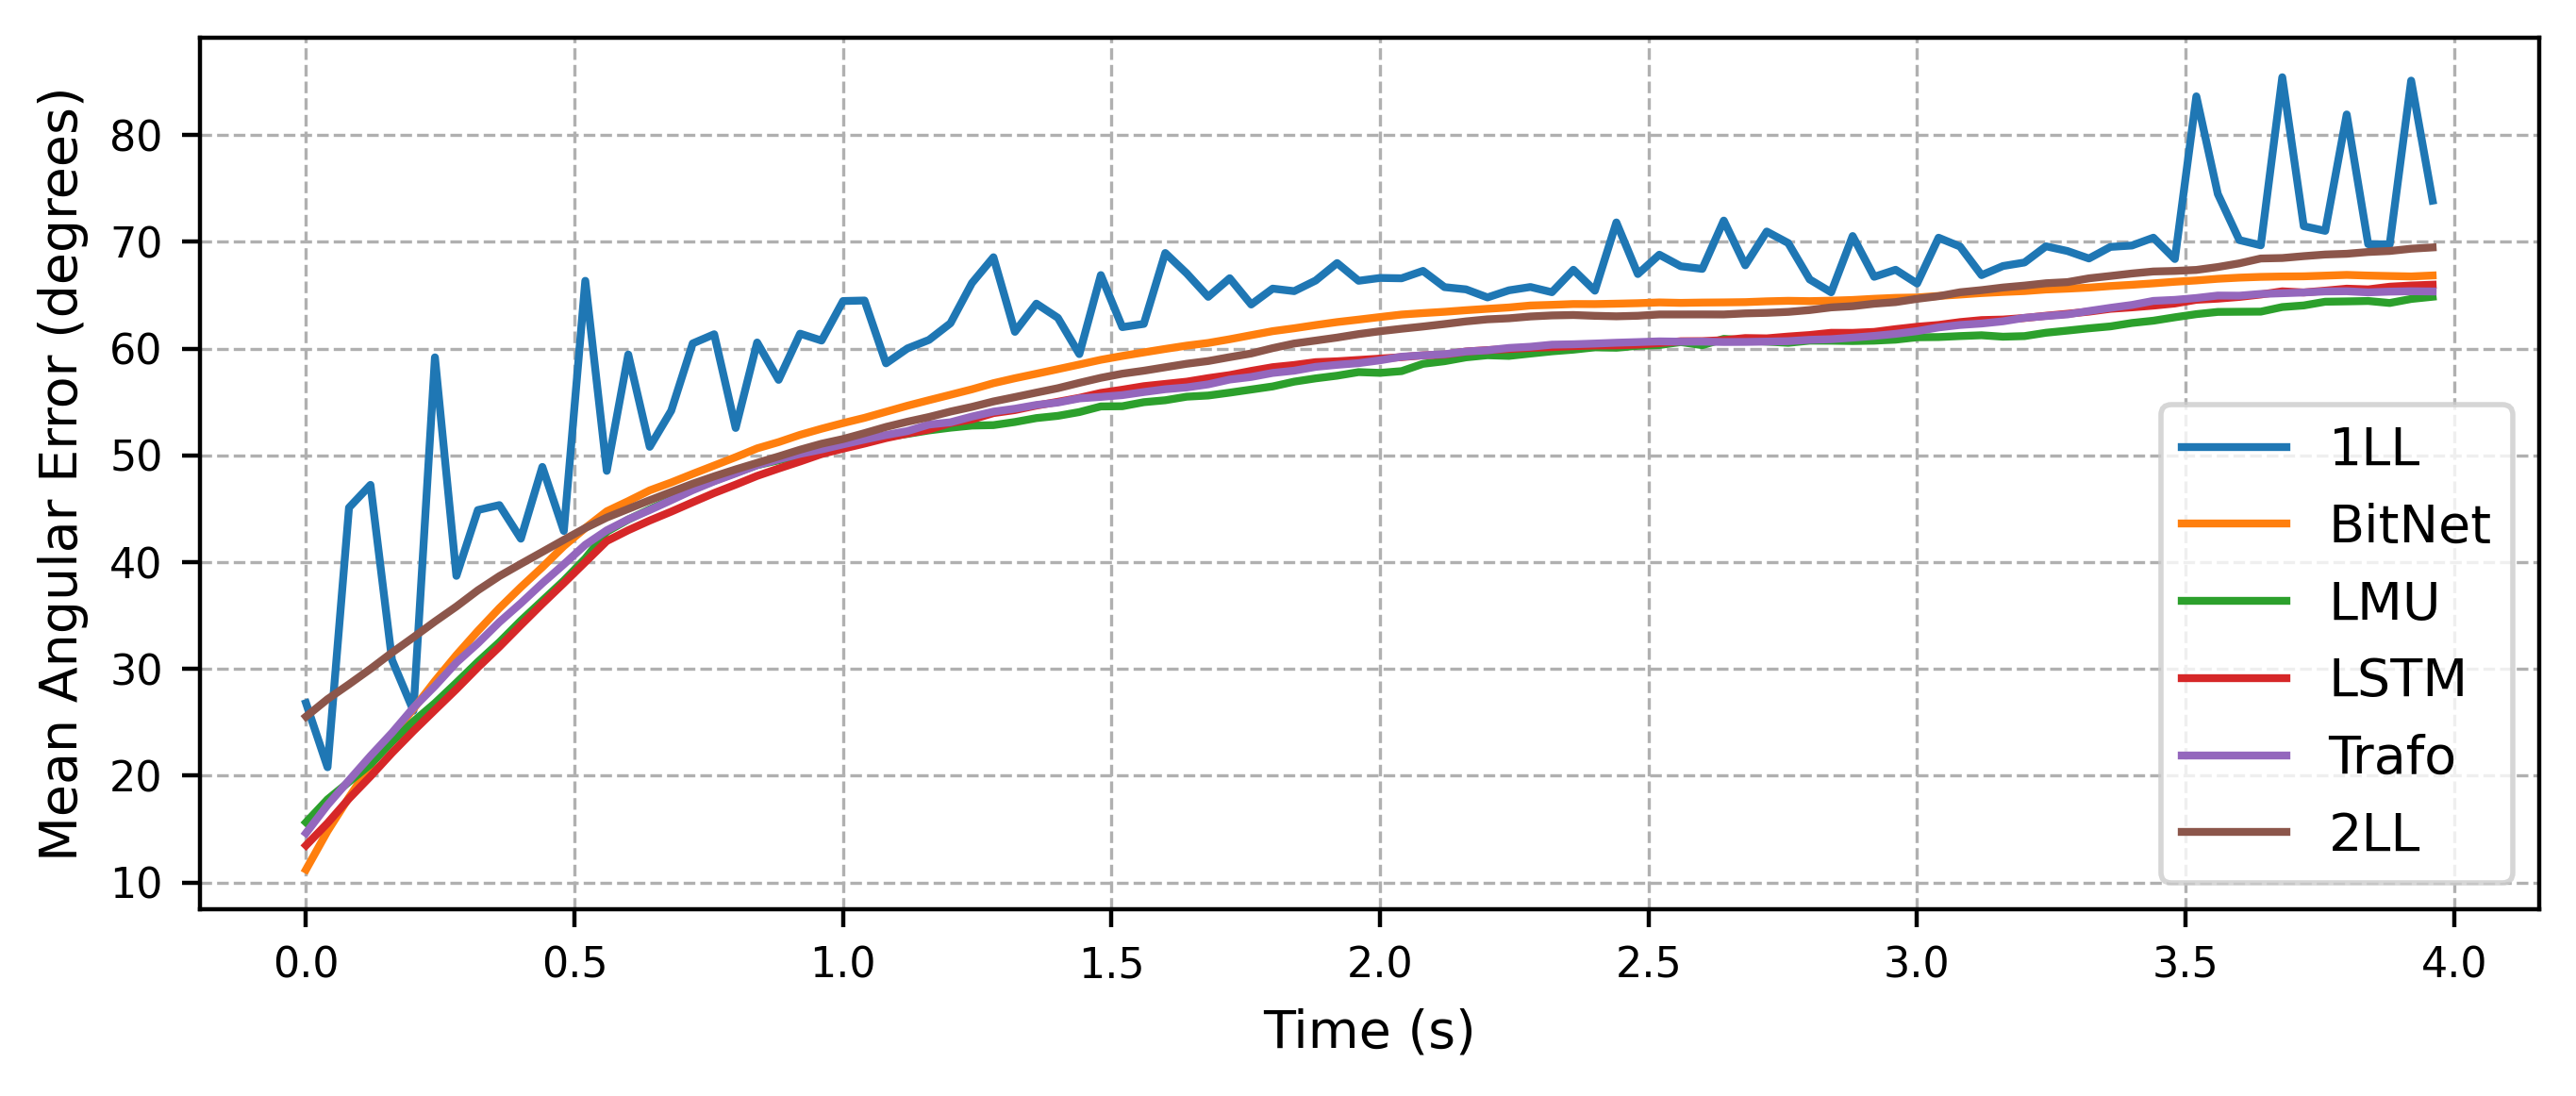
\includegraphics[width=\linewidth]{contents/results/nba_angle.png}
    \caption[Angular Error Over Time (NBA).]{Plot illustrating the angular error over time for the NBA models, demonstrating how well each model performs in this metric.}
    \label{fig:angular_error_nba}
\end{figure}
This section presents the results of Experiment E1 \ref{exp:e1} for the NBA and soccer datasets, revealing insights into the performance of attention-based models compared to established baseline models.
\paragraph{NBA Result:}

\begin{longtable}[t]{l|l||c|c|c|c|c|c}
\caption[Results of the first experiment (NBA).]{Results table for the NBA dataset, with the best scores highlighted in bold.} \label{tab:first_experiment_nba} \\

\hline
Metric & Statistic & 1L Linear & 2L Linear & BitNet & LMU & LSTM & Trafo \\
\hline\hline
\endfirsthead

\caption*{Continuation of Table \ref{tab:first_experiment_nba}} \\
\hline
Metric & Statistic & 1L Linear & 2L Linear & BitNet & LMU & LSTM & Trafo \\
\hline\hline
\endhead

\hline
\endfoot

\hline
AAE (\si{\text{grad}}) & Mean & 63.03 & 56.72 & 56.72 & \textbf{53.29} & 53.86 & 54.43 \\
 & Std & 52.14 & 50.99 & 50.99 & 49.85 & 50.42 & 50.42 \\
\hline
ADE (\si{\meter}) & Mean & 1.94 & 1.84 & 1.85 & \textbf{1.63} & 1.67 & 1.70 \\
 & Std & 1.17 & 1.23 & 1.19 & 1.11 & 1.13 & 1.16 \\
\hline
FAE (\si{\text{grad}}) & Mean & 73.91 & 69.33 & 67.04 & \textbf{64.74} & 65.89 & 65.32 \\
 & Std & 51.57 & 54.43 & 52.71 & 52.14 & 52.14 & 51.57 \\
\hline
FDE (\si{\meter}) & Mean & 3.96 & 3.72 & 3.86 & \textbf{3.45} & 3.52 & 3.58 \\
 & Std & 2.57 & 2.67 & 2.59 & 2.47 & 2.55 & 2.59 \\
\hline
MAE (\si{\meter}) & Mean & 1.23 & 1.16 & 1.17 & \textbf{1.03} & 1.06 & 1.08 \\
 & Std & 0.74 & 0.77 & 0.75 & 0.70 & 0.71 & 0.73 \\
\hline
MSE (\si{\meter}) & Mean & 3.76 & 3.57 & 3.60 & \textbf{2.92} & 3.06 & 3.18 \\
 & Std & 5.20 & 5.10 & 5.19 & 4.88 & 4.95 & 5.02 \\
\hline
NL\_ADE (\si{\meter}) & Mean & 2.34 & 2.35 & 2.36 & \textbf{2.14} & 2.18 & 2.21 \\
 & Std & 1.53 & 1.62 & 1.58 & 1.53 & 1.55 & 1.55 \\
\hline
\end{longtable}

\FloatBarrier

The results presented in Table \ref{tab:first_experiment_nba} indicate that the Transformer performed slightly worse than the RNN models across all metrics. Notably, the LMU outperformed the LSTM across all metrics in the NBA dataset, achieving an AAE of \SI{53.29}{\degree} and an ADE of \SI{1.63}{\meter}. This finding highlights the LMU's effectiveness in capturing the complexities of motion forecasting, which may stem from its ability to better model long-range dependencies compared to LSTM. In contrast, the Transformer achieved an AAE of \SI{54.43}{\degree} and an ADE of \SI{1.70}{\meter}, demonstrating that while attention-based models have potential, they still struggle with the inherent temporal dynamics of basketball, where rapid changes~occur.

Additionally, the linear models, including 1L Linear and 2L Linear, performed among the worst, with the 1L Linear model being particularly unstable as notable in the table for Mean Angular Error. The BitNet model also underperformed significantly across both datasets, which might be attributed to its limitation in encoding information using only binary values (0 and 1). This reduced capacity for nuanced information could hinder its effectiveness in the complex domain of human motion forecasting. Figures \ref{fig:distance_error_nba} and \ref{fig:angular_error_nba} illustrate the performance trends over prediction length, showing that all models exhibited a decline in accuracy as the prediction length increased, which aligns with expectations in the domain of human motion forecasting. This behavior underscores the challenges inherent in accurately predicting future positions over extended timeframes.

\newpage
\paragraph{Soccer Result:} 

\begin{figure}[t]
    \centering
    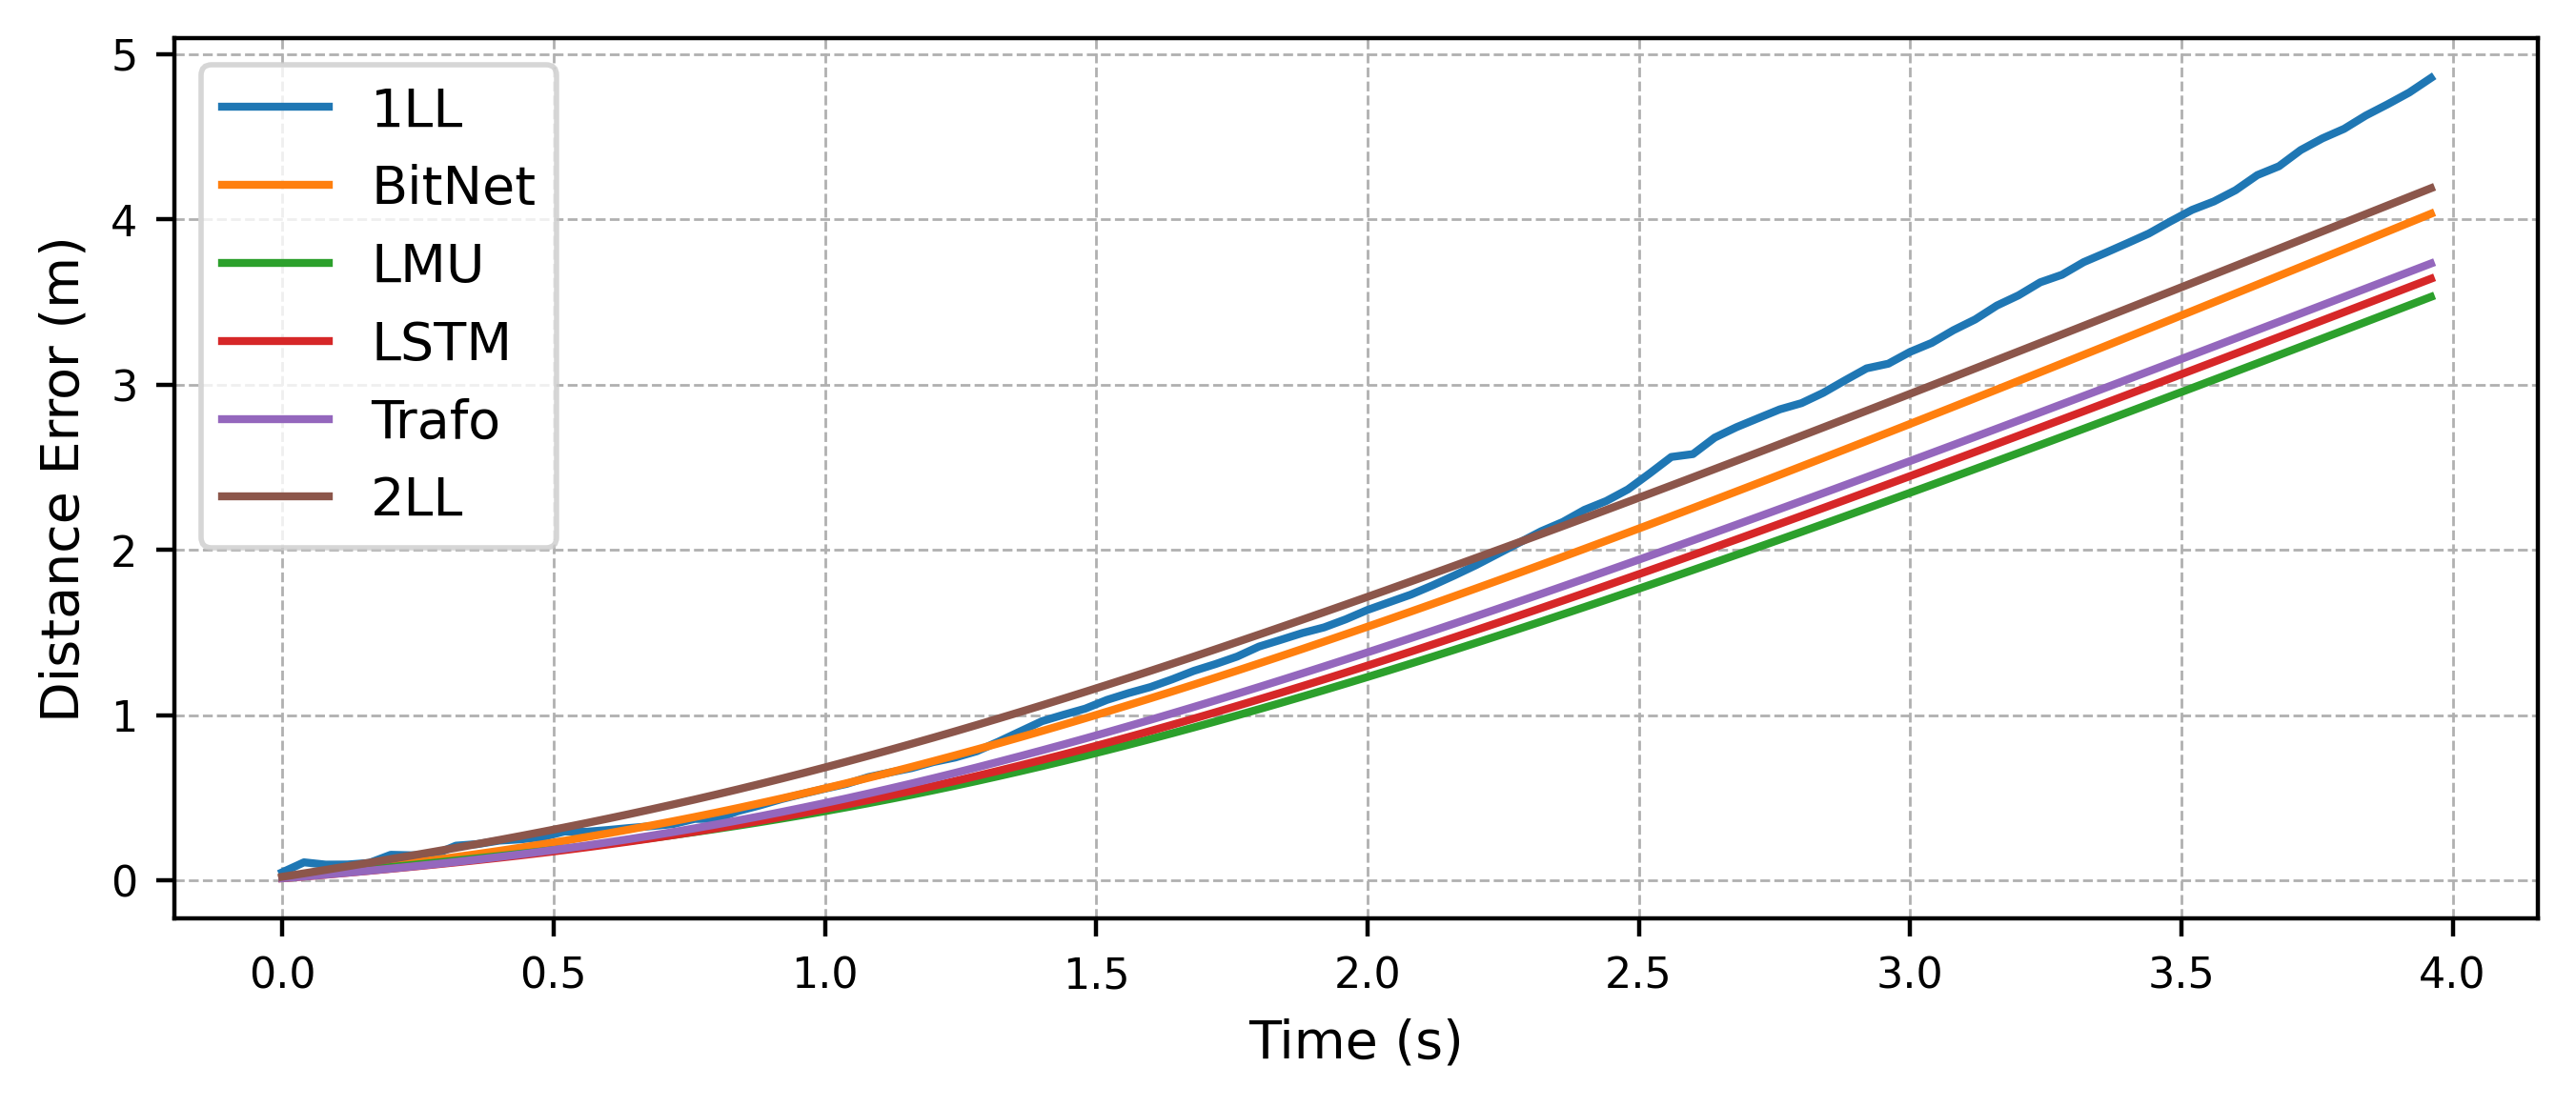
\includegraphics[width=\linewidth]{contents/results/soccer_error.png}
    \caption[Distance Error Over Time (DFL).]{Plot showing the distance error over time for the DFL models, highlighting the performance trends of each model.}
    \label{fig:distance_error_dfl}
\end{figure}
\begin{figure}[t]
    \centering
    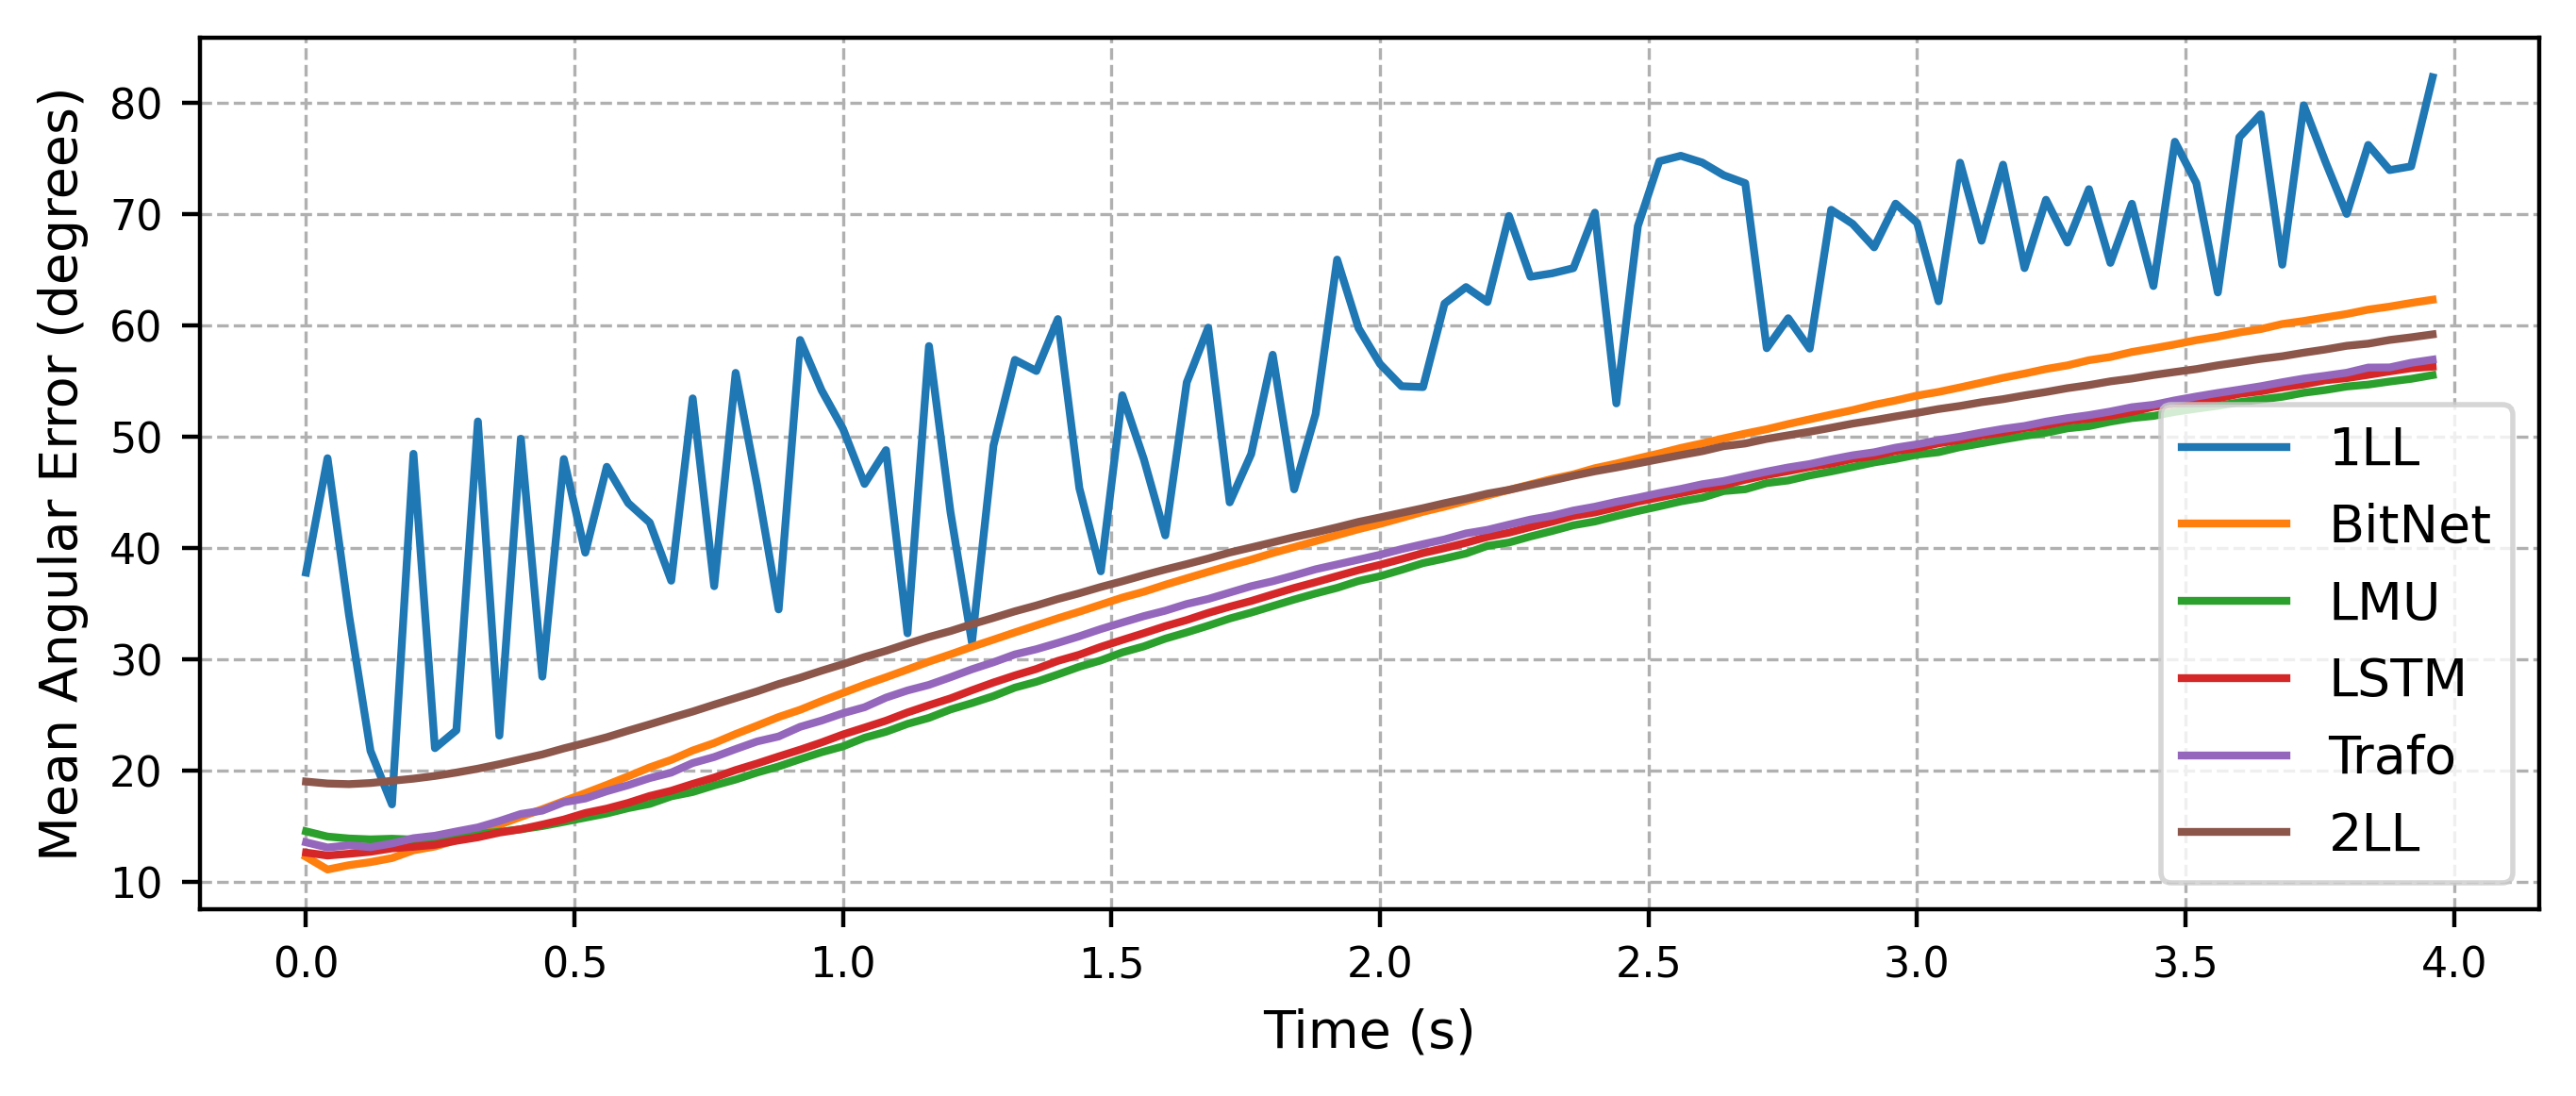
\includegraphics[width=\linewidth]{contents/results/soccer_angle.png}
    \caption[Angular Error Over Time (DFL).]{Plot illustrating the angular error over time for the DFL models, demonstrating how well each model performs in this metric.}
    \label{fig:angular_error_dfl}
\end{figure}


\begin{longtable}[t]{l|l||c|c|c|c|c|c}
\caption[Results of the first experiment (DFL).]{Results table for the DFL dataset, with the best scores highlighted in bold.} \label{tab:first_experiment_soccer} \\

\hline
Metric & Statistic & 1L Linear & 2L Linear & BitNet & LMU & LSTM & Trafo \\
\hline\hline
\endfirsthead

\caption*{Continuation of Table \ref{tab:first_experiment_soccer}} \\
\hline
Metric & Statistic & 1L Linear & 2L Linear & BitNet & LMU & LSTM & Trafo \\
\hline\hline
\endhead

\hline
\endfoot

\hline
AAE (\si{\text{grad}}) & Mean & 56.72 & 40.68 & 39.53 & \textbf{35.52} & 36.10 & 36.67 \\
 & Std & 47.56 & 42.97 & 43.54 & 41.25 & 41.83 & 41.83 \\
\hline
ADE (\si{\meter}) & Mean & 1.92 & 1.83 & 1.69 & \textbf{1.41} & 1.47 & 1.53 \\
 & Std & 1.15 & 1.29 & 1.34 & 1.02 & 1.14 & 1.17 \\
\hline
FAE (\si{\text{grad}}) & Mean & 82.51 & 59.01 & 62.45 & \textbf{55.58} & 56.15 & 56.72 \\
 & Std & 47.56 & 48.70 & 49.85 & 48.70 & 49.27 & 48.70 \\
\hline
FDE (\si{\meter}) & Mean & 4.85 & 4.19 & 4.03 & \textbf{3.53} & 3.64 & 3.73 \\
 & Std & 2.95 & 3.09 & 3.22 & 2.73 & 2.91 & 2.95 \\
\hline
MAE (\si{\meter}) & Mean & 1.23 & 1.16 & 1.07 & \textbf{0.90} & 0.93 & 0.97 \\
 & Std & 0.75 & 0.83 & 0.86 & 0.66 & 0.73 & 0.75 \\
\hline
MSE (\si{\meter}) & Mean & 4.12 & 3.85 & 3.68 & \textbf{2.53} & 2.84 & 3.01 \\
 & Std & 5.67 & 6.16 & 6.65 & 4.37 & 5.08 & 5.30 \\
\hline
NL\_ADE (\si{\meter}) & Mean & 2.03 & 1.99 & 1.90 & \textbf{1.62} & 1.72 & 1.76 \\
 & Std & 1.26 & 1.36 & 1.42 & 1.10 & 1.22 & 1.25 \\
\hline
\end{longtable}

\FloatBarrier

The results presented in Table \ref{tab:first_experiment_soccer} highlight the performance of various models on the DFL dataset. Notably, the LMU outperformed all other models, achieving an AAE of \SI{35.52}{\degree} and an ADE of \SI{1.41}{\meter}. This demonstrates its strong capability in accurately capturing the complexities of human motion in soccer. The Transformer model, while showing potential, achieved an AAE of \SI{36.67}{\degree} and an ADE of \SI{1.53}{\meter}, indicating that it performed slightly worse than the best RNN model, LMU, in this context. The performance gap between the LMU and the Transformer may be attributed to the latter's difficulty in leveraging temporal dependencies as effectively as RNNs, particularly in dynamic sports~scenarios.

In the soccer dataset, linear models again performed poorly, consistent with their behavior in the NBA dataset, and the BitNet struggled to compete, due to the same limitations in information encoding. Figures \ref{fig:distance_error_dfl} and \ref{fig:angular_error_dfl} illustrate the performance trends over prediction length for the soccer dataset, showing that all models exhibited a decline in accuracy as the prediction length increased, consistent with the challenges faced in accurately predicting future player positions in dynamic game scenarios.

\paragraph{Summary}
Overall, both datasets reveal common trends where RNN models, particularly the LMU, consistently outperform attention-based models including the Transformer. Additionally, linear models performed poorly across both datasets, with the 1L Linear model being very unstable and the BitNet model significantly underperforming due to its limitations in encoding information. These findings emphasize the need for further exploration into diverse architectures and input strategies in subsequent experiments (E2-E7) to enhance the performance of attention-based models in human motion forecasting.
\FloatBarrier


\begin{longtable}[H]{l|l||c|c|c|c|c|c}
\caption[Results of the second experiment excluding velocity information (NBA).]{Results table for the NBA dataset, showing the outcomes when velocity information is excluded from the experiment.} \label{tab:results_without_velocity_nba} \\

\hline
Metric & Statistic & 1L Linear & 2L Linear & BitNet & LMU & LSTM & Trafo \\
\hline\hline
\endfirsthead

\caption*{Continuation of Table \ref{tab:results_without_velocity_nba}} \\
\hline
Metric & Statistic & 1L Linear & 2L Linear & BitNet & LMU & LSTM & Trafo \\
\hline\hline
\endhead

\hline
\endfoot

\hline
AAE (\si{\text{grad}}) & Mean & 70.47 & 69.90 & 72.19 & 60.73 & \textbf{55.00} & 56.72 \\
 & Std & 52.14 & 55.58 & 55.58 & 50.42 & 49.85 & 50.42 \\
\hline
ADE (\si{\meter}) & Mean & 2.55 & 2.54 & 2.87 & 1.98 & \textbf{1.81} & 1.85 \\
 & Std & 1.54 & 1.63 & 1.59 & 1.29 & 1.22 & 1.24 \\
\hline
FAE (\si{\text{grad}}) & Mean & 75.63 & 73.91 & 75.06 & 67.04 & \textbf{64.17} & 65.89 \\
 & Std & 52.14 & 57.30 & 57.30 & 51.57 & 53.29 & 53.29 \\
\hline
FDE (\si{\meter}) & Mean & 4.57 & 4.57 & 5.17 & 3.81 & \textbf{3.60} & 3.64 \\
 & Std & 2.83 & 3.01 & 2.94 & 2.70 & 2.56 & 2.60 \\
\hline
MAE (\si{\meter}) & Mean & 1.61 & 1.59 & 1.79 & 1.25 & \textbf{1.14} & 1.17 \\
 & Std & 0.97 & 1.03 & 0.99 & 0.82 & 0.75 & 0.77 \\
\hline
MSE (\si{\meter}) & Mean & 5.84 & 6.02 & 7.06 & 3.91 & \textbf{3.40} & 3.53 \\
 & Std & 7.59 & 7.86 & 8.08 & 5.51 & 5.34 & 5.41 \\
\hline
NL\_ADE (\si{\meter}) & Mean & 2.91 & 2.99 & 3.21 & 2.44 & \textbf{2.30} & 2.35 \\
 & Std & 1.88 & 1.97 & 1.98 & 1.62 & 1.57 & 1.62 \\
\hline
\end{longtable}


\begin{longtable}[H]{l|l||c|c|c|c|c|c}
\caption[Results of the second experiment excluding position information (NBA).]{Results table for the NBA dataset, showing the outcomes when position information is excluded from the experiment.} \label{tab:results_without_position_nba} \\

\hline
Metric & Statistic & 1L Linear & 2L Linear & BitNet & LMU & LSTM & Trafo \\
\hline\hline
\endfirsthead

\caption*{Continuation of Table \ref{tab:results_without_position_nba}} \\
\hline
Metric & Statistic & 1L Linear & 2L Linear & BitNet & LMU & LSTM & Trafo \\
\hline\hline
\endhead

\hline
\endfoot

\hline
AAE (\si{\text{grad}}) & Mean & 62.45 & 61.88 & 80.79 & 61.88 & \textbf{59.01} & \textbf{59.01} \\
 & Std & 53.86 & 54.43 & 55.00 & 54.43 & 53.86 & 53.29 \\
\hline
ADE (\si{\meter}) & Mean & 1.96 & 1.94 & 2.87 & 1.86 & \textbf{1.78} & 1.81 \\
 & Std & 1.32 & 1.35 & 1.89 & 1.28 & 1.27 & 1.28 \\
\hline
FAE (\si{\text{grad}}) & Mean & 77.92 & 75.06 & 88.81 & 75.06 & 74.48 & \textbf{71.62} \\
 & Std & 55.00 & 55.00 & 52.71 & 56.15 & 56.15 & 55.00 \\
\hline
FDE (\si{\meter}) & Mean & 4.21 & 4.09 & 5.25 & 3.93 & \textbf{3.79} & 3.83 \\
 & Std & 3.01 & 3.04 & 3.81 & 2.92 & 2.88 & 2.88 \\
\hline
MAE (\si{\meter}) & Mean & 1.23 & 1.22 & 1.78 & 1.17 & \textbf{1.11} & 1.14 \\
 & Std & 0.83 & 0.84 & 1.15 & 0.80 & 0.78 & 0.79 \\
\hline
MSE (\si{\meter}) & Mean & 4.24 & 4.18 & 7.95 & 3.83 & \textbf{3.61} & 3.69 \\
 & Std & 5.86 & 6.12 & 10.30 & 5.70 & 5.52 & 5.68 \\
\hline
NL\_ADE (\si{\meter}) & Mean & 2.51 & 2.47 & 3.42 & 2.43 & 2.40 & \textbf{2.38} \\
 & Std & 1.82 & 1.82 & 2.39 & 1.80 & 1.79 & 1.75 \\
\hline
\end{longtable}

\subsection{E2: Evaluating Impact of Input Exclusions}
\label{exp:pos_vel}
This section presents the results of Experiment \textbf{E2: Evaluating Impact of Input Exclusions}. The focus of this experiment is to address the question \textbf{Q2: How does model performance vary when positional or velocity data is excluded?}
\paragraph {NBA Result:}
The results of Experiment E2 reveal how model performance is affected when either positional or velocity data is excluded from the input. Tables \ref{tab:results_without_velocity_nba} and \ref{tab:results_without_position_nba} present the outcomes for each condition.

\textbf{Excluding Velocity Information:} When velocity data is omitted, the results indicate a significant degradation in performance across all models, particularly in AAE and ADE metrics. The LMU still demonstrates competitive performance with an AAE of \SI{60.73}{\degree} and an ADE of \SI{1.98}{\meter}, but it is notably worse than when both data types are included. The LSTM achieves the best AAE with \SI{55.00}{\degree} and ADE of \SI{1.81}{\meter}, suggesting that retaining velocity data is crucial for achieving better accuracy in motion forecasting. The Transformer model follows closely, with an AAE of \SI{56.72}{\degree} and ADE of \SI{1.85}{\meter}, demonstrating its capability to compete with RNNs, albeit slightly lagging behind the LSTM. Linear models and BitNet show inferior performance, with BitNet being particularly poor, achieving an AAE of \SI{72.19}{\degree}, due to its limitations in capturing temporal dynamics with binary data representation.

\textbf{Excluding Position Information:} In contrast, excluding positional data results in a mixed performance across the models. The LSTM outperforms other models again with an AAE of \SI{59.01}{\degree} and an ADE of \SI{1.78}{\meter}. The Transformer achieves the same AAE of \SI{59.01}{\degree}, indicating its strong performance in this context. However, the BitNet exhibits an unexpected spike in AAE, achieving \SI{80.79}{\degree}, indicating that removing positional context severely hinders its ability to predict accurately. The LMU maintains a decent AAE of \SI{61.88}{\degree}, emphasizing its robustness, albeit with a drop in performance compared to full input conditions.

Overall, the results highlight that both positional and velocity data are essential for effective forecasting in human motion, with significant performance declines when either is excluded. The LSTM consistently demonstrates superior performance, closely followed by the Transformer, reinforcing the strength of RNNs and attention-based models in this context, while the LMU is outperformed by both in the NBA dataset. Notably, BitNet remains largely ineffective, being outperformed by simpler linear models, which suggests that its design may not be suited for this type of motion forecasting task.

\paragraph{Soccer Result:}
The results of Experiment E2 reveal how model performance is affected when either positional or velocity data is excluded from the input. Tables \ref{tab:results_without_velocity_soccer} and \ref{tab:results_without_position_soccer} present the outcomes for each condition.

\begin{longtable}[H]{l|l||c|c|c|c|c|c}
\caption[Results of the second experiment excluding velocity information (DFL).]{Results table for the DFL dataset, showing the outcomes when velocity information is excluded from the experiment. Best scores are highlighted in bold.} \label{tab:results_without_velocity_soccer} \\

\hline
Metric & Statistic & 1L Linear & 2L Linear & BitNet & LMU & LSTM & Trafo \\
\hline\hline
\endfirsthead

\caption*{Continuation of Table \ref{tab:results_without_velocity_soccer}} \\
\hline
Metric & Statistic & 1L Linear & 2L Linear & BitNet & LMU & LSTM & Trafo \\
\hline\hline
\endhead

\hline
\endfoot

\hline
AAE (\si{\text{grad}}) & Mean & 67.61 & 51.57 & 79.64 & 42.40 & 46.98 & \textbf{40.68} \\
 & Std & 50.99 & 48.13 & 53.86 & 43.54 & 45.26 & 43.54 \\
\hline
ADE (\si{\meter}) & Mean & 2.88 & 2.52 & 3.65 & 1.90 & 2.27 & \textbf{1.83} \\
 & Std & 1.88 & 1.86 & 2.38 & 1.36 & 1.68 & 1.44 \\
\hline
FAE (\si{\text{grad}}) & Mean & 73.91 & 67.04 & 75.06 & 60.73 & 61.88 & \textbf{59.01} \\
 & Std & 52.14 & 52.14 & 53.29 & 49.27 & 48.70 & 49.27 \\
\hline
FDE (\si{\meter}) & Mean & 5.81 & 5.21 & 6.92 & 4.23 & 4.80 & \textbf{4.18} \\
 & Std & 3.92 & 3.86 & 4.51 & 3.23 & 3.63 & 3.29 \\
\hline
MAE (\si{\meter}) & Mean & 1.84 & 1.59 & 2.30 & 1.21 & 1.44 & \textbf{1.16} \\
 & Std & 1.22 & 1.19 & 1.52 & 0.87 & 1.08 & 0.93 \\
\hline
MSE (\si{\meter}) & Mean & 8.35 & 6.87 & 12.52 & \textbf{4.12} & 5.72 & 4.13 \\
 & Std & 17.12 & 11.66 & 16.58 & 6.97 & 9.35 & 7.27 \\
\hline
NL\_ADE (\si{\meter}) & Mean & 2.98 & 2.66 & 3.76 & 2.06 & 2.42 & \textbf{2.05} \\
 & Std & 2.05 & 1.96 & 2.52 & 1.43 & 1.74 & 1.51 \\
\hline
\end{longtable}


\begin{longtable}[H]{l|l||c|c|c|c|c|c}
\caption[Results of the second experiment excluding position information (DFL).]{Results table for the DFL dataset, showing the outcomes when position information is excluded from the experiment. Best scores are highlighted in bold.} \label{tab:results_without_position_soccer} \\

\hline
Metric & Statistic & 1L Linear & 2L Linear & BitNet & LMU & LSTM & Trafo \\
\hline\hline
\endfirsthead

\caption*{Continuation of Table \ref{tab:results_without_position_soccer}} \\
\hline
Metric & Statistic & 1L Linear & 2L Linear & BitNet & LMU & LSTM & Trafo \\
\hline\hline
\endhead

\hline
\endfoot

\hline
AAE (\si{\text{grad}}) & Mean & 37.82 & 39.53 & 59.59 & 35.52 & \textbf{34.38} & 38.39 \\
 & Std & 42.40 & 42.97 & 49.27 & 41.25 & 41.25 & 42.97 \\
\hline
ADE (\si{\meter}) & Mean & 1.44 & 1.68 & 3.08 & 1.39 & \textbf{1.32} & 1.62 \\
 & Std & 1.08 & 1.21 & 2.01 & 1.04 & 1.02 & 1.22 \\
\hline
FAE (\si{\text{grad}}) & Mean & 65.89 & 63.60 & 72.77 & 58.44 & \textbf{57.30} & 60.16 \\
 & Std & 49.27 & 49.27 & 52.71 & 49.85 & 49.85 & 49.85 \\
\hline
FDE (\si{\meter}) & Mean & 3.83 & 4.12 & 5.99 & 3.60 & \textbf{3.49} & 3.93 \\
 & Std & 2.85 & 3.03 & 4.05 & 2.82 & 2.78 & 3.04 \\
\hline
MAE (\si{\meter}) & Mean & 0.92 & 1.07 & 1.96 & 0.88 & \textbf{0.84} & 1.03 \\
 & Std & 0.70 & 0.78 & 1.29 & 0.67 & 0.65 & 0.79 \\
\hline
MSE (\si{\meter}) & Mean & 2.82 & 3.47 & 9.14 & 2.58 & \textbf{2.42} & 3.31 \\
 & Std & 4.83 & 5.59 & 12.90 & 4.44 & 4.25 & 5.65 \\
\hline
NL\_ADE (\si{\meter}) & Mean & 1.69 & 1.89 & 3.18 & 1.63 & \textbf{1.59} & 1.83 \\
 & Std & 1.17 & 1.30 & 2.12 & 1.12 & 1.12 & 1.30 \\
\hline
\end{longtable}
\newpage

\textbf{Excluding Velocity Information:} When velocity data is omitted, the results indicate a significant drop in performance for the Transformer model, which achieves an AAE of \SI{40.68}{\degree} and an ADE of \SI{1.83}{\meter}. In contrast, the LSTM model stands out with the best performance metrics, demonstrating its ability to maintain accuracy even in the absence of velocity information, with an AAE of \SI{46.98}{\degree} and an ADE of \SI{2.27}{\meter}. Other models, such as BitNet and LMU, show considerable degradation in performance, particularly in AAE and ADE metrics. The LMU's performance (AAE of \SI{42.40}{\degree}, ADE of \SI{1.90}{\meter}) also emphasizes the importance of velocity data for effective forecasting.

\textbf{Excluding Position Information:} In contrast, excluding positional data results in a noteworthy performance increase for the LSTM model, which achieves the best metrics with an AAE of \SI{34.38}{\degree} and an ADE of \SI{1.32}{\meter}. This performance boost can be attributed to the LSTM's inherent design, which leverages sequential data and temporal dependencies effectively. In the absence of positional context, the LSTM's ability to model temporal patterns allows it to focus more on velocity dynamics, resulting in improved performance. The Transformer, while performing competitively with an AAE of \SI{38.39}{\degree}, still falls short compared to the LSTM. Notably, the BitNet experiences a significant decline in performance, achieving an AAE of \SI{59.59}{\degree}, highlighting its reliance on positional information for accurate predictions. The LMU also maintains decent performance with an AAE of \SI{35.52}{\degree}, underscoring its robustness despite the lack of positional context.

\paragraph{Summary:} The results from both basketball and soccer datasets highlight the necessity of both positional and velocity data for effective motion forecasting. In the soccer dataset, both recurrent models (LSTM and LMU) outperformed those using the full input context when positional data was absent, as they could concentrate better on velocity dynamics, leading to enhanced accuracy. This ability to focus on velocities resulted in a notable performance increase compared to models reliant on both data types. The Transformer remains a competitive option but does not consistently outperform the recurrent models. In contrast, both BitNet and linear models underperform significantly, indicating their inadequacies in capturing the complexities of motion dynamics, with BitNet particularly noted as ineffective for these tasks. Overall, these findings illustrate the varying strengths of different modeling approaches in human motion forecasting.

\FloatBarrier
\subsection{Historical Context and Forecast Horizon}
\label{exp:history_forcast}

This section presents the results of Experiment \textbf{E3: Robustness to Missing Historical Information} \ref{exp:e3}. The focus of this experiment is to address the question \textbf{Q3: How robust is each model to missing historical information?}
\paragraph {NBA Result:}

\begin{longtable}[t]{l|l||c|c|c|c|c|c}
\caption[Results for $0.04\si{\second}$ historical context (NBA).]{Results table for the NBA dataset using a $0.04\si{\second}$ historical context, with the best scores highlighted in bold.} \label{tab:results_0.04s_nba} \\

\hline
Metric & Statistic & 1L Linear & 2L Linear & BitNet & LMU & LSTM & Trafo \\
\hline\hline
\endfirsthead

\caption*{Continuation of Table \ref{tab:results_0.04s_nba}} \\
\hline
Metric & Statistic & 1L Linear & 2L Linear & BitNet & LMU & LSTM & Trafo \\
\hline\hline
\endhead

\hline
\endfoot

\hline
AAE (\si{\text{grad}}) & Mean & 57.87 & \textbf{55.58} & 57.87 & 68.18 & 58.44 & 56.15 \\
 & Std & 51.57 & 50.42 & 51.57 & 53.86 & 51.57 & 50.42 \\
\hline
ADE (\si{\meter}) & Mean & 1.89 & \textbf{1.76} & 1.98 & 3.31 & 1.93 & 1.83 \\
 & Std & 1.24 & 1.20 & 1.25 & 1.57 & 1.25 & 1.28 \\
\hline
FAE (\si{\text{grad}}) & Mean & 68.18 & \textbf{67.04} & 68.75 & 77.35 & 69.33 & \textbf{67.04} \\
 & Std & 52.14 & 52.14 & 53.29 & 55.00 & 53.86 & 51.57 \\
\hline
FDE (\si{\meter}) & Mean & 3.95 & \textbf{3.65} & 4.06 & 6.40 & 3.95 & 3.80 \\
 & Std & 2.67 & 2.64 & 2.64 & 3.18 & 2.64 & 2.81 \\
\hline
MAE (\si{\meter}) & Mean & 1.19 & \textbf{1.11} & 1.25 & 2.06 & 1.21 & 1.15 \\
 & Std & 0.77 & 0.74 & 0.77 & 0.94 & 0.76 & 0.80 \\
\hline
MSE (\si{\meter}) & Mean & 3.80 & \textbf{3.37} & 4.00 & 9.30 & 3.84 & 3.70 \\
 & Std & 5.50 & 5.43 & 5.95 & 9.22 & 5.71 & 5.67 \\
\hline
NL\_ADE (\si{\meter}) & Mean & 2.38 & \textbf{2.21} & 2.37 & 3.58 & 2.34 & 2.34 \\
 & Std & 1.63 & 1.59 & 1.61 & 2.27 & 1.60 & 1.68 \\
\hline
\end{longtable}


\begin{longtable}[t]{l|l||c|c|c|c|c|c}
\caption[Results for $0.40\si{\second}$ historical context (NBA).]{Results table for the NBA dataset using a $0.40\si{\second}$ historical context, with the best scores highlighted in bold.} \label{tab:results_0.4s_nba} \\

\hline
Metric & Statistic & 1L Linear & 2L Linear & BitNet & LMU & LSTM & Trafo \\
\hline\hline
\endfirsthead

\caption*{Continuation of Table \ref{tab:results_0.4s_nba}} \\
\hline
Metric & Statistic & 1L Linear & 2L Linear & BitNet & LMU & LSTM & Trafo \\
\hline\hline
\endhead

\hline
\endfoot

\hline
AAE (\si{\text{grad}}) & Mean & 59.59 & 56.72 & 57.30 & \textbf{55.00} & \textbf{55.00} & 55.58 \\
 & Std & 52.71 & 51.57 & 50.99 & 50.42 & 50.42 & 50.42 \\
\hline
ADE (\si{\meter}) & Mean & 1.90 & 1.79 & 1.89 & \textbf{1.70} & \textbf{1.70} & 1.78 \\
 & Std & 1.22 & 1.21 & 1.24 & 1.20 & 1.20 & 1.24 \\
\hline
FAE (\si{\text{grad}}) & Mean & 69.33 & 67.61 & 67.61 & 66.46 & \textbf{65.89} & 66.46 \\
 & Std & 53.86 & 53.29 & 52.71 & 52.71 & 52.14 & 51.57 \\
\hline
FDE (\si{\meter}) & Mean & 3.98 & 3.72 & 3.92 & \textbf{3.55} & 3.59 & 3.74 \\
 & Std & 2.61 & 2.66 & 2.65 & 2.64 & 2.67 & 2.75 \\
\hline
MAE (\si{\meter}) & Mean & 1.20 & 1.12 & 1.19 & \textbf{1.07} & \textbf{1.07} & 1.12 \\
 & Std & 0.76 & 0.75 & 0.76 & 0.74 & 0.74 & 0.77 \\
\hline
MSE (\si{\meter}) & Mean & 3.78 & 3.46 & 3.76 & \textbf{3.23} & 3.26 & 3.53 \\
 & Std & 5.42 & 5.33 & 5.62 & 5.70 & 5.46 & 5.48 \\
\hline
NL\_ADE (\si{\meter}) & Mean & 2.38 & 2.25 & 2.36 & \textbf{2.15} & 2.18 & 2.30 \\
 & Std & 1.60 & 1.61 & 1.63 & 1.60 & 1.62 & 1.65 \\
\hline
\end{longtable}


\begin{longtable}[t]{l|l||c|c|c|c|c|c}
\caption[Results for $1.00\si{\second}$ historical context (NBA).]{Results table for the NBA dataset using a $1.00\si{\second}$ historical context, with the best scores highlighted in bold.} \label{tab:results_1s_nba} \\

\hline
Metric & Statistic & 1L Linear & 2L Linear & BitNet & LMU & LSTM & Trafo \\
\hline\hline
\endfirsthead

\caption*{Continuation of Table \ref{tab:results_1s_nba}} \\
\hline
Metric & Statistic & 1L Linear & 2L Linear & BitNet & LMU & LSTM & Trafo \\
\hline\hline
\endhead

\hline
\endfoot

\hline
AAE (\si{\text{grad}}) & Mean & 61.31 & 56.72 & 56.72 & \textbf{53.86} & 54.43 & 55.00 \\
 & Std & 52.14 & 50.42 & 50.99 & 50.42 & 50.42 & 50.42 \\
\hline
ADE (\si{\meter}) & Mean & 1.88 & 1.83 & 1.87 & \textbf{1.65} & 1.69 & 1.74 \\
 & Std & 1.20 & 1.22 & 1.22 & 1.15 & 1.17 & 1.20 \\
\hline
FAE (\si{\text{grad}}) & Mean & 85.94 & 67.04 & 67.04 & \textbf{65.89} & \textbf{65.89} & \textbf{65.89} \\
 & Std & 56.15 & 52.71 & 52.71 & 52.14 & 51.57 & 51.57 \\
\hline
FDE (\si{\meter}) & Mean & 4.02 & 3.77 & 3.90 & \textbf{3.49} & 3.57 & 3.66 \\
 & Std & 2.58 & 2.72 & 2.64 & 2.56 & 2.63 & 2.69 \\
\hline
MAE (\si{\meter}) & Mean & 1.19 & 1.16 & 1.18 & \textbf{1.04} & 1.07 & 1.10 \\
 & Std & 0.75 & 0.76 & 0.75 & 0.71 & 0.72 & 0.75 \\
\hline
MSE (\si{\meter}) & Mean & 3.72 & 3.58 & 3.69 & \textbf{3.05} & 3.18 & 3.36 \\
 & Std & 5.22 & 5.33 & 5.43 & 5.24 & 5.19 & 5.24 \\
\hline
NL\_ADE (\si{\meter}) & Mean & 2.37 & 2.32 & 2.36 & \textbf{2.14} & 2.19 & 2.25 \\
 & Std & 1.63 & 1.65 & 1.62 & 1.57 & 1.59 & 1.62 \\
\hline
\end{longtable}


The performance of various models on forecasting human motion in basketball was assessed by analyzing their robustness to different historical input lengths. The following insights summarize the findings for each historical context evaluated:

\textbf{0.04 Seconds Historical Context:} In this scenario, the 2L Linear model outperformed all other models, achieving the lowest ADE and AAE. This surprising result indicates that the 2L Linear model effectively captures the dynamics of motion with minimal historical input. The attention-based Transformer model also demonstrated competitive performance, being the closest contender to the 2L Linear model. In contrast, the BitNet model struggled, as did the recurrent models, which faced challenges due to their reliance on longer historical sequences. With only one sample of history available, these models could not compete effectively in this short context. (See Table~\ref{tab:results_0.04s_nba}.)

\textbf{0.4 Seconds Historical Context:} As the historical context was increased to \SI{0.4}{\second}, the BitNet model showed improvement but still could not compete. The LMU improved drastically, moving from the worst-behaved model to being competitive alongside the LSTM. The Transformer model also gained a very small improvement with the longer context and could still compete with the leading models. The linear models were outperformed and lagged behind. Similar to the LMU, the LSTM improved drastically with the longer input. (See Table~\ref{tab:results_0.4s_nba}.)

\textbf{1.0 Seconds Historical Context:} With a historical context of \SI{1.0}{\second}, model performance, while not significantly increasing the metrics, still showed improvements in all metrics. Notably, the linear models suffered from longer historical input, as they lack a concept of time and how it flows, seeing all information at once. The BitNet maintained its poor performance. (See Table~\ref{tab:results_1s_nba}.)

The results suggest that each model behaves differently depending on the length of historical information. Linear models performed best with short inputs, while RNNs require longer context information to achieve better performance. It is also noteworthy that linear models cannot compete with the other models when the correct history length is selected. The Transformer model handles missing context better than the other models, remaining stable across all variants while still performing quite well in each scenario, meaning it can extract the necessary information needed to predict the future effectively.

\FloatBarrier
\paragraph {Soccer Result:}
The evaluation of model performance for forecasting human motion in soccer focused on their robustness across varying historical input lengths. The insights below summarize the key findings for each historical context assessed:

\textbf{0.04 Seconds Historical Context:} For the smallest historical context, the linear models emerged as the best predictors, particularly the 2L Linear model, which achieved an ADE of \SI{1.78}{\meter}. In this setting, the LMU once again performed poorly, registering the worst ADE of \SI{3.20}{\meter}. The LSTM model also struggled with the short history, while the Transformer remained competitive, attaining an ADE of \SI{1.83}{\meter}. (See Table~\ref{tab:results_0.04s_soccer}.)

\textbf{0.4 Seconds Historical Context:} Surprisingly, in the context of soccer, the linear models continued to perform competitively even with a historical input length of \SI{0.4}{\second}. This duration may be manageable for linear models without causing confusion. Although other models came close, they did not consistently surpass the linear models in this scenario. The Transformer model remained competitive with the 1L and 2L Linear models, while the recurrent models generally lagged behind, with the LSTM's performance deteriorating, due to misleading short and quick changes in player movements. Notably, the BitNet model outperformed both RNN models, achieving an ADE of \SI{1.79}{\meter}. (See Table~\ref{tab:results_0.4s_soccer}.)

\textbf{1.0 Seconds Historical Context:} With a historical context of \SI{1.0}{\second}, model performance aligned more closely with expectations. The LSTM and Transformer emerged as the leaders, exhibiting similar performance metrics. Following them was the BitNet, which, while significantly behind the leaders, still ranked third, slightly ahead of the linear models. Despite improvements from shorter histories, the LMU surprisingly retained its status as the worst performer in this context. (See Table~\ref{tab:results_1s_soccer}.)

The summary of the results indicates that input length is critical for model performance. As anticipated, all models showed improved performance with more historical information. Interestingly, unlike in the NBA, the linear models also enhanced their performance with longer histories in soccer, suggesting that this sport may be easier to learn and less dynamic than basketball. Notably, the Transformer maintained competitive performance across all contexts, demonstrating stability even if it did not always lead in specific metrics. The LMU's failure to compete in shorter historical contexts, performing best only with a full history length of \SI{2.0}{\second}, further emphasizes the importance of context length.

\begin{longtable}[H]{l|l||c|c|c|c|c|c}
\caption[Results for $0.04\si{\second}$ historical context (DFL).]{Results table for the DFL dataset using a $0.04\si{\second}$ historical context, with the best scores highlighted in bold.} \label{tab:results_0.04s_soccer} \\

\hline
Metric & Statistic & 1L Linear & 2L Linear & BitNet & LMU & LSTM & Trafo \\
\hline\hline
\endfirsthead

\caption*{Continuation of Table \ref{tab:results_0.04s_soccer}} \\
\hline
Metric & Statistic & 1L Linear & 2L Linear & BitNet & LMU & LSTM & Trafo \\
\hline\hline
\endhead

\hline
\endfoot

\hline
AAE (\si{\text{grad}}) & Mean & 42.40 & \textbf{41.83} & 42.40 & 50.42 & 44.12 & 42.97 \\
 & Std & 45.26 & 44.69 & 44.69 & 46.98 & 45.26 & 45.84 \\
\hline
ADE (\si{\meter}) & Mean & 1.82 & \textbf{1.78} & 2.15 & 3.20 & 2.18 & 1.86 \\
 & Std & 1.40 & 1.38 & 1.58 & 1.45 & 1.56 & 1.43 \\
\hline
FAE (\si{\text{grad}}) & Mean & 64.74 & \textbf{61.31} & 63.60 & 64.17 & 63.60 & 63.03 \\
 & Std & 51.57 & 48.70 & 49.85 & 51.57 & 50.99 & 50.99 \\
\hline
FDE (\si{\meter}) & Mean & 4.33 & \textbf{4.24} & 4.64 & 7.18 & 4.65 & 4.35 \\
 & Std & 3.32 & 3.29 & 3.59 & 3.59 & 3.39 & 3.41 \\
\hline
MAE (\si{\meter}) & Mean & 1.16 & \textbf{1.13} & 1.36 & 2.02 & 1.38 & 1.18 \\
 & Std & 0.89 & 0.88 & 1.01 & 0.93 & 1.00 & 0.91 \\
\hline
MSE (\si{\meter}) & Mean & 4.14 & \textbf{4.01} & 5.23 & 9.28 & 5.13 & 4.30 \\
 & Std & 6.94 & 6.83 & 8.93 & 9.06 & 7.92 & 7.38 \\
\hline
NL\_ADE (\si{\meter}) & Mean & 2.04 & \textbf{2.00} & 2.29 & 3.24 & 2.33 & 2.05 \\
 & Std & 1.47 & 1.45 & 1.65 & 1.69 & 1.65 & 1.49 \\
\hline
\end{longtable}


\begin{longtable}[H]{l|l||c|c|c|c|c|c}
\caption[Results for $0.40\si{\second}$ historical context (DFL).]{Results table for the DFL dataset using a $0.40\si{\second}$ historical context, with the best scores highlighted in bold.} \label{tab:results_0.4s_soccer} \\

\hline
Metric & Statistic & 1L Linear & 2L Linear & BitNet & LMU & LSTM & Trafo \\
\hline\hline
\endfirsthead

\caption*{Continuation of Table \ref{tab:results_0.4s_soccer}} \\
\hline
Metric & Statistic & 1L Linear & 2L Linear & BitNet & LMU & LSTM & Trafo \\
\hline\hline
\endhead

\hline
\endfoot

\hline
AAE (\si{\text{grad}}) & Mean & 42.40 & 40.68 & 40.68 & 42.40 & 57.30 & \textbf{40.11} \\
 & Std & 44.69 & 43.54 & 44.12 & 43.54 & 52.14 & 44.12 \\
\hline
ADE (\si{\meter}) & Mean & \textbf{1.64} & 1.77 & 1.79 & 3.10 & 2.35 & 1.69 \\
 & Std & 1.13 & 1.30 & 1.43 & 1.70 & 1.46 & 1.29 \\
\hline
FAE (\si{\text{grad}}) & Mean & 68.18 & \textbf{60.16} & 63.03 & 61.31 & 72.77 & \textbf{60.16} \\
 & Std & 50.42 & 50.42 & 49.85 & 50.42 & 52.14 & 49.85 \\
\hline
FDE (\si{\meter}) & Mean & 4.21 & 4.11 & 4.17 & 5.80 & 5.25 & \textbf{4.04} \\
 & Std & 2.96 & 3.10 & 3.36 & 3.70 & 3.45 & 3.16 \\
\hline
MAE (\si{\meter}) & Mean & \textbf{1.04} & 1.12 & 1.14 & 1.95 & 1.47 & 1.07 \\
 & Std & 0.73 & 0.84 & 0.92 & 1.07 & 0.92 & 0.82 \\
\hline
MSE (\si{\meter}) & Mean & \textbf{3.35} & 3.74 & 4.07 & 8.53 & 5.83 & 3.60 \\
 & Std & 5.25 & 6.21 & 7.38 & 9.90 & 7.63 & 6.18 \\
\hline
NL\_ADE (\si{\meter}) & Mean & \textbf{1.83} & 1.95 & 2.00 & 3.16 & 2.47 & 1.90 \\
 & Std & 1.22 & 1.37 & 1.50 & 1.80 & 1.56 & 1.36 \\
\hline
\end{longtable}


\begin{longtable}[H]{l|l||c|c|c|c|c|c}
\caption[Results for $1.00\si{\second}$ historical context (DFL).]{Results table for the DFL dataset using a $1.00\si{\second}$ historical context, with the best scores highlighted in bold.} \label{tab:results_1s_soccer} \\

\hline
Metric & Statistic & 1L Linear & 2L Linear & BitNet & LMU & LSTM & Trafo \\
\hline\hline
\endfirsthead

\caption*{Continuation of Table \ref{tab:results_1s_soccer}} \\
\hline
Metric & Statistic & 1L Linear & 2L Linear & BitNet & LMU & LSTM & Trafo \\
\hline\hline
\endhead

\hline
\endfoot

\hline
AAE (\si{\text{grad}}) & Mean & 48.70 & 39.53 & 39.53 & 42.97 & \textbf{37.24} & 37.82 \\
 & Std & 45.84 & 42.97 & 43.54 & 44.12 & 41.83 & 42.40 \\
\hline
ADE (\si{\meter}) & Mean & 1.75 & 1.74 & 1.71 & 2.00 & \textbf{1.56} & 1.57 \\
 & Std & 1.14 & 1.30 & 1.37 & 1.37 & 1.18 & 1.20 \\
\hline
FAE (\si{\text{grad}}) & Mean & 67.04 & 59.59 & 61.88 & 59.59 & \textbf{57.87} & \textbf{57.87} \\
 & Std & 50.42 & 49.85 & 49.85 & 49.27 & 48.70 & 49.27 \\
\hline
FDE (\si{\meter}) & Mean & 4.23 & 4.06 & 4.05 & 4.53 & 3.82 & \textbf{3.80} \\
 & Std & 2.92 & 3.13 & 3.27 & 3.21 & 2.96 & 3.01 \\
\hline
MAE (\si{\meter}) & Mean & 1.12 & 1.10 & 1.08 & 1.28 & \textbf{0.99} & \textbf{0.99} \\
 & Std & 0.74 & 0.84 & 0.88 & 0.90 & 0.76 & 0.77 \\
\hline
MSE (\si{\meter}) & Mean & 3.57 & 3.68 & 3.77 & 4.52 & \textbf{3.11} & 3.15 \\
 & Std & 5.38 & 6.20 & 6.88 & 6.93 & 5.31 & 5.54 \\
\hline
NL\_ADE (\si{\meter}) & Mean & 1.90 & 1.93 & 1.92 & 2.16 & 1.80 & \textbf{1.79} \\
 & Std & 1.24 & 1.37 & 1.44 & 1.50 & 1.25 & 1.27 \\
\hline
\end{longtable}

\paragraph{Summary} The results of Experiment \textbf{E3} indicate that the length of historical context is crucial for model performance. Linear models generally excel with shorter histories, while RNNs and attention-based models show significantly improved performance with longer contexts, surpassing the linear models in these scenarios. Notably, the Transformer model demonstrated consistent stability across all historical lengths in both datasets. In contrast, the BitNet model consistently underperformed throughout the evaluations.


\subsection{E4: Comparing Univariate and Multivariate Predictors}
\label{exp:uni_multi}

This section addresses Question \textbf{Q4: How does a multivariate predictor compare to multiple univariate pre-
dictors in terms of forecasting accuracy?} through Experiment \textbf{E4: Comparing Univariate and Multivariate Predictors}.
\paragraph {NBA Result:}

As mentioned in Section \ref{exp:e4}, we do not utilize the linear models for univariate models, since they are not interesting enough to investigate. The analysis of how more complex models behave when focusing on a single axis is more intriguing. Focusing solely on Average Displacement Error (ADE) and Final Displacement Error (FDE), it can be observed that each model reacts differently to separated inputs.

\begin{longtable}[H]{l|l||c|c|c|c}
\caption[Results for the univariate architectures (NBA).]{Results table for the NBA dataset, showing the performance of the univariate variants of each architecture (excluding linear models).} \label{tab:univariate_nba} \\

\hline
Metric & Statistic & BitNet & LMU & LSTM & Trafo \\
\hline\hline
\endfirsthead

\caption*{Continuation of Table \ref{tab:univariate_nba}} \\
\hline
Metric & Statistic & BitNet & LMU & LSTM & Trafo \\
\hline\hline
\endhead

\hline
\endfoot

\hline
AAE (\si{\text{grad}}) & Mean & 56.15 & 55.00 & 53.86 & \textbf{53.29} \\
 & Std & 50.42 & 50.99 & 50.42 & 50.42 \\
\hline
ADE (\si{\meter}) & Mean & 1.83 & 1.68 & \textbf{1.65} & 1.67 \\
 & Std & 1.17 & 1.12 & 1.10 & 1.14 \\
\hline
FAE (\si{\text{grad}}) & Mean & 67.04 & 66.46 & \textbf{65.32} & \textbf{65.32} \\
 & Std & 52.71 & 53.86 & 53.29 & 53.29 \\
\hline
FDE (\si{\meter}) & Mean & 3.80 & 3.53 & \textbf{3.52} & 3.53 \\
 & Std & 2.55 & 2.52 & 2.45 & 2.55 \\
\hline
MAE (\si{\meter}) & Mean & 1.16 & 1.07 & \textbf{1.04} & 1.06 \\
 & Std & 0.73 & 0.71 & 0.69 & 0.71 \\
\hline
MSE (\si{\meter}) & Mean & 3.50 & 3.06 & \textbf{2.97} & 3.07 \\
 & Std & 5.14 & 4.84 & 4.69 & 4.95 \\
\hline
NL\_ADE (\si{\meter}) & Mean & 2.31 & 2.14 & \textbf{2.13} & 2.16 \\
 & Std & 1.56 & 1.51 & 1.50 & 1.52 \\
\hline
\end{longtable}


 While attention-based models (such as the Transformer and BitNet) tend to improve performance with separated inputs, recurrent models (LSTM and LMU) generally perform better with unseparated data. This contrasting behavior is noteworthy, as it highlights the different strengths of these modeling approaches. Despite this, the improvements from using univariate models are not always substantial, and in some cases, they don't help much in enhancing performance. Notably, BitNet remains the worst performer even in the univariate scenario, significantly lagging behind its counterparts. (For details, see Table \ref{tab:univariate_nba}.)

\FloatBarrier
\paragraph {Soccer Result:}

The linear models are not tested due to a lack of interest. Notably, only the LSTM gained slightly better performance with the univariate method on the soccer dataset, while the LMU's performance decreased slightly. In contrast, the Transformer and BitNet showed a significant drop in performance with univariate inputs. BitNet continues to be the worst nonlinear model. The results from this experiment suggest that univariate models are generally unnecessary and tend to either decrease performance or fail to provide significant improvements. (For details, see Table \ref{tab:univariate_soccer}.)

\newpage
\begin{longtable}[H]{l|l||c|c|c|c}
\caption[Results for unimodal variants (DFL).]{Results table for the DFL dataset, showing the performance of the unimodal variants of each architecture (excluding linear models).} \label{tab:univariate_soccer} \\

\hline
Metric & Statistic & BitNet & LMU & LSTM & Trafo \\
\hline\hline
\endfirsthead

\caption*{Continuation of Table \ref{tab:univariate_soccer}} \\
\hline
Metric & Statistic & BitNet & LMU & LSTM & Trafo \\
\hline\hline
\endhead

\hline
\endfoot

\hline
AAE (\si{\text{grad}}) & Mean & 42.97 & 35.52 & \textbf{34.95} & 37.82 \\
 & Std & 44.12 & 40.68 & 41.25 & 42.40 \\
\hline
ADE (\si{\meter}) & Mean & 1.87 & 1.42 & \textbf{1.39} & 1.63 \\
 & Std & 1.37 & 1.01 & 1.08 & 1.21 \\
\hline
FAE (\si{\text{grad}}) & Mean & 63.60 & 56.72 & \textbf{56.15} & 57.30 \\
 & Std & 50.42 & 48.13 & 49.27 & 49.27 \\
\hline
FDE (\si{\meter}) & Mean & 4.23 & \textbf{3.56} & \textbf{3.56} & 3.91 \\
 & Std & 3.22 & 2.74 & 2.84 & 3.00 \\
\hline
MAE (\si{\meter}) & Mean & 1.18 & 0.90 & \textbf{0.89} & 1.03 \\
 & Std & 0.88 & 0.65 & 0.70 & 0.78 \\
\hline
MSE (\si{\meter}) & Mean & 4.08 & \textbf{2.55} & 2.63 & 3.29 \\
 & Std & 6.83 & 4.34 & 4.65 & 5.53 \\
\hline
NL\_ADE (\si{\meter}) & Mean & 2.05 & \textbf{1.63} & 1.66 & 1.84 \\
 & Std & 1.43 & 1.10 & 1.17 & 1.29 \\
\hline
\end{longtable}

\paragraph {Summary}
The goal of this analysis is to identify the most effective general model for forecasting tasks. The results indicate that univariate models frequently lead to decreased performance, especially compared to multivariate models that better capture interactions between variables. Although attention-based models sometimes benefit from univariate inputs, the gains are often inconsistent, and recurrent models tend to perform worse when separated. Given that univariate models do not consistently offer significant advantages and, in many cases, reduce overall accuracy, their usage is highly questionable for achieving robust general forecasting performance.

\FloatBarrier
\subsection{E5: Generalization Across Different Teams}
\label{exp:intra_inter}
The experiment \textbf{E5: Generalization Across Different Teams} \ref{exp:e5} investigates question \textbf{Q5 How do the models generalize to other teams?}. This Section displays the results of that experiment. 
\newpage
\paragraph{NBA Result:}
\begin{longtable}[t]{l|l||c|c|c|c|c|c}
\caption[Results on unseen NBA data (Toronto Raptors).]{Results table for models tested on unseen data from the Toronto Raptors of the NBA, which was not included in the training dataset. The best scores are highlighted in bold.} \label{tab:unseen_nba} \\

\hline
Metric & Statistic & 1L Linear & 2L Linear & BitNet & LMU & LSTM & Trafo \\
\hline\hline
\endfirsthead

\caption*{Continuation of Table \ref{tab:unseen_nba}} \\
\hline
Metric & Statistic & 1L Linear & 2L Linear & BitNet & LMU & LSTM & Trafo \\
\hline\hline
\endhead

\hline
\endfoot

\hline
AAE (\si{\text{grad}}) & Mean & 62.45 & 55.00 & 54.43 & \textbf{50.42} & \textbf{50.42} & 51.57 \\
 & Std & 53.86 & 52.71 & 52.71 & 49.85 & 49.85 & 50.42 \\
\hline
ADE (\si{\meter}) & Mean & 1.99 & 1.95 & 1.90 & \textbf{1.69} & 1.72 & 1.76 \\
 & Std & 1.22 & 1.27 & 1.23 & 1.16 & 1.18 & 1.18 \\
\hline
FAE (\si{\text{grad}}) & Mean & 76.20 & 64.17 & 65.89 & 64.17 & \textbf{63.03} & 65.32 \\
 & Std & 50.99 & 53.86 & 54.43 & 51.57 & 51.57 & 52.71 \\
\hline
FDE (\si{\meter}) & Mean & 4.12 & 3.89 & 3.98 & \textbf{3.52} & 3.59 & 3.71 \\
 & Std & 2.76 & 2.80 & 2.75 & 2.62 & 2.71 & 2.68 \\
\hline
MAE (\si{\meter}) & Mean & 1.25 & 1.23 & 1.20 & \textbf{1.07} & 1.08 & 1.11 \\
 & Std & 0.74 & 0.77 & 0.74 & 0.71 & 0.71 & 0.72 \\
\hline
MSE (\si{\meter}) & Mean & 4.02 & 3.90 & 3.82 & \textbf{3.14} & 3.26 & 3.37 \\
 & Std & 6.18 & 5.98 & 6.13 & 5.56 & 5.80 & 5.76 \\
\hline
NL\_ADE (\si{\meter}) & Mean & 2.30 & 2.31 & 2.26 & \textbf{2.01} & 2.05 & 2.07 \\
 & Std & 1.43 & 1.46 & 1.43 & 1.33 & 1.33 & 1.34 \\
\hline
\end{longtable}

As expected, the results on an unseen team show a decrease in the performance of all models. The primary question is the stability of the results on unseen players. Notably, all models exhibit stability with only slight decreases in performance. The average errors, including ADE and AAE, have decreased slightly. Furthermore, the FDE has shown a slight reduction across all models. Interestingly, the FAE has decreased for the non-linear models. This modest decrease in metrics suggests that all models remain usable for predicting outcomes on unseen teams. Among the models, LMU stands out as the best predictor, while BitNet remains the least effective non-linear predictor.

\paragraph {Soccer Result:}

In the DFL dataset, similar to the observations on the unseen NBA team, all models exhibited a decrease in performance. The stability of the results on unseen players was again notable, with all models demonstrating consistent behavior and only slight performance declines. All final errors, including FDE and FAE, as well as the average errors, ADE and AAE, decreased. Despite this decrease, the results remain acceptable for prediction tasks. Among the models, LMU continues to be the best predictor, while BitNet remains the least effective non-linear predictor.

\begin{longtable}[H]{l|l||c|c|c|c|c|c}
\caption[Results on unseen DFL data (Team 0002ZV).]{Results table for models tested on unseen data from team "0002ZV" in the DFL dataset, with all teams anonymized during training. The best scores are highlighted in bold.} \label{tab:unseen_soccer} \\

\hline
Metric & Statistic & 1L Linear & 2L Linear & BitNet & LMU & LSTM & Trafo \\
\hline\hline
\endfirsthead

\caption*{Continuation of Table \ref{tab:unseen_soccer}} \\
\hline
Metric & Statistic & 1L Linear & 2L Linear & BitNet & LMU & LSTM & Trafo \\
\hline\hline
\endhead

\hline
\endfoot

\hline
AAE (\si{\text{grad}}) & Mean & 57.30 & 42.97 & 41.83 & \textbf{37.24} & 37.82 & 38.39 \\
 & Std & 48.13 & 43.54 & 44.69 & 41.83 & 42.97 & 42.97 \\
\hline
ADE (\si{\meter}) & Mean & 1.91 & 1.90 & 1.77 & \textbf{1.48} & 1.51 & 1.60 \\
 & Std & 1.24 & 1.32 & 1.37 & 1.04 & 1.18 & 1.20 \\
\hline
FAE (\si{\text{grad}}) & Mean & 83.08 & 62.45 & 64.17 & 58.44 & 58.44 & \textbf{57.87} \\
 & Std & 53.29 & 48.13 & 48.13 & 48.70 & 48.70 & 48.13 \\
\hline
FDE (\si{\meter}) & Mean & 4.56 & 4.35 & 4.21 & \textbf{3.67} & 3.76 & 3.85 \\
 & Std & 3.25 & 3.17 & 3.27 & 2.79 & 2.99 & 3.00 \\
\hline
MAE (\si{\meter}) & Mean & 1.21 & 1.20 & 1.12 & \textbf{0.94} & 0.96 & 1.02 \\
 & Std & 0.79 & 0.84 & 0.88 & 0.66 & 0.75 & 0.76 \\
\hline
MSE (\si{\meter}) & Mean & 4.17 & 4.13 & 3.96 & \textbf{2.72} & 3.03 & 3.23 \\
 & Std & 6.51 & 6.48 & 6.75 & 4.51 & 5.32 & 5.45 \\
\hline
NL\_ADE (\si{\meter}) & Mean & 2.00 & 2.04 & 1.97 & \textbf{1.66} & 1.75 & 1.80 \\
 & Std & 1.31 & 1.38 & 1.42 & 1.09 & 1.23 & 1.25 \\
\hline
\end{longtable}

\paragraph {Summary}
In both the NBA and DFL datasets, all models exhibited a decrease in performance on unseen teams, yet demonstrated notable stability with only slight declines in performance on unseen players. Average errors (ADE and AAE) and final errors (FDE and FAE) decreased in both datasets, indicating that the models remain usable for prediction tasks. LMU emerged as the best predictor across both datasets, while BitNet was consistently the least effective non-linear predictor.

\FloatBarrier
\subsection{E6: Transfer Learning with Pre-trained Models}
This experiment addresses Question \textbf{Q6: How does transfer learning impact model performance when trained on one domain and fine-tuned on another?} This section displays the results of that experiment.

\label{exp:transf}
\paragraph {NBA Result:}

This experiment compares the model trained without pretraining on the DFL domain, using a one-player input context (see \ref{tab:single_player_nba}), with models that were pretrained on the DFL domain and subsequently fine-tuned on the NBA dataset (see \ref{tab:fine_tuning_nba}). The finetuning training method remains consistent across models, utilizing all samples with a patience of 20 epochs. Among the models evaluated, only the BitNet model showed a significant improvement from pretraining on the DFL dataset in the NBA context, while other models did not exhibit notable enhancements in positional and angular errors. In both scenarios, with and without pretraining, BitNet ranked among the worst predictors. In contrast, LSTM and Transformer models performed the best, with LMU slightly trailing behind.

\begin{longtable}[t]{l|l||c|c|c|c|c|c}
\caption[Results with single-player input training (NBA).]{Results table for models trained using data from only one player as input in the NBA dataset. The best scores are highlighted in bold.} \label{tab:single_player_nba} \\

\hline
Metric & Statistic & 1L Linear & 2L Linear & BitNet & LMU & LSTM & Trafo \\
\hline\hline
\endfirsthead

\caption*{Continuation of Table \ref{tab:single_player_nba}} \\
\hline
Metric & Statistic & 1L Linear & 2L Linear & BitNet & LMU & LSTM & Trafo \\
\hline\hline
\endhead

\hline
\endfoot

\hline
AAE (\si{\text{grad}}) & Mean & 59.01 & 56.72 & 71.62 & 55.00 & 53.86 & \textbf{53.29} \\
 & Std & 52.14 & 50.99 & 55.58 & 50.99 & 50.42 & 49.85 \\
\hline
ADE (\si{\meter}) & Mean & 1.94 & 1.82 & 2.84 & 1.72 & \textbf{1.68} & \textbf{1.68} \\
 & Std & 1.26 & 1.21 & 1.61 & 1.15 & 1.16 & 1.12 \\
\hline
FAE (\si{\text{grad}}) & Mean & 71.05 & 68.18 & 76.20 & \textbf{65.32} & 65.89 & 66.46 \\
 & Std & 53.86 & 53.29 & 56.72 & 52.14 & 53.29 & 53.86 \\
\hline
FDE (\si{\meter}) & Mean & 4.07 & 3.80 & 5.20 & 3.57 & \textbf{3.52} & \textbf{3.52} \\
 & Std & 2.82 & 2.65 & 3.11 & 2.58 & 2.58 & 2.49 \\
\hline
MAE (\si{\meter}) & Mean & 1.23 & 1.15 & 1.76 & 1.09 & \textbf{1.06} & \textbf{1.06} \\
 & Std & 0.79 & 0.76 & 1.00 & 0.71 & 0.72 & 0.70 \\
\hline
MSE (\si{\meter}) & Mean & 4.00 & 3.54 & 7.09 & 3.19 & 3.13 & \textbf{3.04} \\
 & Std & 5.56 & 5.28 & 7.94 & 5.08 & 5.01 & 4.91 \\
\hline
NL\_ADE (\si{\meter}) & Mean & 2.45 & 2.32 & 3.23 & 2.24 & 2.21 & \textbf{2.18} \\
 & Std & 1.70 & 1.61 & 2.01 & 1.57 & 1.57 & 1.52 \\
\hline
\end{longtable}

\begin{longtable}[t]{l|l||c|c|c|c|c|c}
\caption[Results from fine-tuning a single-player model (NBA).]{Results table for models fine-tuned using a pretrained single-player input model from soccer, applied to the NBA dataset. The best scores are highlighted in bold.} \label{tab:fine_tuning_nba} \\
\hline
Metric & Statistic & 1L Linear & 2L Linear & BitNet & LMU & LSTM & Trafo \\
\hline\hline
\endfirsthead

\caption*{Continuation of Table \ref{tab:fine_tuning_nba}} \\
\hline
Metric & Statistic & 1L Linear & 2L Linear & BitNet & LMU & LSTM & Trafo \\
\hline\hline
\endhead
\hline
\endfoot

\hline
AAE (\si{\text{grad}}) & Mean & 59.01 & 56.72 & 57.87 & 55.00 & \textbf{53.86} & \textbf{53.86} \\
 & Std & 52.14 & 50.99 & 52.14 & 50.42 & 50.42 & 49.85 \\
\hline
ADE (\si{\meter}) & Mean & 1.92 & 1.84 & 1.91 & 1.72 & \textbf{1.68} & \textbf{1.68} \\
 & Std & 1.21 & 1.24 & 1.25 & 1.17 & 1.13 & 1.12 \\
\hline
FAE (\si{\text{grad}}) & Mean & 75.06 & 67.04 & 68.75 & 68.18 & 67.04 & \textbf{66.46} \\
 & Std & 52.71 & 53.86 & 54.43 & 53.29 & 53.86 & 53.29 \\
\hline
FDE (\si{\meter}) & Mean & 4.12 & 3.81 & 4.03 & 3.60 & 3.55 & \textbf{3.53} \\
 & Std & 2.63 & 2.75 & 2.70 & 2.60 & 2.51 & 2.45 \\
\hline
MAE (\si{\meter}) & Mean & 1.22 & 1.17 & 1.21 & 1.08 & \textbf{1.06} & \textbf{1.06} \\
 & Std & 0.76 & 0.78 & 0.78 & 0.73 & 0.70 & 0.70 \\
\hline
MSE (\si{\meter}) & Mean & 3.87 & 3.65 & 3.87 & 3.23 & 3.07 & \textbf{3.04} \\
 & Std & 5.24 & 5.53 & 5.63 & 5.12 & 4.99 & 4.87 \\
\hline
NL\_ADE (\si{\meter}) & Mean & 2.43 & 2.34 & 2.40 & 2.21 & \textbf{2.17} & \textbf{2.17} \\
 & Std & 1.63 & 1.64 & 1.66 & 1.58 & 1.53 & 1.52 \\
\hline
\end{longtable}


\paragraph {Soccer Result:}

\begin{longtable}[H]{l|l||c|c|c|c|c|c}
\caption[Results with single-player input training (DFL).]{Results table for models trained using data from only one player as input in the DFL dataset. The best scores are highlighted in bold.} \label{tab:single_player_soccer} \\

\hline
Metric & Statistic & 1L Linear & 2L Linear & BitNet & LMU & LSTM & Trafo \\
\hline\hline
\endfirsthead

\caption*{Continuation of Table \ref{tab:single_player_soccer}} \\
\hline
Metric & Statistic & 1L Linear & 2L Linear & BitNet & LMU & LSTM & Trafo \\
\hline\hline
\endhead

\hline
\endfoot

\hline
AAE (\si{\text{grad}}) & Mean & 38.39 & 38.39 & 52.14 & 34.95 & \textbf{33.80} & 37.82 \\
 & Std & 42.97 & 44.12 & 48.70 & 41.83 & 41.25 & 42.97 \\
\hline
ADE (\si{\meter}) & Mean & 1.45 & 1.54 & 2.71 & 1.34 & \textbf{1.30} & 1.52 \\
 & Std & 1.13 & 1.25 & 1.93 & 1.03 & 1.02 & 1.20 \\
\hline
FAE (\si{\text{grad}}) & Mean & 67.61 & 60.73 & 69.33 & 57.87 & \textbf{56.72} & 58.44 \\
 & Std & 49.27 & 50.99 & 52.14 & 49.85 & 49.27 & 49.85 \\
\hline
FDE (\si{\meter}) & Mean & 3.84 & 3.89 & 5.44 & 3.53 & \textbf{3.48} & 3.81 \\
 & Std & 3.01 & 3.18 & 4.08 & 2.85 & 2.81 & 3.07 \\
\hline
MAE (\si{\meter}) & Mean & 0.92 & 0.98 & 1.71 & 0.85 & \textbf{0.82} & 0.96 \\
 & Std & 0.73 & 0.80 & 1.23 & 0.66 & 0.66 & 0.77 \\
\hline
MSE (\si{\meter}) & Mean & 2.94 & 3.28 & 7.69 & 2.48 & \textbf{2.40} & 3.11 \\
 & Std & 5.28 & 5.89 & 11.95 & 4.43 & 4.29 & 5.60 \\
\hline
NL\_ADE (\si{\meter}) & Mean & 1.72 & 1.83 & 2.83 & \textbf{1.60} & \textbf{1.60} & 1.79 \\
 & Std & 1.24 & 1.34 & 2.01 & 1.11 & 1.12 & 1.29 \\
\hline
\end{longtable}


\begin{longtable}[H]{l|l||c|c|c|c|c|c}
\caption[Results from fine-tuning a single-player model (DFL).]{Results table for models fine-tuned using a pretrained single-player input model from NBA, applied to the DFL dataset. The best scores are highlighted in bold.} \label{tab:fine_tuning_soccer} \\

\hline
Metric & Statistic & 1L Linear & 2L Linear & BitNet & LMU & LSTM & Trafo \\
\hline\hline
\endfirsthead

\caption*{Continuation of Table \ref{tab:fine_tuning_soccer}} \\
\hline
Metric & Statistic & 1L Linear & 2L Linear & BitNet & LMU & LSTM & Trafo \\
\hline\hline
\endhead

\hline
\endfoot

\hline
AAE (\si{\text{grad}}) & Mean & 38.96 & 37.24 & 41.25 & 35.52 & \textbf{34.38} & 36.67 \\
 & Std & 43.54 & 42.97 & 45.26 & 41.83 & 41.25 & 42.40 \\
\hline
ADE (\si{\meter}) & Mean & 1.46 & 1.51 & 1.73 & 1.35 & \textbf{1.31} & 1.43 \\
 & Std & 1.15 & 1.18 & 1.38 & 1.04 & 1.02 & 1.14 \\
\hline
FAE (\si{\text{grad}}) & Mean & 65.89 & 59.01 & 64.17 & 58.44 & \textbf{57.30} & 57.87 \\
 & Std & 50.42 & 50.42 & 51.57 & 49.85 & 49.27 & 49.85 \\
\hline
FDE (\si{\meter}) & Mean & 3.89 & 3.84 & 4.16 & 3.55 & \textbf{3.50} & 3.67 \\
 & Std & 3.06 & 3.05 & 3.37 & 2.87 & 2.82 & 3.00 \\
\hline
MAE (\si{\meter}) & Mean & 0.92 & 0.96 & 1.09 & 0.86 & \textbf{0.83} & 0.91 \\
 & Std & 0.74 & 0.76 & 0.88 & 0.67 & 0.66 & 0.73 \\
\hline
MSE (\si{\meter}) & Mean & 3.02 & 3.07 & 3.90 & 2.53 & \textbf{2.43} & 2.84 \\
 & Std & 5.36 & 5.33 & 6.96 & 4.48 & 4.32 & 5.08 \\
\hline
NL\_ADE (\si{\meter}) & Mean & 1.74 & 1.77 & 1.96 & 1.62 & \textbf{1.61} & 1.72 \\
 & Std & 1.25 & 1.26 & 1.46 & 1.14 & 1.12 & 1.23 \\
\hline
\end{longtable}

\newpage
This experiment compares the performance of models trained without pretraining on the NBA domain and then tested on the DFL dataset (see \ref{tab:single_player_soccer}) against those that were pretrained on the NBA domain and subsequently fine-tuned on the DFL dataset (see \ref{tab:fine_tuning_soccer}). The finetuning method remains consistent across all models, utilizing all available samples and a patience of 20 epochs.

The results of this experiment indicate that while attention-based models (Transformer and BitNet) showed improvements across most metrics with the pretrained model, they still fell short overall. This lack of performance can be attributed to the usage of the one-player input context. To further investigate this behavior, see Experiment E7 (\ref{exp:e7}). In contrast, the other models did not exhibit significant improvements upon finetuning in any metric.

\FloatBarrier
\subsection{E7: Evaluating Player Performance in Isolation}
This section examines how excluding social interactions between players affects the performance metrics of each model. Experiment 1 serves as the baseline with full context information (see results \ref{exp:init}), while Experiment 6 explores transfer learning by omitting social interactions to develop a compatible model across multiple sports (see results \ref{exp:transf}). In Experiment 6, one table presents results using pretrained models, and another table excludes them. For Experiment 7, we will compare the results from Experiment 1 with those from Experiment 6 that did not utilize pretrained models. Thus, an explicit table for these results is unnecessary, as they can be directly inferred from the existing tables.

\label{exp:single_vs_all}
\paragraph {NBA Result:}
By examining the FDE and ADE in Tables \ref{tab:first_experiment_nba} and \ref{tab:single_player_nba}, the linear model performed consistently poorly in both cases. BitNet suffers significantly from the absence of social interactions, with the FDE increasing from \SI{3.86}{\meter} to \SI{5.20}{\meter} and the ADE from \SI{1.85}{\meter} to \SI{2.84}{\meter}. The LSTM shows impressive robustness to the lack of social interactions in NBA, with only minor changes in performance (FDE of \SI{3.52}{\meter} and ADE of \SI{1.67}{\meter}). The LMU, which initially was the best predictor, is notably impacted by missing interactions, with its ADE rising from \SI{1.63}{\meter} to \SI{1.72}{\meter} and FDE from \SI{3.45}{\meter} to \SI{3.57}{\meter}. Interestingly, the Transformer slightly improves without social interactions and even outperforms LSTM in some metrics such as MSE and angular errors, making both models the leaders in this setting.


\paragraph {Soccer Result:}
Similar to the NBA dataset, we will investigate Tables \ref{tab:first_experiment_soccer} and \ref{tab:single_player_soccer}. BitNet, similar to its performance in the NBA, worsens significantly with missing social context, with both FDE and ADE increasing by over one meter, which is a considerable degradation. Both linear models, however, do not suffer but rather gain performance in the absence of social context. Notably, the 1LL shows substantial improvement, with FDE decreasing from \SI{4.85}{\meter} to \SI{3.84}{\meter} and ADE from \SI{1.92}{\meter} to \SI{1.45}{\meter}, where it even outperforms the Transformer. It also outperforms the Transformer in NL\_ADE, MSE, and MAE. The LMU slightly improves, with ADE going from \SI{1.41}{\meter} to \SI{1.34}{\meter}. The LSTM shows a noticeable improvement with missing context information, reducing FDE from \SI{3.64}{\meter} to \SI{3.48}{\meter} and ADE from \SI{1.47}{\meter} to \SI{1.30}{\meter}. The Transformer suffers slightly, with ADE changing from \SI{1.53}{\meter} to \SI{1.52}{\meter} and FDE increasing from \SI{3.73}{\meter} to \SI{3.81}{\meter}.

\paragraph{Summary}
The results indicate that the presence of social interactions plays a significant role in model performance for both NBA and soccer datasets. BitNet is the most affected by the absence of social context in both cases, with notable increases in FDE and ADE. The linear models show mixed responses, with 1LL performing better without social context, especially in the soccer dataset where it even outperforms the Transformer. The LMU is relatively stable, showing slight improvements or minimal impact when social interactions are removed. LSTM consistently demonstrates robustness across both datasets, maintaining or slightly improving its performance. The Transformer exhibits varied behavior, slightly improving in the NBA setting but experiencing a slight performance decline in soccer without social interactions. Overall, LSTM and Transformer are the most adaptable to missing social information, while BitNet struggles the most.



\chapter{Limitations}

While this thesis presents significant advancements in the forecasting of human motion in sports using hybrid models with LMU encoders and Transformer architectures, there are several limitations that should be acknowledged:

\begin{itemize}
    \item \textbf{Data Dependency:} The models developed in this thesis rely heavily on the availability and quality of the input data. In particular, the accuracy of the forecasts is contingent on the granularity and consistency of the data. Any noise or inconsistencies in the input data can negatively impact the model's performance. Furthermore, the models are currently optimized for datasets with high temporal resolution, and their effectiveness may diminish when applied to datasets with lower temporal granularity.

    \item \textbf{Computational Complexity:} The advanced models, particularly the Transformer-based architectures, require substantial computational resources. This includes significant memory usage and processing power, which may limit their deployment in real-time applications, especially in resource-constrained environments. The need for high computational power could also pose challenges when scaling the models for use in more extensive, more complex scenarios.

    \item \textbf{Generalization Across Sports:} Although the models have shown promise in forecasting player movements in specific sports, their ability to generalize across different sports remains uncertain. Each sport has unique dynamics and motion patterns, and a model trained on one sport may not perform as well when applied to another without significant retraining. This limits the models' versatility and highlights the need for further research into cross-sport generalization.

    \item \textbf{Model Interpretability:} While the models achieve high accuracy, their complexity can make them difficult to interpret. Understanding the internal decision-making process of these models is challenging, which may be a barrier to their acceptance in critical applications where transparency is required. Developing methods to interpret and explain the model's predictions remains an area for future work.

    \item \textbf{Limited Real-Time Testing:} The models were primarily evaluated in offline settings, where predictions were made based on pre-collected datasets. Although these evaluations are valuable, the performance of the models in real-time scenarios, such as live sports games, has not been thoroughly tested. This gap between offline and real-time performance needs to be addressed to ensure the models' practical applicability in live settings.
\end{itemize}

These limitations suggest areas where further research and development are needed to enhance the robustness, generalizability, and practical utility of the models proposed in this thesis.

\chapter{Conclusion}
\label{sec:conclusion}
This section revisits the research questions introduced at the beginning of this work. Each question is followed by an explanation based on the experimental results presented in Section \ref{sec:eval}.

\begin{itemize}
    \item[\textbf{Q1:}] \textbf{How does the model's performance vary when using only positional data, only velocity data, or both positional and velocity data?} \\
    Results from Experiment \ref{exp:pos_vel} indicate that the \gls{lmu} and Transformer models were the most resilient to missing positional or velocity data. The Transformer outperformed on the \gls{nba} dataset, while the \gls{lmu} performed better on the \gls{dfl} dataset. Overall, using velocity-only data yielded better results than position-only data. In Soccer, the velocity-only input even surpassed the full input version, whereas in \gls{nba}, the full input performed best. The BitNet model was the most affected by missing input types.

    \item[\textbf{Q2:}] \textbf{What is the effect of varying the length of historical context and forecast horizon on the model's accuracy?} \\
    Experiment \ref{exp:history_forcast} demonstrated that while BitNet performed well and remained stable with shorter input lengths for \gls{nba}, it struggled with larger context windows. The Transformer achieved the best overall performance, except on the \gls{dfl} dataset with a 2-second history, where the \gls{lmu} outperformed it. Recurrent models were significantly affected by limited context information.

    \item[\textbf{Q3:}] \textbf{How does a multivariate predictor compare to multiple univariate predictors in terms of forecasting accuracy?} \\
    Results from Experiment \ref{exp:uni_multi} suggest that in \gls{nba}, all models struggled with univariate models for each dimension. In the Soccer dataset, only the Transformer had difficulty handling separate variables, while other models showed slight improvements across all metrics. Notably, the \gls{lstm} benefited significantly from the separation of information into multiple models.

    \item[\textbf{Q4:}] \textbf{What are the outcomes when training the model on Team A and testing the model on Team A versus training it on Team A and testing it on Team B?}\\
    Results from Experiment \ref{exp:intra_inter} indicate that all models generalize well to other teams, with only a slight increase in all metrics. Specifically, the \gls{lmu} demonstrated consistent performance on the \gls{dfl} dataset, achieving the same \gls{ade} for both teams and a minor increase of 0.02 meters in \gls{fde} in the inter-team scenario. The intra-team scenario refers to training and testing on the same team, while the inter-team scenario involves training on one team and testing on a different team.

    \item[\textbf{Q5:}] \textbf{How does transfer learning impact model performance when trained on one domain and fine-tuned on another?}\\
    To evaluate transfer learning, both models were modified to use only one player as input, creating a useful domain for comparison. Results from Experiment \ref{exp:transf} show that the \gls{nba} dataset did not benefit from pretraining on the other domain, and in some cases, pretrained models performed slightly worse than those trained only on \gls{nba} data, except for the Transformer model. The Transformer improved with fine-tuning and outperformed the \gls{lmu}, making it the best predictor for \gls{nba} with single-player input. For the Soccer dataset, transfer learning slightly decreased performance in all recurrent models, while linear models, the Transformer, and BitNet saw slight improvements. Notably, BitNet was outperformed by linear models in both cases. Overall, the normally trained \gls{lmu} performed best for \gls{nba}, and the pretrained one-layer linear model performed unexpectedly well on the \gls{dfl} dataset.

    \item[\textbf{Q6:}] \textbf{How does the model's performance differ when predicting the movement of a single target player using only that player’s data compared to using data from all players?}\\
    Experiment \ref{exp:single_vs_all} reveals that in the \gls{nba} domain, linear models performed better when predicting with only the single player’s data. In contrast, other models benefited slightly from including data from all players due to player interactions and additional context. For the \gls{dfl} dataset, attention-based models like the Transformer and BitNet showed improved performance with additional context, while other models performed better with single-player data. Despite this, BitNet was outperformed by \gls{lstm}, \gls{lmu}, and Transformer, making it less favorable. The \gls{lstm} benefited from reduced distraction and, although it did not surpass \gls{lmu}, remained a strong competitor. The Transformer model, when using only one player as input, competed primarily with linear models, still outperforming BitNet.
\end{itemize}

\textbf{Final Remarks:}
Overall, the Transformer and \gls{lmu} models demonstrated the strongest performance across various scenarios. The Transformer excelled with complex data and varied contexts, while the \gls{lmu} showed robust results, especially in the \gls{dfl} dataset. The \gls{lstm} performed well with single-player data and benefited from multi-model approaches, though it did not surpass the Transformer or \gls{lmu}. The BitNet model generally underperformed compared to these top models, and linear models were effective for simpler tasks but lacked the adaptability of more complex models.

\chapter{Future Work}

This thesis has demonstrated the effectiveness of using hybrid models with LMU encoders in forecasting human motion within dynamic sports environments. However, several areas for further research and improvement remain that could enhance the performance and applicability of these models:

\begin{itemize}
    \item \textbf{Deeper Hyperparameter Tuning:} While the models have shown strong performance, there is significant potential for improvement through more extensive hyperparameter tuning. Future work could involve a systematic exploration of the hyperparameters, such as the number of layers, attention heads, and the size of the LMU memory. Such deeper tuning could lead to models that are better tailored to specific sports or scenarios, unlocking new levels of performance.

    \item \textbf{Optimization for Real-Time Applications:} Another key area for future research is optimizing these models for real-time applications. The current models, while accurate, may require further optimization to meet the computational constraints of real-time sports analytics systems. This could involve reducing inference time, minimizing computational overhead, and exploring techniques to streamline the models without sacrificing accuracy. Achieving real-time performance would make these models more practical for use in live game situations, where timely predictions are critical.

    \item \textbf{Exploring Different Attention Mechanisms:} The use of attention mechanisms has been central to the success of the Transformer-based models in this thesis. However, there is room to explore different types of attention mechanisms or variations of the current approach. Future work could investigate how modifications to the attention mechanism might impact model performance, particularly in handling the complexities of dynamic sports environments. This exploration could lead to even more efficient and effective models.

    \item \textbf{Continued Generalization Across Different Sports:} The ability of the models to generalize across different sports has been a significant focus of this work. Continuing to test and adapt these models for various sports, as well as fine-tuning them for different game conditions and player behaviors, will be important. Ensuring that the models are robust across a wide range of scenarios will enhance their utility and applicability in real-world sports analytics.

    \item \textbf{Integration of Contextual Information:} Future work could also explore the integration of additional contextual information into the models. This could include environmental factors, such as weather conditions or crowd dynamics, which may influence player behavior. Incorporating this context could enhance the model's predictive accuracy and provide more nuanced insights for sports analytics.

    \item \textbf{Transfer Learning for Cross-Domain Applications:} The transfer learning approaches explored in this thesis have shown promise in cross-sport applications. Future research could extend this to explore cross-domain transfer learning, where models trained on sports data could be adapted to other fields, such as pedestrian movement forecasting or robotics. This would not only test the adaptability of the models but also potentially broaden their applicability to new areas.
\end{itemize}

By focusing on these areas, future research could further refine and expand the capabilities of the models developed in this thesis, ensuring that they continue to meet the evolving needs of sports analytics and beyond.


\printglossaries
\printbibliography
\end{document}
